\documentclass[a4paper,12pt]{book}
\usepackage[utf8]{inputenc}
\usepackage{graphicx}
\usepackage{array}
\usepackage{amsmath} 
\usepackage{amsthm}
\usepackage{tcolorbox}
\usepackage{pgfplots}
\usepackage{multicol}
\usepackage{pgfplots}
\usepackage{cancel}
\usepackage{soul}
\usepackage{amssymb}
\usepackage{mathtools}
\pgfplotsset{compat=1.5.1}

\newcommand\ddfrac[2]{\frac{\displaystyle #1}{\displaystyle #2}}

\newcommand{\verteq}{\rotatebox{90}{$\,=$}}
\newcommand{\equalto}[2]{\underset{\scriptstyle\overset{\mkern4mu\verteq}{#2}}{#1}}

%TODO riascolta lezione del 7 ottobre (non so se mi son perso qualcosa)
%TODO riascolta lezione del 13 ottobre (non so se mi son perso qualcosa)
% riascoltata lezione del 14 ottobre
% riascolta lezione del 20 ottobre
%TODO riascolta lezione del 21 ottobre (pezzo da finire)
% riascolta lezione del 27 ottobre
%TODO riascolta lezione del 28 ottobre
%TODO riascolta lezione del 3 novembre
%TODO riascolta lezione del 4 novembre
%TODO riascolta lezione del 10 novembre
%TODO riascolta lezione del 11 novembre
%TODO riascolta lezione del 17 novembre
%TODO riascolta lezione del 18 novembre
% riascolta lezione del 24 novembre
%TODO riascolta lezione del 25 novembre
%TODO riascolta lezione del 1 dicembre
%TODO riascolta lezione del 2 dicembre
%TODO riascolta lezione del 9 dicembre
%TODO riascolta lezione del 15 dicembre
%TODO riascolta lezione del 16 dicembre

\begin{document}
	
\newcommand{\formule}[2]{
	\par\medskip\noindent%
	\begin{tabular*}{\linewidth}{@{}
			>{\centering$\displaystyle}p{\dimexpr0.24\linewidth-2\tabcolsep}<{$} % <---
			m{\dimexpr0.56\linewidth-2\tabcolsep}
			@{}}
		#1 & #2  
	\end{tabular*}\par\medskip\noindent}


\author{Simone Fabbri}
\title{%
	Appunti di modelli probabilistici \\
	\large Sulle lezioni di Massimo Campanino \\
	Univ. Bologna, a.a. 2020-2021}

\date{Aggiornato al \today}

\frontmatter
\maketitle

\section*{Disclaimer}
\hl{Non mi assumo responsabilita' per inesattezze o errori dei contenuti.} Se anzi ne trovaste, sarei infinitamente grato se li segnalaste per mail a \\ \texttt{simone.fabbri8 at studio.unibo.it} oppure tramite la pagina del repository \texttt{https://github.com/fabbrus97/mod\_prob}. 

\tableofcontents

\mainmatter
%\include{./TeX_files/chapter01}
%\include{./TeX_files/chapter02}
\chapter{Introduzione}
\section{Notazione}
\paragraph{Evento} quantità che vale 1 se si verifica, 0 se non si verifica. 

Data questa premessa, possiamo far corrispondere le operazioni insiemistiche sugli eventi a operazioni sui numeri $ E $ ed $ F $; possiamo associare a questi eventi una variabile aleatoria (che può assumere valori compresi tra 0 e 1):

\begin{center}
	\begin{tabular}{ p{4cm}|p{9cm} }	
		\hline
		\\
		\textbf{Unione} $ E \bigcup F $ & massimo tra E ed F, vale 1 se almeno un evento di verifica; somma logica \\
		\hline
		\\
		\textbf{Intersezione} $ E \cap F $ & è il minimo tra i due eventi; è detto anche prodotto logico \\
		\hline
		\\
		\textbf{Complementazione} $\widetilde{E} = 1 - E$ & si verifica se E non si verifica \\
		\hline
	\end{tabular}
\end{center}

\paragraph{Attesa (expectation)} concetto associato ai ??? aleatori.  
%TODO 
Indicheremo con lo stesso simbolo sia l'attesa, sia la probabilità: $$P(E) \qquad \qquad \qquad P(X)$$ con $E$ un evento, $ X $ indica una variabile aleatoria. 

Possiamo considerare un evento come una variabile aleatoria che può assumere solo i valori 0 e 1. 

\chapter{Passeggiate aleatorie}
\section{Schema di Bernoulli}
Effettuiamo prove indipendenti che possono dare due risultati sempre nelle stesse condizioni e che non si influenzano tra loro. 

Supponiamo di avere una successione di eventi infiniti (\textbf{nota bene} negli esempi useremo un numero finito).
Tutti gli eventi hanno la stessa probabilità:
$$P(E_i) = p$$
Quando si parla di schema di Bernoulli, bisogna specificare p.

Come formalizziamo l'altra ipotesi, ovvero che gli eventi siano indipendenti?
$$P (F_1, ..., F_i ) = p^k(1-p)^{n-k}$$
con $ F_i = E_i $ oppure $ F_i = \widetilde{E}_i $, $ p $ la costante associata allo schema di Bernoulli, $ k $ numero di volte in cui appare l'evento: in alcuni $ F_i $ infatti apparirà l'evento, in altri il complementare; $ n-k $ quindi è il numero di volte in cui appare l'evento complementare.

\section{Passeggiata aleatoria}
È il primo esempio che incontriamo di un \textbf{processo stocastico}. 

Un processo stocastico è una successione di variabili aleatorie che dipende da un parametro, tipicamente il tempo. Il tempo nello specifico viene considerato a valori discreti. 

Esempio: una particella che a t=0 si trova nel punto 0, ad ogni istante fa un passo a destra con probabilità $ p $ oppure a sinistra con probabilità $ 1-p $. 

La probabilità di andare a destra (sinistra) è costante, e le probabilità di girare in una direzione sono indipendenti. 

Dati $ E_1, E_2, E_3... $ definiamo
$$x_i = 2E_i - 1$$

\begin{align*}
	se \qquad & E_i = 1 \Rightarrow x=1, \\
	se \qquad & E_i = 0 \Rightarrow x=-1
\end{align*}

$ 1, -1 $ rappresentano lo spostamento nella nostra passeggiata aleatoria. 
\\
\\
Chiamiamo $ S_n $ lo spostamento, che rappresenta la posizione al tempo $ n $:
\begin{center}
\begin{align*}
	S_n & = \sum_{i=1}^{n} x_i \\
	& = 2(\sum_{i=1}^{n}E_i)-n \qquad \qquad \text{ detto } z_n = \sum_{i=1}^{n} E_i \\
	& = 2z_n - n
\end{align*}
\end{center}

Qual è la probabilità che ci può interessare? Dato un istante n, possiamo ad esempio chiederci la probabilità che la particella si trovi in una certa posizione (ovvero $ S_n = x $):
$$ P(S_n = x) $$

Che possiamo riscrivere come:
$$ P(2z_n - n = x) = P(z_n = \frac{n+x}{2})$$


\begin{tcolorbox}
	\paragraph{Distribuzione binomiale} disribuzione del numero di successi, quando facciamo delle prove indipendenti. 
	
	Distribuzione binomiale di parametri n e p:
	$$P(u - k) = \binom{n}{k} \cdot p^k(1-p)^{n-k}$$
	con n il numero delle prove e p la probabilità di successo. 
\end{tcolorbox}


$\ddfrac{n+x}{2}$ deve essere un numero intero, quindi $ n+x $ deve essere pari; quindi se $ n $ è pari (il tempo è pari) $ x $ deve essere pari, la particella cioè deve essere in una posizione pari:

$$\Rightarrow P(z_n = \frac{n+x}{2}) = ???$$
%TODO

La passeggiata aleatoria è definita su numeri interi, sarebbe graficamente cioè una successione di punti, ma si può visualizzare come una linea spezzata unendo i punti. 

\paragraph{Passeggiata aleatoria simmetrica} è un caso interessante di passeggiata aleatoria, dove $ p = \frac{1}{2} $: la probabilità di andare a sinistra o a destra è uguale. 

Nel grafico, quando aumento di 1 la linea sale di 1; quando x vale -1, scendo. 

\begin{tikzpicture}
	\begin{axis}[axis lines=middle, axis equal]
	\addplot coordinates{(0,0)  (1,1)};	
	\addplot coordinates{(1,1)  (2,0)};	
	\addplot coordinates{(2,0)  (3,1)};
	\addplot coordinates{(3,1)  (4,0)};	
	\addplot coordinates{(4,0)  (5,1)};	
	\end{axis}
\end{tikzpicture}

Vogliamo calcolare la probabilità di un evento che si riferisce al cammino. Dobbiamo fare la somma di tutti i casi elementari dell'evento. Sia $ A $ un evento:

$$A = \frac{\text{numero dei casi elementari}}{2^n}$$

In questo caso quindi ci riduciamo ad un \textit{problema combinatorio} (contare i casi elementari). Possiamo quindi calcolare la probabilità in modo combinatorio. 

\section{Problema del ballottaggio}
Supponiamo che ci sia un'elezione con 2 candidati. L'urna dei voti conterrà voti a favore del candidato A oppure del candidato B; Sia $ n $ il numero dei voti, e sia $ a $ il numero dei voti per $ A $ e $ b $ il numero dei voti per $ B $.  Supponiamo ancora $ a > b $. 

Mentre estraiamo le varie schede, possiamo disegnare una passeggiata aleatoria: estraendo un voto per $ A $ facciamo un passo a destra, per $ B $ a sinistra:
\begin{center}
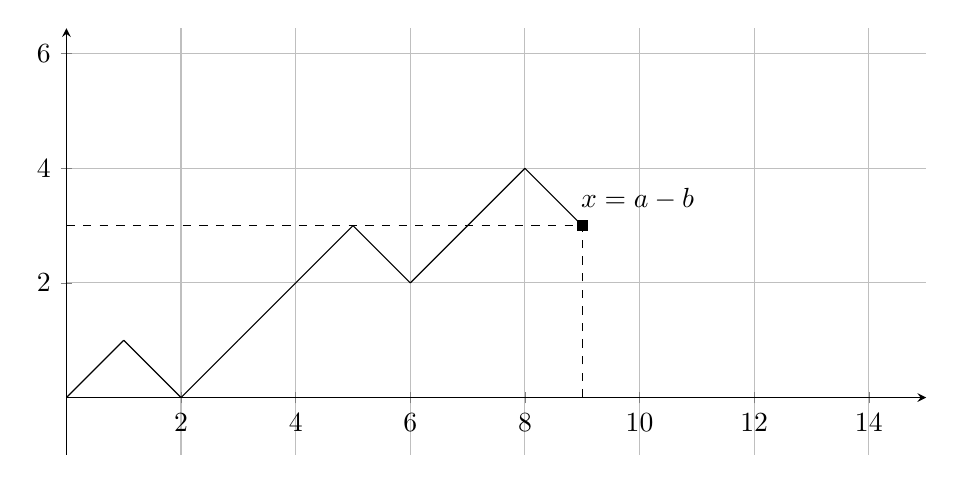
\begin{tikzpicture}
\begin{axis}[axis lines=middle, axis equal, grid=both, xmax=15, width=12.5cm, ymin=-1, height=7cm]
\addplot [color=black] coordinates{(0,0)  (1,1)};	
\addplot [color=black] coordinates{(1,1)  (2,0)};	
\addplot [color=black] coordinates{(2,0)  (3,1)};
\addplot [color=black] coordinates{(3,1)  (4,2)};
\addplot [color=black] coordinates{(4,2)  (5,3)};
\addplot [color=black] coordinates{(5,3)  (6,2)};
\addplot [color=black] coordinates{(6,2)  (7,3)};
\addplot [color=black] coordinates{(7,3)  (8,4)};
\addplot [color=black] coordinates{(8,4)  (9,3)};	
\node[label={$ \qquad\qquad x = a - b $}, fill,inner sep=2pt] at (axis cs:9,3) {};
\addplot [dashed] coordinates{(0,3) (9,3)};
\addplot [dashed] coordinates{(9,0) (9,3)};
\end{axis}
\end{tikzpicture}
\end{center}

Dove sarà la linea spezzata quando avremo estratto tutte le schede? Quando avremo fatto $ a $ passi a destra e $ b $ a sinistra, la posizione sarà $ a-b $. 

Ci chiediamo ora: qual è la probabilità che \textbf{A} sia sempre in vantaggio?

In questo caso non abbiamo tutti i cammini con probabilità uguale, perché alla fine andremo nel punto $ (n,x) $. Quanti sono i cammini che finiscono nel punto $ x $?

Abbiamo $ n $ estrazioni e dobbiamo scegliere un sottoinsieme di $ a $ elementi. Questo è quello che si chiama una combinazione. Le possibili combinazioni sono:
\begin{align*}
	& \binom{n}{a} = \frac{n!}{a!(n-a)!} \\
    = & \binom{n}{b} = \frac{n!}{b!(n-b)!} \qquad \qquad (n-b=a)
\end{align*}

Dobbiamo contare i cammini che sono sempre sopra l'asse delle x, che non toccano mai quest'asse. 

\paragraph{Principio di riflessione} com'è fatto un cammino che non tocca mai l'asse delle x? Il primo passo sarà positivo. Il principio di riflessione dice che i numero dei cammini che partono da (1,1) è uguale al numero dei cammini che partono da (1,-1) [e arrivano a x]; voglio allora contare, anziché i cammini che non passano per x, quelli che toccano l'asse:
\begin{multicols}{2}
\begin{center}
	\begin{tikzpicture}
	\begin{axis}[axis lines=middle, axis equal, xmax=15, ymin=-3, ymax=7, width=8cm, height=5cm, xtick={1}, ytick={1}]
	
	\addplot [very thick, color=black] coordinates{(0,0)  (1,1)};	
	\addplot [color=black] coordinates{(1,1)  (3,3)};	
	\addplot [color=black] coordinates{(3,3)  (5,1)};
	\addplot [color=black] coordinates{(5,1)  (10,6)};
	\addplot [color=black] coordinates{(10,6)  (12,4)};

	\node[label={$ x = a - b $}, fill,inner sep=2pt] at (axis cs:12,4) {};
	\addplot [dashed] coordinates{(0,4) (12,4)};
	\addplot [dashed] coordinates{(12,0) (12,4)};
	\addplot [color=black] coordinates{(0,1) (1,1)};
	\addplot [color=black] coordinates{(1,0) (1,1)};
	\end{axis}
	\end{tikzpicture}
\end{center}


\begin{center}
	\begin{tikzpicture}
		\begin{axis}[axis lines=middle, axis equal, xmax=15,ymin=-3, ymax=7, width=8cm, height=5cm, xtick={1}, ytick={1}]
			\addplot [very thick, color=black] coordinates{(0,0)  (1,1)};	
			
			\addplot [color=black] coordinates{(1,1)  (3,-2)};	
			\addplot [color=black] coordinates{(3,-2)  (5,0)};
			\addplot [color=black] coordinates{(5,0)  (7,-2)};
			\addplot [color=black] coordinates{(7,-2)  (12,4)};
			
			\node[label={$ x = a - b $}, fill,inner sep=2pt] at (axis cs:12,4) {};
			\addplot [dashed] coordinates{(0,4) (12,4)};
			\addplot [dashed] coordinates{(12,0) (12,4)};
			\addplot [color=black] coordinates{(0,1) (1,1)};
			\addplot [color=black] coordinates{(1,0) (1,1)};
		\end{axis}
	\end{tikzpicture}
\end{center}

\end{multicols}

L'idea è di riflettere specularmente ogni cammino che parte da (1,1) e tocca l'asse delle x.
%TODO ma l'immagine non è speculare, WTF

Questa è una corrispondenza biunivoca. 

Ci sono $ n-1 $ passi per partire da (1,1) e arrivare a $ x $. Ci sono $ a-1 $ passi a destra negli $ n-1 $ cammini da (1,1); ci sono $ a $ passi a destra partendo invece da (-1,1).

Il numero dei cammini è $ \binom{n-1}{a} $

Quanti sono i cammini che non toccano? Togliamo da tutti i cammini quelli che toccano:
$$\binom{n-1}{a-1} - \binom{n-1}{a}$$

Per calcolare la probabilità, dividiamo la quantità appena calcolata per il numero totale dei cammini:
\begin{align*}
 & \ddfrac{\binom{n-1}{a-1} - \binom{n-1}{a}}{\binom{n}{a}} = \\
 & = \ddfrac{\frac{(n-1)!}{(a-1)!(n-a)!} - \frac{(n-1)!}{a!(n-a-1)!}}{\frac{(n)!}{a!(n-a)!}} = \\
 & = \frac{1}{n}(a-b) = \\
 & = \frac{a-b}{a+b}
\end{align*}
E questa è la probabilità che il candidato A sia sempre in vantaggio su B. 

Applichiamo questo risultato alla passeggiata aleatoria simmetrica. 
Supponiamo $ S_0, S_1, ..., S_{2n} $:
$$u_{2n} = P(S_{2n} = 0 ) = \binom{2n}{n}\frac{1}{2^{2n}}$$

è la probabilità di ritrovarsi all'origine (ovvero, di fare lo stesso numero di passi sia a destra che a sinistra). $ 2^{2n} $ è il numero totale delle passeggiate possibili. 

Cosa succede quando $ n $ cresce?

\begin{tcolorbox}
	\paragraph{Formula di Stirling} 
	$$ n! = \sqrt{2\pi}\cdot n^{n+\frac{1}{2}} \cdot e^{-n} \cdot e^{\theta n} \qquad \qquad |\Theta_n| < \frac{1}{12n}$$
	
	Fornisce un'approssimazione per il fattoriale; $ \Theta_n $ è un errore che tende a 0. 
	
	Se $ n $ tende a 0, $ \Theta_n \rightarrow 0 $ e quindi $ e^{\theta_n} \rightarrow 1 $.
	
\end{tcolorbox}

Usando la formula di Stirling:
	$$ \binom{2n}{n} \frac{1}{2^{2n}} = \frac{2n!}{(n!)^2} \frac{1}{2^{2n}} = $$
	$$ = \ddfrac{\sqrt{2\pi}(2n)^{2n+\frac{1}{2}}e^{-2n} e^{\theta_{2n}}}{ (2\pi)n^{2n+1}e^{-2n}e^{2\theta_n}    }\cdot \frac{1}{2^{2n}} = $$
	$$ = \ddfrac{\sqrt{2} \cdot e^{\theta_{2n} - 2\theta_n}   } { \sqrt{2\pi}\sqrt{n}} = \frac{1}{\sqrt{\pi n}} e^{\theta_{2n} - 2\theta_n} $$

$ e^{\theta_{2n} - 2\theta_n} $ tende a 1. Il tutto tende a 0, ma abbastanza lentamente. 
\\
\\
\\
\\
\\
\\
Chiediamoci ora qual è la probabilità che la passeggiata aleatoria torni a 0 nel tempo $ 2n $ e sia sempre positiva prima di $ 2n $:
$$P(S_1 > 0, ..., S_{2n-1}>0, S_{2n} = 0)$$
Perché si verifichi occorre che $ S_{2n-1} = 1 $.
\begin{multicols}{2}
	Possiamo contare i cammini che partono da 0 e al tempo $ 2_{n-1} $ sono a 1, rimanendo sempre positivi. Lo abbiamo visto per il teorema del ballottaggio. 
	
	
	\begin{center}
		\begin{tikzpicture}
		\begin{axis}[axis lines=middle, axis equal, xmax=15,ymin=-3, ymax=7, width=6cm, height=4cm, ticks=none]
		\addplot [very thick, color=black] coordinates{(0,0)  (1,1)};	
		
		\addplot [color=black] coordinates{(1,1)  (3,3)};	
		\addplot [color=black] coordinates{(3,3)  (5,1)};
		\addplot [color=black] coordinates{(5,1)  (8,4)};
		\addplot [color=black] coordinates{(8,4)  (13,1)};
		
		\node[label={$ 2_{n-1} $}, fill,inner sep=2pt] at (axis cs:13,1) {};
		\addplot [dashed] coordinates{(0,1) (13,1)};
		\addplot [dashed] coordinates{(13,0) (13,1)};
		\end{axis}
		\end{tikzpicture}
	\end{center}
\end{multicols}

È come avere $ 2_{n-1} $ schede e $ n $ voti per A, e $ n-1 $ voti per B. Quindi, sapendo che la formula è $ \frac{a-b}{a+b} $ e che $ a $ corrisponde a $ n $ e $ b $ corrisponde a $ n-1 $, per ottenere il numero dei cammini che partono dall'origine e ritornano a 0 in $ 2n $ passi e sono sempre positivi possiamo calcolare:
$$ \frac{1}{2n-1} \cdot \binom{2n-1}{n} = \frac{(2n-1)!}{n!(n-1)!(2n-1)} = $$
$$ = \frac{(2n-2)!}{n(n-1)!^2} = \frac{1}{n} \binom{2n-2}{n-1} $$

Per calcolare la probabilità dobbiamo dividere questa quantità per il numero dei cammini totali:

$$ P(S_1 > 0, ..., S_{n-1} > 0, S_n = 0) = $$
$$ = \frac{1}{n} \binom{2n-2}{n-1} \frac{1}{2^{2n}} = \frac{1}{n}\binom{2n-2}{n-1}\frac{1}{2^{2n-2}}\frac{1}{4} = $$
$$ = \frac{1}{4n} u_{2n-2} $$

Quindi nella passeggiata aleatoria per calcolare la probabilità di un evento che si riferisce ai primi $ 2n $ passi, siccome i cammini hanno la stessa probabilità $ p $,
%TODO siamo sicuri che hanno tutti la stessa probabilità p?
 si riduce a contare quanti sono i cammini. Abbiamo visto che 
 $$ P (S_1 > 0, ..., S_{n-1} > 0, S_n = 0) = \frac{1}{n} u_{2n-2} = \frac{1}{n}\binom{2n-2}{n-1} \frac{1}{n^{n-2}}$$
 Definiamo $ L_{2n} = \frac{1}{n+1}\binom{2n}{n} $; allora possiamo riscrivere l'equazione sopra come
 $$ P(...) = L_{2n-2} \frac{1}{2^{2n-2}} $$
\\
\\
\\
\\
\\
\\
Vogliamo ora calcolare la probabilità di questo evento:
$$ P(S_1 \ge 0, S_2 \ge 0, ..., S_{2n-1} \ge 0, S_{2n} = 0) $$
Dobbiamo calcolare i cammini che rimangono maggiori o uguali a 0; la nostra passeggiata sarà di questo tipo:

\begin{center}
	\begin{tikzpicture}
	\begin{axis}[axis lines=middle, axis equal, 
	xmax=20, ymax=6, ymin=-1,
	height=6cm, width=12cm,
	ticks=none]
	
	\addplot [color=black] coordinates{(0,0)  (2,2)};	
	\addplot [color=black] coordinates{(2,2)  (3,1)};
	\addplot [color=black] coordinates{(3,1)  (4,4)};
	\addplot [color=black] coordinates{(4,4)  (8,0)};
	\addplot [color=black] coordinates{(8,0)  (9,1)};
	\addplot [color=black] coordinates{(9,1)  (10,0)};
	\addplot [color=black] coordinates{(10,0)  (12,2)};	
	\addplot [color=black] coordinates{(12,2)  (13,1)};	
	\addplot [color=black] coordinates{(13,1)  (15,3)};	
	\addplot [color=black] coordinates{(15,3)  (18,0)};	
	
	\node[label=below:{$ 2n $}, fill,inner sep=2pt] at (axis cs:18,0) {};
	\end{axis}
	\end{tikzpicture}
\end{center}


Ma possiamo ridurci al problema precedente, spostando l'origine nel punto $ (1,1) $:
\begin{center}
	\begin{tikzpicture}
	\begin{axis}[axis lines=middle, axis equal, 
	xmax=20, ymax=6, ymin=-1,
	height=6cm, width=12cm,
	xtick={1}, ytick={1}]]
	
	\addplot [color=black] coordinates{(0,0)  (2,2)};	
	\addplot [color=black] coordinates{(2,2)  (3,1)};
	\addplot [color=black] coordinates{(3,1)  (4,4)};
	\addplot [color=black] coordinates{(4,4)  (8,0)};
	\addplot [color=black] coordinates{(8,0)  (9,1)};
	\addplot [color=black] coordinates{(9,1)  (10,0)};
	\addplot [color=black] coordinates{(10,0)  (12,2)};	
	\addplot [color=black] coordinates{(12,2)  (13,1)};	
	\addplot [color=black] coordinates{(13,1)  (15,3)};	
	\addplot [color=black] coordinates{(15,3)  (18,0)};	
	
	\node[label=below:{$ 2n $}, fill,inner sep=2pt] at (axis cs:18,0) {};
	\addplot [dashed] coordinates{(0,1) (17,1)};
	\addplot [dashed] coordinates{(1,0) (1,10)};
	\addplot [color=black, very thick] coordinates{(1,0)  (1,1)};	
	\addplot [color=black, very thick] coordinates{(0,1)  (1,1)};	
	\addplot [color=black, very thick] coordinates{(17,0)  (17,1)};	
	
	\node[label={$ \qquad (2n-1, 1) $}, fill,inner sep=2pt] at (axis cs:17,1) {};
	
	
	\end{axis}
	\end{tikzpicture}
\end{center}

Il cammino spostato sarà $ \ge 0 $. Possiamo fare una corrispondenza tra i cammini compresi tra $ 0 $ e $ 2n $ di lunghezza $ 2n $, e i cammini compresi tra $ (1,1) $ e $ (2n-1, 1) $ di lunghezza $ 2n-2 $.

Il numero di cammini tra 0 e $ 2n $ sempre positivi era dato da $ \ddfrac{1}{n} \binom{\displaystyle 2n-2}{\displaystyle n-1} = L_{2n-2} $; quindi la probabilità sarà:
$$ P(S_1 \ge 0, S_{2n} = 0) = L_{2n}\frac{1}{2^{2n}} = \frac{u_{2n}}{n+1}$$
 
\paragraph{Teorema} Dato $ u_{2n} = \binom{2n}{n} \frac{1}{2^{2n}} $, allora:
\begin{enumerate}
	\item $u_{2n} = P(S_{2n} = 0)$
	\item $ u_{2n} = P(S_1 \ne 0, ..., S_{2n-1} \ne 0, S_{2n} \ne 0) $
	\item $ u_{2n} = P(S_1 \ge 0, ..., S_2n \ge 0 ) $
\end{enumerate}

Siccome abbiamo già visto 1, vogliamo dimostrare 2 e 3. 

Dimostriamo \textbf{2}; definiamo 
$$ f_{2n} = P(S_1 \ne 0, S_2 \ne 0, ..., S_{2n-1} \ne 0, S_{2n} = 0) $$

Avevamo precedentemente trovato la probabilità che il cammino fosse sempre positivo; per simmetria, è uguale alla probabilità che sia sempre negativo. Allora

$$ f_{2n} = 2P(S_1 > 0, ..., S_{2n-1} < 0, S_{2n} = 0) = 2\frac{u_{2n}-2}{n} $$

Consideriamo l'evento complementare di $S_1 \ne 0, ..., S_{2n-1} \ne 0, S_{2n} \ne 0$; è l'evento che qualche volta tra 0 e $ 2n $, $ S_i $ valga 0:

$$ P(S_1 \ne 0, ...) = 1 - f_2 - f_4 - ... - f_{2n} $$

con $ f_n $ la probabilità che $ S $ sia tornato a 0 nel tempo $ n $. 

\textbf{Osservazione:} 
$$ \underbrace{u_{2n-2} - u_{2n}}_{\displaystyle \binom{2n-2}{n-1} \frac{1}{2^{2n-2}} - \binom{2n}{n} \frac{1}{2^{2n}}} = f_{2n} $$

\begin{align*}
	\Rightarrow f_{2n} & = P(S_1 \ne 0, S_2 \ne 0, ..., S_{2n-1} \ne 0, S_{2n} = 0) = \\
	& = u_{2n-2} \Bigl(  1 - \frac{1}{4} \frac{(2n)(2n-1)}{n^2} \Bigr)  = \\
	& = u_{2n-2} \Bigl(\frac{2n - 2n + 1}{2n} \Bigr) = \\
	& = \frac{u_{2n-2}}{2n} = f_{2n} 
\end{align*}

$$ \Rightarrow 1 - f_2 - f_4 - ... - f_{2n} = 1 - (u_0 - u_2) - (u_2) - u_4 - ... - (u_{2n-2} - u_{2n}) = u_{2n}. \qed \text{ QED }$$ 

$ u_0 $ per definizione è 1; $ u_2 $ si cancella con $ u_2 $ (gli $ u_i $ si cancellano due alla volta).

Interpretazione: sappiamo, per Stirling, che possiamo approssimare $ u_{2n} \approx \frac{1}{\sqrt{\pi n}} $. Se prendiamo $ n $ grande. la probabilità che non si torni mai a 0 tende a 0. Ad esempio, se prendiamo 2 giocatori A, B che tirano una moneta, e se esce testa A vince 1 euro (e B perde), mentre se esce croce A perde un euro (e B vince), la probabilità che il gioco non termini mai e che i giocatori vanno avanti all'infinito tende a 0. 
\\
\\
Dimostriamo \textbf{3}; vogliamo dimostrare che $ u_{2n} = P(S_1 \ge 0, ..., S_2n \ge 0 ) $, che rappresenta l'evento che il primo giocatore (sempre nell'esempio dei due giocatori che tirano una moneta) sia sempre in vantaggio o in parità. 

Definiamo 
$$ f_{2n} = P(S_1 \ge 0, ..., S_{2n-2} \ge 0, S_{2n-1} < 0) $$
in base al conteggio fatto precedentemente sul numero dei cammini $ \ge 0 $ fino a $ 2n-2 $, questa quantità è pari a:
$$  f_{2n} = \frac{1}{2^{2n} u_{2n-2} \frac{1}{2n}} $$

Consideriamo l'evento complementare di $ f_{2n} $, cioè che ci sia stato un punto negativo. I punti negativi possono essere solo nei punti dispari:

\begin{align*}
 P(S_1 \ge 0, ..., S_{2n-2} \ge 0, S_{2n-1} < 0) & = \\
 & = 1 - f_2 - ... - f_{2n} = 1 - (u_0 - u_2) - ... - (u_{2n-2 - u_{2n}}) \\
 & = u_{2n} \qed \text{ QED }
\end{align*}

\paragraph{Equazione del rinnovamento} c'è una relazione che collega $ u_{2n} $ e $ f_{2n} $, si chiama \textit{equazione del rinnovamento} (renewal equation):

$$ u_{2n} = \sum_{r = 1}^{n} f_{2r} u_{2n-2r} $$

\begin{multicols}{2}
	Se abbiamo un cammino che va da 0 a $ 2n $, si può decomporre in due parti: quella che va da 0 a 0 per la prima volta, e da lì a $ 2n $. Chiamiamo il primo tempo $ 2r $. 
	
	
	\begin{tikzpicture}
	\begin{axis}[axis lines=middle, axis equal, 
	xmax=20, ymax=6, ymin=-2,
	height=5cm, width=9cm, ticks=none]
	
	\addplot [color=black] coordinates{(0,0)  (2,2)};	
	\addplot [color=black] coordinates{(2,2)  (3,1)};
	\addplot [color=black] coordinates{(3,1)  (4,4)};
	\addplot [color=black] coordinates{(4,4)  (9,-1)};
	\addplot [color=black] coordinates{(9,-1)  (12,2)};
	\addplot [color=black] coordinates{(12,2)  (13,1)};	
	\addplot [color=black] coordinates{(13,1)  (15,3)};	
	\addplot [color=black] coordinates{(15,3)  (18,0)};	
	
	\node[label=below:{$ 2n $}, fill,inner sep=2pt] at (axis cs:18,0) {};
	
	\node[label=below:{$ 2r $}, fill,inner sep=2pt] at (axis cs:8,0) {};
	
	
	\end{axis}
	\end{tikzpicture}
\end{multicols}

Il numero totale dei cammini è $ \binom{2n}{n} $

$$ u_{2n} 2^{2n} \binom{2n}{n} = \sum_{r=1}^{n} f_{2r}2^{2r} u_{2n-2r}2^{2n-2r} $$

se dividiamo a sinistra e a destra per $ 2^{2n} $ otteniamo l'equazione di rinnovamento.
\\
\\
\\
\\
\\
\\
Abbiamo due giocatori, A e B, che tirano una moneta: se esce testa, A vince un euro (e B perde), viceversa A perde un euro (e B vince); ci chiediamo qual è la percentuale di tempo in cui uno dei due è in vantaggio. Si potrebbe pensare che sia A che B rimangano in vantaggio per circa il 50\% del tempo. In realtà, quando $ N $ (numero di lanci) è grande, è più probabile che un solo giocatore rimanga in vantaggio tutto il tempo. 

\begin{multicols}{2}
		\begin{tikzpicture}
			\begin{axis}[axis lines=middle, axis equal, 
			xmax=20, ymax=6, ymin=-2,
			height=5cm, width=7cm, ticks=none]
			
				\addplot [color=black] coordinates{(0,0)  (2,2)};	
				\addplot [color=black] coordinates{(2,2)  (6,-2)};
				\addplot [color=black] coordinates{(6,-2)  (11,3)};
				\addplot [color=black] coordinates{(11,3)  (13,1)};
				\addplot [color=black] coordinates{(13,1)  (16,4)};
	
								
				\node[label=below:{$ 2n $}, fill,inner sep=2pt] at (axis cs:16,0) {};
				

			\end{axis}
		\end{tikzpicture}
	
	
	Come definiamo il tempo in cui un giocatore è in vantaggio sull'altro? Se rappresentiamo nel grafico la passeggiata aleatoria, essa sarà una linea spezzata; ma invece di considerare i tempi discreti, immaginiamo che la linea sia il grafico di una funzione.
\end{multicols}

Consideriamo la lunghezza dell'intervallo in cui la funzione è positiva. Definiamo 

\formule{  P_{2k, 2n} = }{ probabilità che il primo giocatore sia in vantaggio per un tempo $ 2k $}

È stato dimostrato (Fenner) che $ P_{2k, 2n} = u_{2k}u_{2n-2k} $. Si dimostra per induzione su $ n $:

\textbf{Caso base: } $ p_{0,2n} $ = probabilità che il primo giocatore sia sempre in vantaggio o pari ($ S \ge 0 $)

$ p_{0, 2n } = P(S_1 \ge 0, ..., S_{2n} \ge 0) = u_{2n} \qed$

\textbf{Caso induttivo: } supponiamo che l'uguaglianza valga per $ n-1 $; dimostriamo che vale per $ n $. 

Sia $ 1 \le k \le n-1 $. Ci sarà un intervallo in cui il grafico è sopra e uno in cui il grafico della passeggiata aleatoria è sotto l'asse x; ad un certo punto quindi passerà per l'asse x (y=0). Quindi, il primo intervallo può essere positivo o negativo; il secondo sarà l'opposto. 

$$ p_{2k, 2n} = \underbrace{\sum_{r=1}^{k}\frac{1}{2} f_{2r} p_{2k-2r, 2n-2r}}_{\substack{\text{probabilità di tornare a 0 per} \\ \text{la prima volta al tempo 2r; il} \\ \text{cammino può essere positivo} \\ \text{o negativo, per questo} \\ \text{moltiplichiamo per } \frac{1}{2}}}       + \sum_{r=1}^{n-k} \frac{1}{2}f_{2r}p_{2k, 2n-2r} =  $$ 
%TODO ambiguità: da una parte si dice che la prima sommatoria rappresenta la probabilità di tornare a 0 e il cammino era positivo, mentre la seconda sarebbe la stessa p con il cammino negativo; da un'altra parte si dice che il cammino può essere positivo o negativo, non lo sappiamo, per questo moltiplichiamo per 1/2
$$ = \frac{1}{2} \sum_{r=1}^{k} f_{2r}u_{2k-2r}u_{2n-2k} + \frac{1}{2}\sum_{r=1}^{n-k}f_{2r}u_{2k}u(2r-2k) - 2r$$
Applichiamo la formula del rinnovamento:
\begin{align*}
	& = \frac{1}{2}u_{2n-2} + \sum_{r=1}^{k}f_{2n}u_{2k-2r} + \frac{1}{2}u_{2k}\sum_{r=1}^{n-k}f_{2r} u2(n-k) - 2r \\
	%TODO non capisco se u2(n-k) - 2r in realtà vada come pedice, cioè u_{2(n-k) - 2r}
	& = \frac{1}{2} u_{2n-2k}u_{2k} + \frac{1}{2}u_{2k}u_{2n-2k} \\
	& = u_{2k}u_{2n-2k} \qed 
\end{align*}

\paragraph{Esempio} consideriamo i soliti 2 giocatori che scommettono su testa o croce; supponiamo 20 lanci di moneta. 

$ p_{2k,20} $ è la probabilità che il primo giocatore sia in vantaggio esattamente un tempo $ 2k $.

$ P_{2k,20} $ è la probabilità che il primo giocatore sia in vantaggio almeno un tempo $ 2k $.

\begin{center}
	\begin{tabular}{ c|c|c|c|c|c|c }	

		 & $ k= 0, k = 10 $ & $ k=1, k=9 $ & $ k=2, k=8 $ & $ k=3, k=7 $ & $ k=4, k=6 $ & $ k=5 $ \\
		\hline
		
		p & 0,1702 & 0,0927 & 0.0736 & 0.0655 & 0.0617 & 0.064 \\
		P & 0.3504 & 0.5379 & 0.6851 & 0.8160 & 0.9394 & 1 
		
	\end{tabular}
\end{center}

Possiamo ricavare una legge generale, facendo tendere $ n $ all'infinito e osservando come si comporta la quantità $ p_{2k, 2n} $.

Anziché $ k $ consideriamo $ \frac{k}{n} = x $, cioè consideriamo la percentuale del tempo in cui il primo giocatore è in vantaggio. $ x $ assume valori discreti:

\formule{x = }{0, $\frac{1}{n}, ..., 1$}

Un modo per rappresentare la distribuzione di probabilità è attraverso l'istogramma:

\begin{multicols}{2}
	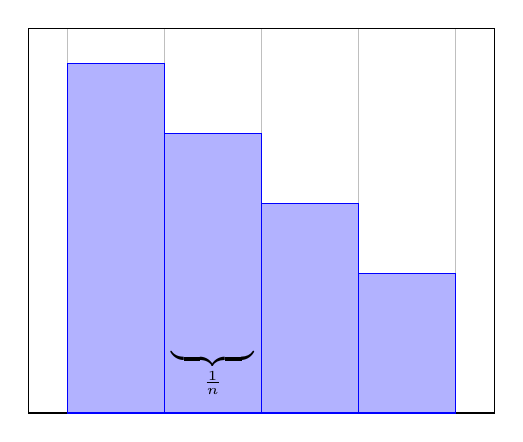
\begin{tikzpicture}
		\begin{axis}[ybar interval, ymax=55,ymin=0, ticks=none, width=7.5cm]
			\addplot coordinates { (10, 50) (15, 40) (20, 30) (25, 20) (30,10) };
			
			\node[label={$ \underbrace{\qquad \quad}_{\frac{1}{n}} $},inner sep=2pt] at (axis cs:17.5,0) {};
		\end{axis}
	\end{tikzpicture}
	
	
	L'area del rettangolo è uguale alla probabilità che assuma un certo valore. 
	Abbiamo visto per Stirling che $ u_{2n} \approx \frac{1}{\sqrt{\pi n}} $. 
	Supponiamo $ n $ grande e $ 0 \le k \le n $; allora possiamo scrivere:
		$$ u_{2k} u_{2n-2k} \approx \frac{1}{2\pi}\frac{1}{\sqrt{k(n-k)}} $$
	
\end{multicols}

Riscriviamo la funzione in termini di $ x $ e chiamiamola $ g $:

$$ g(x) \approx \frac{1}{n2\pi} \frac{1}{\sqrt{x(1-x)}} $$

Da questa formula si vede che l'istogramma è vicino alla funzione $ \frac{1}{2\pi\sqrt{x(1-x)}} $:

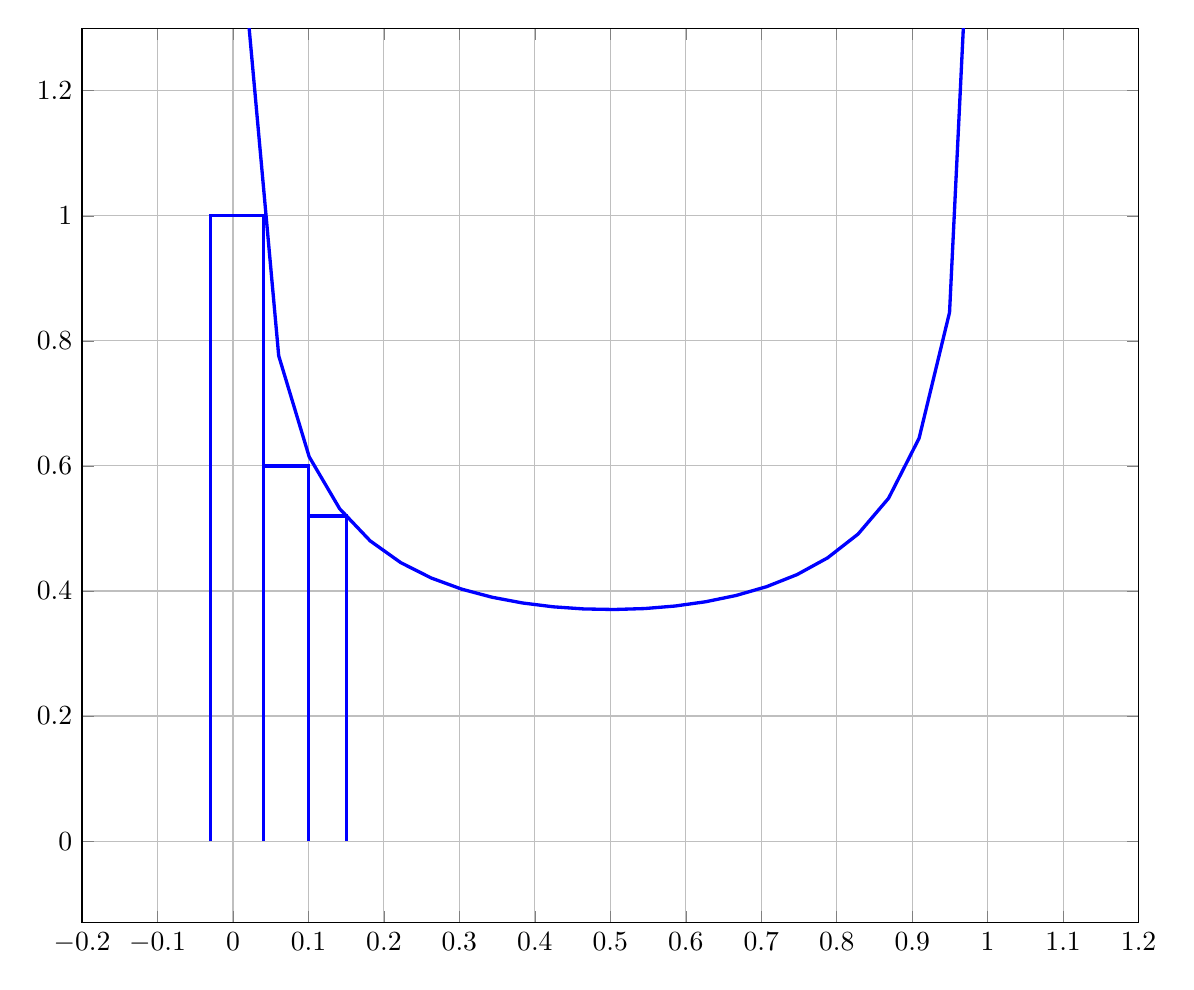
\begin{tikzpicture}
	\begin{axis}[grid=major, width=15cm, xmin=-0.2, xmax=1.2, ymax=1.3]
		%\addplot coordinates { (0, 5) (5, 35) (10, 50) (15, 30) (20, 15) (25, 0) };
		
		\addplot[color=blue, very thick, domain=-2:2, samples=100]	
		{1/(2 * 2.7 *sqrt(x*(1-x)) )};
		
		\addplot [color=blue, very thick] coordinates { (-0.03, 0) (-0.03, 1) (0.04, 1) (0.04, 0) };
		\addplot [color=blue, very thick] coordinates { (0.04,0) (0.04, 0.6) (0.1, 0.6) (0.1, 0)};
		\addplot [color=blue, very thick] coordinates { (0.1, 0) (0.1, 0.52) (0.15, 0.52) (0.15, 0) };

	\end{axis}
\end{tikzpicture}

Dobbiamo fare la somma di tutti i rettangoli sotto la funzione $ \frac{1}{2\pi\sqrt{x(1-x)}} $. Questa è la somma di Riemann, un'approssimazione dell'integrale:
$$ \approx \sum_{\frac{1}{2} < x < z} \frac{1}{n2\pi} \frac{1}{\sqrt{x(1-x)}} $$
$$ \to_{n \to \infty} \int_{\frac{1}{2}}^{z} \frac{1}{\pi \sqrt{x(1-x)}} dx$$ 

Con riferimento al grafico precedente, si vede che quando $ x $ tende a 0 oppure a 1, la probabilità tende all'infinito, mentre a $ \frac{1}{2} $ è nel punto più basso. 

Questa è detta \textbf{prima legge dell'arcoseno} perché la primitiva dell'integrale è uguale a:
$$ \int \frac{1}{\pi \sqrt{x(1-x)}} dx = 2\pi^{-1} \arcsin {\sqrt{x}} + c$$
%TODO controlla sia \pi^{-1}

La prima legge dell'arcoseno è un'approssimazione della probabilità che uno dei due giocatori sia in vantaggio una certa percentuale di volte, per un $ n $ grande. 

Questo vale per la passeggiata aleatoria asimmetrica libera. 
\\
\\
\\
\\
\\
\\
Vediamo un caso simile: consideriamo la probabilità che il primo giocatore sia in vantaggio per un tempo $ 2k $ e che a $ 2n $ la passeggiata sia 0, ovvero i due giocatori siano in pareggio; definiamo

\formule {(   \frac{1}{2^{2n}}) (L_{2k,2n}) = } { probabilità che il primo giocatore  sia in vantaggio per un tempo $ 2k $ e che $ s_{2n} = 0 $}

$ L_{2k, 2n} $ è il numero dei cammini; dividendolo per il numero totale dei cammini $ 2^{2n} $ dà la probabilità. 

Allora $ L_{2k, 2n} = L_{2n} $, e avevamo definito $ L_{2n} = \ddfrac{1}{n+1}	\binom{\displaystyle 2n}{\displaystyle n} $.

È possibile dimostrare che il numero dei cammini non dipende da $ k $, ma è lo stesso per tutti i valori di $ k $; qualsiasi percentuale ha la stessa probabilità.

\paragraph{Dimostrazione} per induzione su $ n $:
\begin{multicols}{2}
	\begin{tikzpicture}
		\begin{axis} [axis equal, axis lines=middle , ticks = none, ymin = 0, ymax = 7, xmin = -3, xmax = 20, width=7.5cm, height=6cm]
			\addplot [color = black] coordinates { (0,0) (2,2) (4,0) (8,4) (9,3) 
							(10,4) (14,0) (16,2) (18, 0)};
			\node [ label=below left:0 ] at (axis cs:0,0) {};
			\node [ label=below: $ 2n $ ] at (axis cs:18,0) {};
		\end{axis}
	\end{tikzpicture}
	
	
	Supponiamo sia vero per $ n-1 $; vogliamo vedere che la proprietà vale anche per $ n $
	%TODO supponiamo sia vero che cosa?
	Supponiamo $ k = n $. Dobbiamo contare i cammini che tornano a 0 e sono sempre $ \ge $ 0; ma lo abbiamo già visto: i cammini sono $ L_{2n, 2n} = \ddfrac{1}{n+1}\binom{\displaystyle n}{\displaystyle n} $.


	Anche il caso $ k = 0 $ lo abbiamo già visto. 
	
\end{multicols}

Supponiamo $ 1 \le k \le n-1 $. Questo cammino deve passare per forza per 0, perché una parte del tempo è in vantaggio il primo giocatore, l'altra il secondo. Sia $ 2r $ il primo istante in cui la passeggiata passa per lo 0. Fino al tempo $ 2r $, il cammino può essere positivo o negativo. 

$$ L_{2k,2n} = \sum_{r=1}^{k} L_{2r-2} L_{2n-2r} + \sum_{r=1}^{n-k} L_{2r-2} L_{2n-2r}$$

%TODO controlla equazione

Modifichiamo la variabile $ r $ al secondo membro, con $ \rho = n -r + 1 $. Quindi 
\begin{align*}
	& \text{per } r = n - k, & \qquad \rho = k + 1 \\
	& \text{per } r = 1, & \qquad \rho = n
\end{align*}

$$ = \sum_{r=1}^{k}L_{2n-2}L_{2n-2r} + \sum_{\rho = k+1}^{n} L_{2\rho - 2} L_{2n - 2\rho}$$

$$ = \sum_{r=1}^{n} L_{2r-2}L{2n-2r} \qed$$

Abbiamo dimostrato che $ L_{2k,2r} $ non dipende da $ k $, ma è uguale per tutti i valori. Ma quanto vale effettivamente?

$ L_{0, 2n} = L_{2n,2n} = L_{2n} $

$ L_{k,2n} $ per $ k = 1, n = 1 $ sono uguali

Supponiamo che: 
$$ \sum_{k=0}^{n} L_{2k,2n} = \binom{2n}{n} $$
facendo variare $ k $ da 0 a $ n $ otteniamo tutti i cammini di lunghezza $ 2n $

Supponiamo $ 1 \le k \le n-1 $:

\begin{align*}
	L_{2k, 2n} & = \frac{\binom{2n}{n} - 2L_{2n}}{n-1} = \\
	& = \frac{\binom{2n}{n} - \frac{2\binom{2n}{n}}{n+1}}{n-1} = \binom{2n}{n} \frac{1 - frac{2}{n+1}}{n-1} \\
	& = \binom{2n}{n}\frac{\frac{n+1-2}{n+1}}{n-1} = \frac{\frac{2n}{n}}{n+1} \\
	& = L_{2n}
\end{align*}

\section{Problema della rovina del giocatore (gambler's ruin)}
Consideriamo un altro problema, la rovina del giocatore. È sempre basato su una passeggiata aleatoria. Consideriamo 2 giocatori A e B che tirano una moneta; se esce testa, A vince 1 euro; se esce croce, perde 1 euro (e lo vince B). Ci chiediamo quale sia il capitale del primo giocatore dopo un certo numero di giocate. 

Supponiamo che al tempo 0 il capitale iniziale di A sia $ x $, mentre il capitale di B ammonti a $ N - x $. Il capitale totale (capitale di A + capitale di B) ammonta quindi a $ N $. Se il capitale di uno dei due giocatori arriva a 0, il gioco si ferma (e si ha la rovina del giocatore). 

Considereremo anche il caso della \textbf{moneta non simmetrica}, dove cioè la probabilità $ p $ che esca testa è $ 0 < p < 1 $. I lanci sono indipendenti tra loro.

Ci chiediamo qual è la probabilità che dopo un certo numero di giocate A oppure B sia rovinato. Non supponiamo ci sia un numero finito di lanci, il gioco potrebbe teoricamente continuare all'infinito. 

Definiamo le seguenti quantità:
\formule{E_i = }{i-esimo lancio è testa (evento)}

$$ P(E^*_1, ..., E^*_n) = p^k(1-p)^{n-k} $$


\begin{equation}
	E^*_i=
	\begin{cases}
		E_i, & \text{se l'evento è verificato}  \\
		\tilde{E}_i, & \text{altrimenti}
	\end{cases}
\end{equation}

Con $ k $ numero degli eventi $ E_i $ e $ n-k $ numero degli eventi $ \tilde{E}_i $.

Questo schema di Bernoulli formalizza il fatto che i lanci siano indipendenti. 

Definiamo

\formule{u_x = }{probabilità di rovina del giocatore A con capitale iniziale $ x $, contro B con capitale iniziale $ N-x $}

\paragraph{Caso simmetrico } $ p = \ddfrac{1}{2} $

Supponiamo $ 0 < x < N $. Osserviamo in generale che $ u_0 = 1 $ e $ u_N = 0 $.

Possiamo scrivere $ u_x $ come la probabilità di rovina del giocatore sapendo che il primo lancio ha dato testa sommata alla probabilità di rovina del giocatore sapendo che il primo lancio ha dato croce:
\begin{align*}
	u_x & = p\cdot u_{x+1} + (1-p)\cdot u_{x-1} \\
	& = \frac{1}{2}u_{x-1} + \frac{1}{2}u_{x+1} = \cancel{\frac{1}{2}}(u_{x+1} - u_{x}) = \cancel{\frac{1}{2}}(u_x - u_{x-1}) \\
	& u_{x+1} - u_x = c \text{ \qquad (la differenza tra due valori successivi è sempre uguale, la chiamiamo } c) \\ \\
	0 & = u_n = u_0 + \sum_{x=0}^{N-1}(u_{x+1} + u_x)\\
	0 & = u_n = 1 + N_c \Rightarrow c = -\frac{1}{N} \\
	u_x & = u_0 + \sum_{y=0}^{x-1} (u_{y+1} - u_y) = 1 - \frac{x}{N}
\end{align*}

Quindi se $ x \to N $, la probabilità che A si rovini tende a 0. Cosa succede se $ N $ tende all'infinito? A parte da $ x $, e B da $ N - x $. La probabilità di rovina in questo caso tende a 1. 

La probabilità che il gioco continui all'infinito è 0.

\paragraph{Caso non simmetrico} $ 0 < p < 1 $
Nel caso $ p = \ddfrac{1}{2} $ le differenze erano uguali (al valore $ c $). Nel caso non simmetrico questo non vale. Occorre introdurre la \textbf{somma geometrica}:

supponiamo $ \alpha \ne 1 $:
\begin{align*}
	S & = \sum_{k=0}^n \alpha^k = \ddfrac{\alpha^{n+1} - 1}{\alpha - 1} \\
	\alpha S & = S - 1 + \alpha^{N+1} - 1 \\
	(\alpha - 1)S & = \alpha^{N+1} - 1 \\
	S & = \ddfrac{\alpha^{N+1} - 1}{\alpha - 1} \qquad \qquad \begin{cases}
		\alpha < 1, & \text{la serie è convergente} \\
		\alpha > 1, & \text{la serie va avanti all'infinito}
	\end{cases}
\end{align*}

Tornando a noi, abbiamo detto che nel caso simmetrico $ 0 < p < 1 $; se $ p > \ddfrac{1}{2} $ A è favorito, altrimenti è favorito B. Sia ancora $ u_x $ la probabilità di rovina di A, e scriviamola ancora come la somma delle probabilità della rovina del giocatore se il primo lancio è testa oppure è croce:
$$ 0 < x < N \qquad \qquad \qquad u_x = p\cdot u_{x+1} + q\cdot u_{x-1} $$
Con $ q = 1-p $. 

\begin{align*}
	(p+q)u_x & = pu_x + q_ux = pu_{x+1} + qu_{x-1} \\
	q(u_x - u_{x-1})  & = p(u_{x+1} - u_x) \\
	u_{x+1} - u_x & = \frac{q}{p}(u_x - u_{x-1}) \\
	u_{k+1} - u_k & = (\frac{q}{p})^k(u_1 - u_0) \qquad \qquad u_0 = 1 \text{ (rovina all'istante iniziale), } u_N = 0 \\
	u_k & = u_0 + \sum_{j=0}^{k-1}(u_{j+1} - u_j) \\
	& = 1 + \sum_{j=0}^{k-1}(\frac{q}{p})^j(u_1 - u_0) \\
	& = 1 + (u_1 - u_0) \sum_{j=0}^{k-1} (\frac{q}{p})^j \\
	\text{possiamo} & \text{ applicare la formula della somma geometrica } (p\ne \frac{1}{2} \Rightarrow \frac{q}{p} \ne 1): \\	 
	 & = 1 + (u_1 - u_0)\ddfrac{\left(\ddfrac{q}{p}\right)^k - 1}{\ddfrac{q}{p} - 1}
\end{align*}

Applichiamo la formula per $ k = N $, sapendo che $ u_N = 0 $:

$$ 0 = 1 + (u_1 - u_0) \ddfrac{\left(\ddfrac{q}{p}\right)^N - 1}{\ddfrac{q}{p} - 1} $$

$$ u_1 - u_0 = - \ddfrac{\ddfrac{q}{p} - 1}{\left(\ddfrac{q}{p}\right)^N - 1} $$

Possiamo calcolare $ u_k $ in generale:
$$ u_k = 1 - \ddfrac{\left(\ddfrac{q}{p}\right)^k - 1}{\left(\ddfrac{q}{p}\right)^N - 1} $$

che è la probabilità di rovina di A che parte con capitale iniziale pari a $ k $. 

Consideriamo ora $ v_k $ la probabilità di rovina di B; in questo caso B vince con probabilità $ q $.

$$ v_k = 1 - \ddfrac{\left(\ddfrac{p}{q}\right)^{N-k} - 1}{\left(\ddfrac{p}{q}\right)^N - 1} $$

$ v_k + u_k = 1 $. La probabilità che il gioco continui all'infinito è 0 (uno dei due giocatori va in rovina prima o poi). Cosa succede se $ N \to \infty $ (con $ p \ne \frac{1}{2} $)? Supponiamo $ p > \frac{1}{2} $. 

$$ \frac{q}{p} < 1 \qquad \qquad u_k \stackrel{N \to \infty}{\longrightarrow} \left(\frac{q}{p}\right)^k \qquad (\text{perché} \left(\frac{q}{p}\right)^N \to 0, \text{ perché } \frac{q}{p} < 1) $$

Quindi se A è favorito, la sua probabilità di rovina è minore di 1, e più è grande $ k $ e più si abbassa.

Se $ p < \ddfrac{1}{2} $: $ \ddfrac{q}{p} > 1 $ e $ u_k \stackrel{N \to \infty}{\longrightarrow} 1 $.

\section{Processi di diramazione di Galton-Watson (branching processes)}
Sono esempi particolari delle catene di Markov, un modello più generale. Servono per studiare l'evoluzione di una popolazione. È un modello molto semplificato; partiamo supponendo di avere un solo individuo che avrà un certo numero di figli. 

Supponiamo che ogni individuo abbia le stesse probabilità di avere figli, indipendentemente dagli altri individui, e gli intervalli (numero di figli) siano regolari. Consideriamo una successione di variabili aleatorie, e vogliamo vedere quanti figli ci sono nelle varie generazioni.

Definiamo:
\formule{x_i = }{numero di figli della generazione i-esima}
\formule{p_k = }{probabilità di avere $ k $ figli per ogni individuo; $ \sum_{k=0}^\infty p_k = 1 $ (sono eventi incompatibili, è una partizione).}

Supponiamo che l'attesa del numero di figli sia finita; la indichiamo con $ \mu $:
$$ \mu = \sum_{k=0}^{\infty} k \cdot p_k < +\infty $$

Quindi abbiamo supposto $ x_0 = 1 $. Qual è l'attesa della k-esima generazione?

\begin{tcolorbox}
	\paragraph{Formula delle probabilità totali} date due variabili aleatorie $ A $ e $ B $ , possiamo chiederci quanto vale l'\textit{attesa condizionata}, ovvero la probabilità che si verifichi $ A $ sapendo che $ B $ assume un certo valore $ x $:
		$$ P(A | B = x) $$
	Possiamo conoscere l'attesa non condizionata con la formula delle probabilità totali:
		$$ P(X) = \sum_{x=0}^{\infty} P(A|B=x)P(B=x) $$
\end{tcolorbox}

Siano $ x $ e $ y $ due variabili aleatorie a valori interi. Ci possiamo chiedere l'attesa di $ x $ quando $ y $ assume certi valori: $ P(x | y = j) $; usando la formula delle probabilità totali: 
$$ P(x) = \sum_{j=0}^{\infty} P(x | y = j)P(y=j) $$

Vogliamo calcolare l'attesa di $ k $:
\begin{align*}
	P(x_k) & = \sum_{j=0}^{\infty} P(x_k | x_1 = j)P(x_1 = j) \\
	& = \sum_{j=0}^{\infty} jp_jP(x_{k-1}) \\
	& = \mu P(x_{k-1})
\end{align*}

Possiamo dividere la j-esima generazione nei figli dell'individuo 0; %TODO ah si? ha senso?
possiamo suddividerla in $ j $ sottoinsiemi e calcolare l'attesa dei sottoinsiemi:
$$ P(x_k) = \mu P(x_{k-1}); \qquad \qquad P(x_0) = 1 \text{ (per ipotesi)}; \qquad \qquad P(x_k)=\mu^k$$

Se $\mu < 1$, avremo l'estinzione:
\formule{E_k(x_k=0)}{evento che al tempo $ k $, $ x_k=0 $}
\formule{E_k \subset E_{k+1}}{$ A $ è contenuto in $ B $ se quando si verifica il primo, allora si verifica anche il secondo}
\formule{E = \bigvee_{k=1}^\infty E_k}{si verifica almeno uno degli eventi}

(Nota: $\bigvee$ indica la somma logica, si può usare anche $\bigcup$).
\\
\\
\\
%TODO sugli appunti c'è un titolo: LIQUIDITÀ (?) NUMERABILE
Se abbiamo una successione di eventi crescenti ($ E_k \subset E_{k+1} $), allora
$$ P(E) = \underset{k}{sup} \: P(E_k)$$
Vogliamo mostrare che se $\mu < 1$, allora $ P(E) = 1 $:
\begin{align*}
	P(E_k) & = 1 - P(\tilde{E}_k) \\
	& = 1 - \sum_{j=1}^{\infty}P(x_k = j) \ge 1 - \sum_{j=1}^{\infty}jP(x_k=j) \\
	& = 1 - P(x_k) \\
	& = 1-\mu^k \to 1 \qquad \qquad \text{perché abbiamo supposto } \mu < 1 \Rightarrow \mu^k \stackrel{k \to \infty}{\longrightarrow} 0 \\ \\
	& P(E) = 1
\end{align*}(

Se invece $\mu = 1$, l'attesa di $ x_k(P(x_k)) $ rimane 1.

Vediamo infine il caso generale: non facciamo ipotesi su $\mu$, ma può assumere qualsiasi valore.

Sia $ \Pi^k = P(x_k = 0) $.

Possiamo usare la formula delle probabilità condizionate:
$$ \Pi^k = P(x_k = 0) = \sum_{j=0}^{\infty} P(x_k = 0 | x_1 = j) P(x_1 = j) $$
$$ = \sum_{j=0}^{\infty} p_j\Pi^{(k-1)j} $$  %TODO forse questo p_j è in realtà P_j

%TODO controlla anche che i \Pi non siano in realtà \pi e viceversa (nelle equazioni più in basso)
Affinché nella k-esima generazione non ci siano più individui, in tutti i rami ci deve essere l'estinzione. 

Definiamo una funzione $ f $:
\begin{align*}
	f(s) & = \sum_{j=0}^{\infty} p_j s^j \\
	\pi^k & = f(\pi^{k-1}) \\
	\pi^k \ge \pi^{k-1} \qquad \qquad \pi^k \le 1
\end{align*}

Abbiamo una successione non decrescente:
$$ \pi = P(E) = \underset{k}{sup} \: \pi^k $$

Ipotizziamo che $ p_0 + p_1 < 1 $ e $ p_0 > 0 $.

Se $ p_0 = 0$, vorrebbe dire che la p che un individuo non abbia figli sia 0. Allora ls $ P(E) $ (probabilità di estinzione) sarebbe 0. 

Supponiamo ora $ p_0 + p_1 = 1 $ e $ p_0 > 0 $, ovvero ogni individuo non ha figli, oppure ha un solo figlio: allora $ P(E) = 1 $ (si ha estinzione).

Studiamo com'è fatta $ f(s) $:

$$
\begin{array}{ccc}
	f(1) = 1 & \qquad f'(s) = \sum_{j=1}^{\infty} j \cdot p^j \cdot s^{j-1} & f''(s) > 0 \\
	f(0) = p_0 > 0 & \quad f'(1) = \sum_{j=1}^{\infty} j \cdot p^j = \mu & \quad f''(s) = \sum_{j=2}^{\infty} p_j \cdot j \cdot (j-1) s^{j-2} > 0, \quad 0 < s < 1
\end{array}
$$

La derivata seconda è positiva, quindi la funzione è strettamente convessa.

\begin{tikzpicture}
	\begin{axis}[grid=major, axis lines = middle, width=15cm, xmin=-0.2, xmax=1.2, ymax=1.1, ymin=-0.1, xtick={1}, ytick={1}]
	%xtick={0.417, 0.805, 1}, ytick={0.417, 0.65, 1}
		\addplot[color=blue, very thick, domain=0:1, samples=300]	
		{0.4 + 0.6*x*x*x*x}; %Se stai leggendo i sorgenti, questa è una funzione a caso che mi sono inventato
		
		\addplot [color=blue] coordinates { (0, 0.4) (1, 1)};
		\addplot [color=blue, dashed] coordinates { (0,0) (1,1)};
		
		\addplot [color=orange] coordinates { (0.417, 0) (0.417, 0.417) (0.417, 0.65) 
		(0.805, 0.65) };
	
		\addplot [color=orange] coordinates { (0, 0.417) (0.417, 0.417) };
		
		\node [ circle, fill, draw=black, scale=0.5, label=below left:$ p_0 $ ] at (axis cs:0,0.4) {};
		\node [ circle, fill, draw=black, scale=0.5, label=above right:$f(1)$ ] at (axis cs:1,1) {};
		\node [ label=below:$ \pi^{(1)} $] at (axis cs:0.417, 0) {};
		\node [ label=above:$ \pi^* $] at (axis cs:0.805, 0.65) {};
		
	
	\end{axis}
\end{tikzpicture}

Qual è la probabilità di estinzione? $ \pi = f(\pi) $; la probabilità di estinzione è una soluzione di una delle funzioni sottostanti:

$ \pi^{(1)} = p_0 $ (prima generazione)

$ \pi^{(2)} = f(\pi^{(1)}) $

$ \pi^{(3)} = f(\pi^{(2)}) $

$ \pi^{(k+1)} = f(\pi^{(k)}) $

Siccome $ f $ è crescente, se applichiamo da entrambe le parti:

$ p_0 < \pi^* $

$ \pi^{(1)} < \pi^* $

...

$ \pi^t < \pi^* $

Questa successione rimane sempre più piccola di $\pi^*$, quindi il limite tenderà a $ \pi^* $, che è minore di 1.

Quindi se $ \mu > 1$, c'è una probabilità positiva che non ci sia estinzione. 
%TODO qualcosa non torna: \mu è la probabilità di estinzione, secondo me la frase sopra è "se ??? > 1, allora \mu < 1 (cioè c'è una probabilità positiva che non si estinugano - ovvero 1 - \mu)

%TODO manca grafico con caso \mu >= 1

\paragraph{Esempi} vediamo alcuni esempi:
\begin{itemize}
	\item $ p_0 = \frac{1}{2}, p_1 = \frac{1}{4}, p_2 = 0, p_3 = \frac{1}{4} $
	
	$ \mu = 0 \cdot \frac{1}{2} + 1 \cdot \frac{1}{4} + 2 \cdot 0  + 3 \cdot \frac{1}{4} = 1 \Rightarrow \pi = 1$
	\item $ p_0 = \frac{1}{3}, p_1 = \frac{1}{3}, p_2 = 0, p_3 = \frac{1}{3} $
	
	$ \mu = 0 \cdot \frac{1}{3} + 1 \cdot \frac{1}{3} + 2 \cdot 0  + 3 \cdot \frac{1}{3} = \frac{4}{3} > 1$
	
	Per calcolare $\pi$ dobbiamo risolvere:
	\begin{align*}
		f(s) - s & = 0 \Rightarrow f(s) = \frac{1}{3} + \frac{s}{3} + \frac{s^3}{3} \\
		& \frac{s^3}{3} + \frac{s}{3} + \frac{1}{3} - s = 0 \\
		& \frac{s^3}{3} - \frac{2}{3}s + \frac{1}{3} = 0 \\
		& s^3 - 2s + 1 = 0 \Rightarrow (s-1)(s^2 - As + C) = 0
	\end{align*}
	
	Quindi $ s = 1 $ è una soluzione; risolvendo il secondo elemento dell'equazione otterremo 2 radici, una di queste comprese tra 0 e 1, che è quella che ci interessa. 
	
	\item $ p_0 = \frac{1}{4}, p_1 = \frac{1}{4}, p_2 = \frac{1}{4}, p_3 = \frac{1}{4} $
	
	\begin{align*}
		f(s) & = \frac{1}{4}(s^3 + s^2 + s + 1) \\
		& \frac{1}{4}s^3 + \frac{1}{4}s^2 + \frac{1}{4}s + \frac{1}{4} = 0 \\
		& s^3 + s^2 - 3s + 1 = 0 \\
		& (s-1)(s^2 + As + B) = 0	
	\end{align*}
	
	Soluzione come nel caso precedente. 
\end{itemize}

\section{Simulatori}
Supponiamo di voler generare una passeggiata aleatoria simmetrica tra 0 e $ 2n $. Prendiamo una successione $ x_1, ..., x_{2n} $. Definiamo una nuova variabile $ z_i $:

$$
z_i =
\begin{cases}
	1, & \text{per } x_i > \frac{1}{2}\\
	-1, & \text{per } x_i \le \frac{1}{2}
\end{cases}
$$

Definiamo $ S_k = z_1 + ... + z_k $.

Facciamo tante prove e vediamo quante passeggiate sono positive: la percentuale del numero di passeggiate aleatorie sempre positive dovrebbe tendere valore delle probabilità che una passeggiata sia sempre positiva per la legge dei grandi numeri. 

Si può mostrare un altro esempio per la rovina del giocatore: questo problema si può vedere una passeggiata aleatoria in generale non simmetrica. In questo caso, a differenza di prima, teoricamente potremmo continuare all'infinito. Prendiamo la successione $ x_1, x_2, ... $ e definiamo:

$$
	z_i =
	\begin{cases}
		1, & \text{per } 0 < x_i \le p\\
		-1, & \text{per } p < x_i < 1
	\end{cases}
	\qquad \qquad s_n = x + z_1 + ... + z_n
$$

Con $ 0 < x < n $. Quindi la passeggiata parte da un certo $ 0 < x < N $ e ogni volta che genero $ z_n $ vado avanti. Se $ z_n = 0 $ ho la rovina del giocatore A, se $ z_n  = N $ ho la rovina di B, altrimenti genero un altro numero. Sappiamo che con $ p = 1 $ prima o poi ci fermeremo. 

Se facciamo il rapporto tra il numero di volte che A si è rovinato e le passeggiate totali, facendo infinite prove, il valore dovrebbe tendere alla probabilità di rovina di A. 

Si può vedere anche per i processi di diramazione. Supponiamo di essere nell'intervallo $ [0,1] $ e di dividerlo in tanti intervalli più piccoli, supponendo che un individuo possa avere $ k $ figli: $ p_0, p_1, ..., p_k  \in [0,1]$. I $ k+1 $ intervalli hanno lunghezza pari alla loro probabilità. 

Scegliamo, per il primo individuo, un intervallo a caso; diciamo che esca $ p_i $: il primo individuo avrà i figli. Ripetiamo per ogni individuo della seconda generazione, e così via. Tipicamente la probabilità di estinzione è minore di 1; l'estinzione avviene nelle prime generazioni (perché la prole cresce esponenzialmente ed è più difficile che avvenga).

Questi tre esempi appena illustrati sono un caso particolare di un modello più generale detto \textbf{catene di Markov}. 

\chapter{Catene di Markov}
\section{Catene di Markov omogenee}
Se ripensiamo ai problemi e ai modelli visti precedentemente, la caratteristica comune è che se sappiamo la posizione in un certo istante, possiamo calcolare la probabilità di andare nello stato successivo, poiché questa probabilità è appunto indipendente dalle misurazioni precedenti. Questa proprietà è chiamata \textbf{proprietà di Markov}.

Studieremo le \textbf{catene di Markov omogenee con numero finito o numerabile di stati}.

L'attributo "omogeneo" indica che la probabilità di passare da uno stato all'altro. Esistono anche fenomeni dipendenti dal tempo (es. se studiamo la temperatura, bisogna tenere conto di in quale giorno dell'anno si stanno effettuando le misurazioni, e non è quindi un fenomeno omogeneo nel tempo).

Lo "stato", nel caso della probabilità aleatoria, è il punto in cui ci troviamo. Possiamo rappresentare lo stato con un numero intero, che quindi può assumere infiniti valori numerabili. Nel caso dei processi di diramazione, ad esempio, lo stato può essere il numero degli individui (un intero non negativo). 

Per \textbf{definire} una catena di Markov occorre quindi indicare:
\begin{enumerate}
	\item $S$: spazio degli stati, finito o numerabile;
	\item \textbf{distribuzione iniziale} $ u_s $: valori compresi tra 0 e 1 tali che la loro somma è 1. La distribuzione iniziale ci dice al tempo 0, supponendo che il tempo sia discreto, qual è la probabilità di trovarci in un certo stato. Possiamo prendere come stato iniziale qualsiasi stato oltre a 0;
	$$ 0 \le u_s \le 1 \qquad \qquad \sum u_s  = 1 \qquad \qquad s \in S $$
	\item \textbf{probabilità di transizione}: è una matrice; siccome $ S $ può essere infinito, anche questa matrice può avere infinite righe e colonne. Indica la probabilità di passare da uno stato $ s $ di partenza ad uno stato $ s' $ d'arrivo:
	$$ s, s' \in S \qquad \qquad \forall s \sum_{s'\in S} p_{s,s'} = 1 $$
\end{enumerate}

Possiamo definire una successione $ x_0, x_1, x_2, ... $ e, dopo aver definito anche i 3 parametri sopra descritti, possiamo dare una distribuzione delle variabili aleatorie. Dato $ n $ finito, e $ p $, possiamo definire la distribuzione di $ x_0, x_1, ... $:

\begin{align*}
	& P(x_0 = s_0, x_1 = s_1, ..., x_n = s_n) \\
	= & u_{s_0} \cdot p_{s_0, s_1} \cdot u_{s_1} \cdot p_{s_1, s_2} \cdot ... \cdot p_{s_{n-1}, s_n}
\end{align*}

C'è un problema di compatibilità: se assegno la distribuzione dei primi $ n+1 $, posso sapere la distribuzione dei primi $ n $. %TODO che cacchio vuol dire

\textbf{Distribuzione marginale} (dei primi $ n $): si calcola facendo la somma dei primi $ n+1 $ valori. 

Devo verificare quindi che l'equazione sopra sia valida. %TODO ????
Queste assegnazioni delle probabilità sono compatibili, è coerente. 

\subsection{Proprietà di Markov}
Supponiamo di avere una successione $ s_0, ..., s_{n-1}, s $
e che $ u_{s_0} \cdot p_{s_0, s_1} \cdot p_{s_1, s_2} \cdot ... \cdot p_{s_{n-1}, s}  > 0 $ (se il prodotto fosse 0, la probabilità che si verifichi la successione sarebbe 0). 
Ci chiediamo quanto vale la seguente probabilità:
$$ P(x_{n-1} | x_0 = s_0, x_1 = s_1, ..., x_{n-1} = s_{n-1}, x_n = s) $$

Usiamo la formula della probabilità condizionata (richiamo: dati due eventi $ A, B $: $ P(A|B) = \frac{P(AB)}{P(B)} $, con $ P(B) > 0 $):

\begin{align*}
	& = \frac{P(x_0 = s_0, ..., x_{n-1} = s_{n-1}, x_n = s, x_{n-1} = s')}{P(x_0 = s_0, ..., x_{n-1} = s_{n-1}, x_n = s)} \\
	& = \frac{u_{s_0}\cdot p_{s_0, s_1} \cdot ... \cdot p_{s_{n-1}, s} \cdot p_{s,s'}}{u_{s_0}\cdot p_{s_0, s_1} \cdot ... \cdot p_{s_{n-1}, s} \cdot p_{s_{n-1},s}}\\
	& = p_{s,s'}
\end{align*}

Quindi, se voglio calcolare la probabilità di andare da $ s $ a $ s' $ mi basta conoscere l'ultimo stato, sapere tutto quello che è successo prima è irrilevante. 

Qual è la probabilità di transizione in più passi, ad esempio in due passi?

\begin{align*}
	& P(s_2 = s' | x_0 = s) \\
	& = \frac{P(x_0 = s, x_2 = s')}{P(\underbrace{x_0 = s}_{\substack{ = u_s \\ \text{distribuzione} \\ \text{iniziale}}}  )} \\
	& = \frac{\sum_{s'' \in S} P(x_0 = s, x_1 = s'', x_2 = s')}{P(x_0 = s)} \\
	& = \frac{\sum_{s'' \in S} u_s p_{s, s''} p_{s'', s'}}{u_s} \\
	& = \sum_{s'' \in S} p_{s,s''}p_{s'', s'} \\
	& = p_{s, s''}^{(2)} \qquad \qquad \qquad \text{(probabilità di transizione in 2 passi)}
\end{align*}

Supponendo di partire in un tempo arbitrario $\ne 0$, la notazione diventa:
 $$ p_{s,s'}^{(2)} = P(x_{k+2} = s' | x_k = s)$$

Se immaginiamo di rappresentare $ p_{s,s'} $ come una matrice, $ p^{(2)} $ è il prodotto riga colonna della matrice per se stessa:
$$ p_{s,s'}^{(2)} = (\Pi^2)_{s,s'}$$

Generalizzando:
$$ P(x_{k+n} = s' | x_k = s) = (\Pi^n)_{s,s'} $$

Quindi mi basta moltiplicare la matrice $ n $ volte e il risultato corrisponderà all'elemento corrispondente alla riga $ s $ e alla colonna $ s' $. 

\paragraph{Esempio 1} Vediamo un esempio di matrice. Supponiamo di avere due stati; la matrice avrà dimensione $ 2 \times 2 $; la somma degli elementi sulla matrice deve dare 1:

$$ 
	\begin{array}{c}
		S = {0, 1} \\
		0 < p < 1
	\end{array}
	\qquad \qquad \qquad \Pi = \left(\begin{array}{cc}
	 	p & 1-p \\
	 	q & 1-q
	\end{array}\right)
$$

$ p $ è la probabilità di passare dallo stato 0 allo stato 0; $ 1-p $ è la probabilità di passare dallo stato 0 allo stato 1.

Possiamo finalmente calcolare le probabilità di passare da uno stato all'altro in $ n $ passi:

\begin{align*}
	p_{0,0}^{(n)} \qquad \qquad \qquad \Pi^{n+1} = \; & \Pi^n \Pi \\
	p_{0,0}^{(n+1)} = \; & p_{0,0}^{(n)}p + p_{0,1}^{(1-p)} \\
	= \; & p_{0,0}^{(n)}p + (1-p_{0,0}^{(n)})(1-p)  \\ \\
%	\text{Sono tutti eventi incompatibili, la } & \text{loro somma deve fare 1} \\ \\
	p_{0,0}^{(n+1)} = \; & p_{0,0}^{(n)}(p-1-q) + (1-q)  \\
	p_{0,0}^{(2)} = \; & p(p+q-1) + (1-q) 
\end{align*}

Il calcolo è lasciato per esercizio (è una somma geometrica nota, $ p_{0,1}^{(n)} = 1-p^{n} $)

\paragraph{Esempio 2} Consideriamo una passeggiata aleatoria nel caso generale (non simmetrico). Sia $ 0 < p < 1 $ la probabilità di fare un passo a destra. 

$$ 
	\begin{array}{cc}
	S = Z & u_0 = 1, u_s = z \\
	 & \text{per } s \ne 0 \\
	 & \\
	p_{s,s_0} = p & p_{s,s-1} = 1-p \\
	p_{s,s'} = 0 & s' + s+1 = s-1
	\end{array}
$$

Esempio: 

$ p_{s,s}^{(2)} = p(1-p) + (1-p)p = 2p(1-p) $

Ci sono solo 2 possibilità: faccio prima un passo a sinistra e poi a destra, oppure il contrario. 

$ p_{s, s+2}^{(2)} = p^2 \cdot p_{s,s-2}^{(2)}  = (1-p)^2$ 

$ p_{s,s'}^{(2)} = 0 \qquad \qquad \text{per } s \ne s', s+2, s-2$

Anziché considerare la passeggiata aleatoria su $\mathbb{Z}$, posso considerare un intervallo finito $ [a,b] \subset \mathbb{Z} $; devo però definire cosa succede agli estremi dell'intervallo. 

\textbf{Condizioni periodiche}: danno un senso orario o antiorario. Se sono in $ a $ e faccio un passo a sinistra, vado in $ b $:

$$  \substack {\displaystyle a < s < b \; , \qquad \qquad p_{s,s+1} = p \; , \qquad  \qquad p_{s,s-1} = 1-p \\ \\ \\
	\begin{array}{cccccc}
		p_{a,b} = 1-p & & & & & p_{a, a+1} = p \\
		p_{b,a} = p & & & & & p_{b, b-1} = 1-p
	\end{array} }
 $$ 

\subsection{Modello di Ebembat} %TODO ??? cerca nome di sto modello

Descrive la componente di un gas. Supponiamo di avere $ n $ particelle; gli stati saranno $ S = \{0, 1, ... N \} $.

\begin{multicols}{2}
	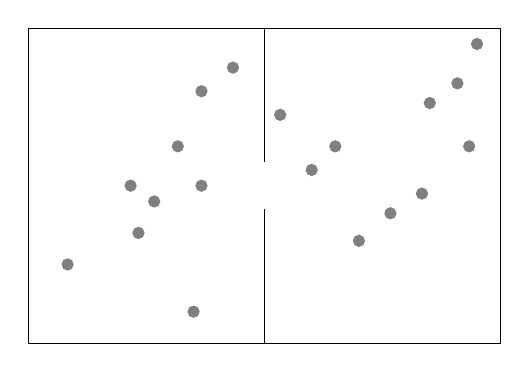
\begin{tikzpicture}
		\draw (0,0) -- (6,0) -- (6,4) -- (0,4) -- (0,0);
		\draw (3,0) -- (3,1.7);
		\draw (3,2.3) -- (3,4);
		
		\filldraw [gray] (0.5,1) circle (2pt);
		\filldraw [gray] (2.2,2) circle (2pt);		
		\filldraw [gray] (1.4,1.4) circle (2pt);
		\filldraw [gray] (2.6,3.5) circle (2pt);
		\filldraw [gray] (1.9,2.5) circle (2pt);
		\filldraw [gray] (2.1,0.4) circle (2pt);
		\filldraw [gray] (1.3,2) circle (2pt);
		\filldraw [gray] (2.2,3.2) circle (2pt);
		\filldraw [gray] (1.6,1.8) circle (2pt);
		%\filldraw [gray] (0.6,2.8) circle (2pt);
		
		\filldraw [gray] (4.2,1.3) circle (2pt);
		\filldraw [gray] (5.6,2.5) circle (2pt);
		\filldraw [gray] (4.6,1.65) circle (2pt);
		\filldraw [gray] (5.1,3.05) circle (2pt);
		\filldraw [gray] (3.2,2.9) circle (2pt);
		\filldraw [gray] (5,1.9) circle (2pt);
		\filldraw [gray] (3.6,2.2) circle (2pt);
		\filldraw [gray] (5.45,3.3) circle (2pt);
		\filldraw [gray] (3.9,2.5) circle (2pt);
		\filldraw [gray] (5.7,3.8) circle (2pt);
		
	\end{tikzpicture}
		
	Le probabilità che una particella vada a destra o a sinistra sono rispettivamente:
	$$ p_{s,s+1} = \frac{N-s}{N} $$
	$$ p_{s,s-1} ??? $$ %TODO
	
\end{multicols}

\subsection{Modello di Bernoulli-Laplace}

Descrive l'evoluzione di un gas; in questo caso abbiamo 2 gas diversi, A e B, ed $ N $ particelle del gas A e altrettante del gas B.

\begin{center}
	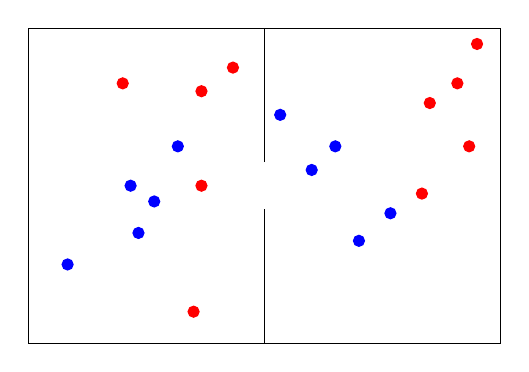
\begin{tikzpicture}
		\draw (0,0) -- (6,0) -- (6,4) -- (0,4) -- (0,0);
		\draw (3,0) -- (3,1.7);
		\draw (3,2.3) -- (3,4);
		
		\filldraw [blue] (0.5,1) circle (2pt);
		\filldraw [red] (2.2,2) circle (2pt);		
		\filldraw [blue] (1.4,1.4) circle (2pt);
		\filldraw [red] (2.6,3.5) circle (2pt);
		\filldraw [blue] (1.9,2.5) circle (2pt);
		\filldraw [red] (2.1,0.4) circle (2pt);
		\filldraw [blue] (1.3,2) circle (2pt);
		\filldraw [red] (2.2,3.2) circle (2pt);
		\filldraw [blue] (1.6,1.8) circle (2pt);
		\filldraw [red] (1.2,3.3) circle (2pt);
		
		\filldraw [blue] (4.2,1.3) circle (2pt);
		\filldraw [red] (5.6,2.5) circle (2pt);
		\filldraw [blue] (4.6,1.65) circle (2pt);
		\filldraw [red] (5.1,3.05) circle (2pt);
		\filldraw [blue] (3.2,2.9) circle (2pt);
		\filldraw [red] (5,1.9) circle (2pt);
		\filldraw [blue] (3.6,2.2) circle (2pt);
		\filldraw [red] (5.45,3.3) circle (2pt);
		\filldraw [blue] (3.9,2.5) circle (2pt);
		\filldraw [red](5.7,3.8) circle (2pt);
	
	\end{tikzpicture}
\end{center}

Supponiamo che in ogni istante sia scelta a caso una particella nel contenitore sinistro, una a caso nel contenitore destro e vengano scambiate. 

Lo stato $ S = \{0, 1, ..., N\} $ rappresenta il numero di palline di gas A a sinistra. 

$ p_{s,s} $ è la probabilità che ci siano $ n $ particelle A a sinistra e che dopo lo scambio questo valore rimanga invariato; questo può capitare se scambiamo una particella di A a sinistra con un'altra particella, sempre di A, a destra (oppure se scegliamo due particelle di tipo B).

$ p_{s,s} = ??? $ %TODO

$ p_{s,s-1} = \frac{s}{N}\cdot \frac{s}{N} = \frac{s^2}{N^2} ???$ %TODO

\section{Classificazione degli stati}

Due stati $ s $ e $ s' $ si dicono \textbf{comunicanti} quando $ s $ comunica con $ s' $, ovvero la probabilità di andare da $ s $ a $ s' $ è positiva:

$ p^{n}_{s,s'} = 0 $

$ p^{(???)}_{s,s'} = 0 $, con $ s' \ne s $ %TODO

Uno stato comunica con sè stesso. 

\paragraph{Definizione} (più precisa) Uno stato $ s $ comunica con uno stato $ s' $ se esiste $ n $ tale che la successione da $ s $ a $ s' $ in $ n $ passi è sempre positiva ??? %TODO

\paragraph{Proprietà} Siano $ s $ e $ s' $ due stati comunicanti: $ s \prec s' $

Se $ us < s' $ e $ s' < s'' $ %TODO controlla abbia senso (riguarda lezione)
, allora $ s \prec s'' $ \\
\\
In generale, se ho due cammini:

$ s, s_1, ..., s_{n-1}, s'' $

$ s', \bar{s}_1, ..., \bar{s}_{m-1}, s'' $
\\
Allora possiamo metterli insieme e fare un cammino che colleghi $ s, s''$. \\
\\
\\
Partendo dalla nozione di comunicazione possiamo definire una \textbf{relazione di equivalenza}. Nota: la comunicazione non è simmetrica. 

$ s \simeq s' $ se $ s \prec s' $ e $ s' \prec s $
\\
$ s \prec s $ perché lo stato comunica sempre con sè stesso.

Proprietà transitiva: se $ s \simeq s' $ e $ s' \simeq s'' $, allora $ s' \simeq s'' $

Proprietà simmetrica: $ s \simeq s' $ e $ s' \simeq s $
\\
\\
Abbiamo una relazione di equivalenza, possiamo definire una classe di equivalenza:
$$ [s] = \{s' | s' \simeq s\} $$

La nozione di comunicazione si può estendere alle classi di equivalenza:
$$ [s] \prec [s'] \text{ se } s \prec s'$$

Una classe equivalente ad $ s $ si dice \textbf{massimale} se non comunica con un'altra classe di equivalenza. 

Quando la catena di Markov arriva in uno stato che appartiene ad una classe massimale, rimane "bloccata" sempre dentro stati di quella classe. 

Una catena di Markov si dice \textbf{irriducibile} se da una sola classe di equivalenza ??? %TODO

cioè lo spazio degli eventi $ S $ è una sola classe di equivalenza.
\\
\\
Consideriamo la passeggiata aleatoria su $ [a,b] \subset \mathbb{Z} $ con condizioni assorbenti:

$$ a < s < b \qquad \qquad \begin{array}{c}
 	p_{s,s+1} = p \\
    p_{s,s-1} = 1-p
\end{array}$$

$$ \begin{array}{cc}
	p_{a,a} = 1 & p_{a,s} = 0 \\
	p_{b,b} = 1 & p_{b,s} = 0
\end{array}$$

Ovvero, se partiamo da uno stato interno lo spostamento è "normale", mentre se siamo in $ a $ o $ b $ rimaniamo sempre in quello stato (come ad esempio nella rovina dei giocatori). 

\paragraph{Esempio} Definiamo ora 3 classi di equivalenza:
$$ c_1 = \{a\} \quad c_2 = \{a+1, ..., b-1\} \quad c_3 = \{b\}, \qquad c_2 \prec c_1, c_2 \prec c_3$$ 

$ c_1 $ e $ c_3 $ sono massimali. In questo caso la catena di Markov non è irriducibile (il modello di Bernoulli-Laplace è un esempio di catena irriducibile). 

\paragraph{Periodo} Dato uno stato $ s \in S $:

$$ A^+_s = \{? | p_{s,s}^{(n)} > 0\} $$ %TODO
$$ A^+_s \ne 0 $$

Se $ n_1 \in A^+_s $ e $ n_2 \in A^+_s $, allora $ n_1 + n_2 \in A^+_s $

(ovvero la probabilità di andare dallo stato $ s $ allo stato $ s $ in $ n_1 + n_2 $ passi è positiva).

Il \textbf{periodo} di $ s $ (con $ A^+_s \ne 0 $) è:
$$ q = \text{MCD}(A^+_s) $$\\
\\
\\
In una \textbf{passeggiata aleatoria con condizioni periodiche} possiamo fare un movimento in senso orario o antiorario (dallo stato $ b $ torniamo ad $ a $). Non è detto che tutti gli $ A^+ $ siano divisibili per 2: il numero degli stati può essere dispari. 

Se $ q = 1 $, $ s $ si dice aperiodico. 

\paragraph{Osservazione} due stati equivalenti hanno lo stesso periodo.

Se $ s \simeq s' $, allora $ s \prec s' $; infatti, 

$ \exists \; n_1 : p_{s,s'}^{(n_1)} > 0 $

$ \exists \; n_2 : p_{s',s}^{(n_2)} > 0 $

Supponiamo $ q $ periodo di $ s $ e $ q' $ periodo si $ s' $. Vogliamo mostrare che $ q = q' $

Osserviamo che $ n_1 + n_2 $ è divisibile sia per $ q $, sia per $ q' $:
$$ p_{s,s}^{(n_1 + n_2)} > 0 \qquad \qquad \qquad p_{s',s'}^{(n_1 + n_2)} > 0  $$

Prendiamo un $ n \in A^+_s $:

$$ n + n_1 + n_2 \in A^+_s $$

$ n + n_1 + n_2 $ è divisibile per $ q' \Rightarrow n$ è divisibile per $ q' $.

Viceversa, preso $ n' \in A^+_{s'} $, $ n' $ è divisibile per $ q $.

???%TODO

Il periodo è una caratteristica delle classi di equivalenza. \\
\\
\\
Supponiamo di avere una passeggiata aleatoria su $ \mathbb{Z} $ (che è una catena di Markov irriducibile). Il periodo di ogni stato è 2:
$$ \mathbb{Z} = 2\mathbb{Z} \; \dot\bigcup \; 2\mathbb{Z} + 1$$

(dove $ \dot\cup $ è l'unione disgiunta).

La passeggiata aleatoria passa da un elemento di $ 2\mathbb{Z} $ ad un elemento di $ 2\mathbb{Z} + 1 $:

\begin{center}	
	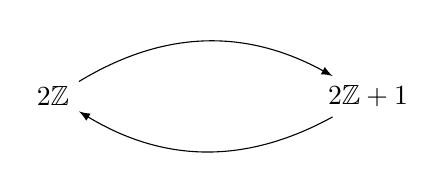
\begin{tikzpicture}[node distance=2cm, main/.style = {}]
	\tikzset{edge/.style = {->,> = latex}}
	
		\node[main] (1) [] {};
		\node[main] (2) [left of=1] {$ 2\mathbb{Z} $};
		\node[main] (3) [right of=1] {$ 2\mathbb{Z} + 1 $};
		
		\draw[edge] (2) to[bend left] (3);
		\draw[edge] (3) to[bend left] (2);
	\end{tikzpicture}
\end{center}

In generale, una classe di equivalenza $ C $ con periodo $ q > 1 $ può essere suddivisa in q sottoinsiemi:
$$ C = C_0 \dot\cup C_1 \dot\cup ... \dot\cup C_{q-1} $$

\begin{center}	
	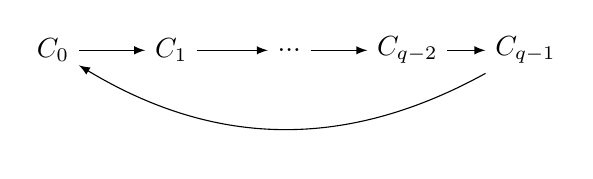
\begin{tikzpicture}[node distance=1.5cm, main/.style = {}, edge/.style = {->,> = latex}]

	
	\node[main] (1) [] {$ C_0 $};
	\node[main] (2) [right of=1] {$ C_1 $};
	\node[main] (3) [right of=2] {$ ... $};
	\node[main] (4) [right of=3] {$ C_{q-2} $};
	\node[main] (5) [right of=4] {$ C_{q-1} $};
	
	\path[edge]
	(1) edge node[] {} (2)
	(2) edge node[] {} (3)
	(3) edge node[] {} (4)
	(4) edge node[] {} (5)

	(5) edge[bend left] node[] {} (1);

	\end{tikzpicture}
\end{center}

E la catena di Markov percorre in maniera ciclica le classi. 

\subsection{Ricorrenza}
Vediamo ora un altro tipo di classificazione, detto appunto \textbf{ricorrenza}: questa è la proprietà di uno stato di ritornare (infinite) volte nella catena di Markov.

Definiamo, dati due stati $ s $ e $ s' $ e dato $ n > 0 $:

$$ f^{(n)}_{s,s'} = P(x_n = s', x_{n-1} \ne s', ..., x_n \ne s' | x_0 = s)$$

Questa è la probabilità di passare da $ s $ a $ s' $ per la prima volta in un tempo $ n $. 

Osserviamo che se consideriamo questi eventi per un dato $ n $ e per un $ n' \ne $, questi eventi sono incompatibili: se partendo da $ s $ arriviamo per la prima volta a $ s' $ in un tempo $ n $, ovviamente è impossibile che succeda la stessa cosa per un tempo $ n' \ne n $. 
In particolare, se facciamo la somma di queste probabilità, troveremo che questa è pari alla probabilità di uno di questi eventi:
$$ \sum_{n} f_{s,s'}^{(n)} = f_{s,s'} $$
è appunto la probabilità che si verifichi uno di quegli eventi, o in altre parole che arriveremo in uno stato $ s' $ partendo da uno stato $ s $ in un certo tempo. 

Consideriamo il caso $ s' = s $; in questo caso scriveremo per semplicità $ f_{s,s} = f_s $ e indica la probabilità di tornare, nel futuro, a $ s $. 

$ s $ è uno stato \textbf{ricorrente} se $ f_s $ = 1 (torniamo almeno una volta - in realtà infinite);

$ s $ è uno stato \textbf{transiente} se $ f_s < 1 $.

La probabilità di tornare infinite volte in uno stato ricorrente è 1. La probabilità di tornare almeno 2 volte in uno transiente è $ f_s^2 $; la probabilità di tornare almeno $ n $ volte è $ f_s^n $.

Negli stati transienti, la probabilità di tornare infinite volte invece è 0. La catena di Markov passa per gli stati transienti con probabilità 1 un numero finito di volte. 

\paragraph{Esempio: passeggiata aleatoria simmetrica}

La probabilità di tornare a 0 dopo $ 2n $ passi, oppure la probabilità che la passeggiata sia diversa da 0 per $ 2n $ passi si indica con la stessa quantità:

$$ P(x_{2n} \ne 0, x_{2n-1} \ne 0, ..., x_{1} \ne 0 | x_0 = 0) = u_{2n} = \binom{2n}{n}\frac{1}{2^{2n}}$$

$$u_{2n} \overset{ \text{per Stirling} }{\simeq} \frac{1}{\sqrt{\pi n}} \underset{n \to \infty}{\longrightarrow} 0$$

0 quindi è uno stato ricorrente per la passeggiata aleatoria simmetrica. 

Ad esempio, se consideriamo i soliti due giocatori che usano una moneta simmetrica, la probabilità che il guadagno non arrivi mai al pareggio è pari a 0. 

\subsection{Verificare se uno stato è transiente o ricorrente}
C'è una proprietà che semplifica il verificare se uno stato è transiente o ricorrente:

$ s $ è ricorrente se e solo se:
$$ \sum_{n=0}^{\infty} p_{s,s}^{n} = \infty $$
$ s $ è transiente se e solo se:
$$ \sum_{n=0}^{\infty} p_{s,s}^{n} < \infty \qquad \text{(la serie è convergente) } $$

\paragraph{Esempio} Applichiamo il metodo appena esposto considerando per esempio una passeggiata aleatoria su $ \mathbb{Z} $.
$$ p = \frac{1}{2} \qquad p_{0,0}^{(2n)} = u_{2n} = \binom{2n}{n}\frac{1}{2^{2n}} \simeq \frac{1}{\sqrt{\pi n}} $$

$$ \sum_{n=0}^{\infty} p_{0,0}^{(n)} = +\infty $$
Dobbiamo considerare la serie $\frac{1}{\sqrt{n}}$ che è divergente per $ n \ge \frac{1}{2} $ e converge per $ n < \frac{1}{2} $. In questo caso è divergente. 

$$ p \ne \frac{1}{2} \qquad p_{0,0}^{(2n)} = \binom{2n}{n} p^n (1-p)^n = \underbrace{\binom{2n}{n}\frac{1}{2^2n}}_{\displaystyle = u_{2n} \simeq \frac{1}{\sqrt{\pi n}}} \cdot \; \underbrace{2^{2n} p^n(1-p^n) }_{\displaystyle = 4p(1-p^n)} $$

Consideriamo la funzione $ p(1-p) $:

$$ \frac{\partial}{\partial{p}} p(1-p) = 1.p -p = 1 - 2p $$
È positiva per $ p < \frac{1}{2} $ e negativa per $ p > \frac{1}{2} $.

\begin{multicols}{2}
	\begin{tikzpicture}
		\begin{axis}[axis lines=left, xtick={0,1}, ytick={0.25}, ymax=0.3, xmax=1.1, width=7cm]
			\addplot [
			domain=0:1, 
			samples=100, 
			color=black,
			]
			{x*(1-x)};
		\end{axis}
	\end{tikzpicture}
	
	Questa quantità: $ (4p(1-p))^n $ è sempre minore di 1. È una serie geometrica convergente; allora, in questo caso lo stato 0 è transiente. 
\end{multicols}

Quindi nel caso di passeggiata aleatoria non simmetrica i due giocatori andranno in pareggio solo un numero finito di volte. 

Verifichiamo ora la seconda proprietà, quella che ci permette di determinare se uno stato è transiente. Introduciamo la \textbf{funzione generatrice}. È uno strumento che si usa in molti casi, quando abbiamo una successione. 

\begin{align*}
	& f_{s,s}^{(0)} \\
	U(z) & = \sum_{n=0}^{\infty} p_{s,s}^{(n)} z^n \\
	& |z| < 1 \\
	F(z) & = \sum_{n=1}^{\infty} f_{s,s}^{(n)} z^n
\end{align*}

Osserviamo che $ U(z) = 1 + F(z)\cdot U(z) $. Si vede dall'equazione del rinnovamento. 

La probabilità di tornare a $ s $ dopo $ n $ passi è:
$$ p_{s,s}^{(n)} = \sum_{k=1}^{n} f_{s,s}^{(k)} p_{s,s}^{(n-k)} \qquad \text{con } n \ge 1 $$
C'è quindi una prima volta dove arriviamo a $ s $ ($ f_{s,s}^{(k)} $) e poi ci torniamo una seconda volta (al tempo $ n-k $). 

Per Markov è come se la catena ripartisse dall'inizio. 


 $$ U(z) = \sum_{n=0}^{\infty} p_{s,s}^{(n)} z^n $$
 
Per $ n = 0, p_{s,s}^0 = 1 $ quindi 

$$ U(z)	= 1 + \sum_{n=1}^{n} (\sum_{k=1}^{n} f_{s,s}^{(k)} p_{s,s}^{(n-k)}) z^n $$

Introduciamo $ m = n-k \Rightarrow n=m+k $

\begin{align*}
	U(z) & = 1 + \sum_{m=0}^{\infty} \sum_{k=1}^{\infty} f_{s,s}^{(k)} p_{s,s}^{(m)} \equalto{z^{m+k}}{z^m\cdot z^k} \\
	& = 1 + (\sum_{m=0}^{\infty}p_{s,s}^{(m)} z^m )(\sum_{k=1}^{\infty} f_{s,s}^{(k)}z^k ) \\
	& = 1 + F(z)\cdot U(z) \\
	\lim\limits_{z \uparrow 1} \sum_{n=1}^{\infty} f_{s,s}^{(n)} z^n & = \sum_{n=1}^{\infty} f_{s,s}^{(n)} = f_s \\
	\lim\limits_{z \uparrow 1} U(z) & = \sum_{n=0}^{\infty} p_{s,s}^{(n)} \\
	U(z) & = \frac{1}{1 - F(z)}
\end{align*}

Nel caso del periodo abbiamo che due stati con la stessa classe di equivalenza hanno lo stesso periodo. Anche la ricorrenza/transienza hanno la stessa proprietà (ovvero, due classi di equivalenza hanno la stessa ricorrenza/transienza). 

\paragraph{Lemma} Dato uno stato $ s $ ricorrente, se $ s \prec s' $ allora $ s' \prec s $.

Supponiamo per assurdo $ s' \nprec s $.

$ \exists n_1 : p_{s,s'}^{(n_1)} > 0$.

Quindi posso tornare un numero finito di volte su $ s $. Ma se uno stato è ricorrente, posso tornare infinite volte in uno stato. ASSURDO
Quindi $ s' \approx s $

\paragraph{Lemma} Se $ s \approx s' $ e $ s $ è ricorrente, allora $ s' $ è ricorrente. 

Questo lemma ci dice che una classe di equivalenza ha tutti stati ricorrenti, oppure tutti stati transienti. 

Supponiamo $ s $ ricorrente; supponiamo $ s \approx s' $. Quindi $ s \prec s' $ e $ s' \prec s $. 

$$ \Rightarrow \exists n_1 : P_{s,s'}^{(n_1)} > 0 \land \exists n_2 : p_{s,s'}^{(n_2)} > 0 $$

$$ \sum_{n=0}^{\infty} p_{s',s'}^{(n)} \ge \sum_{n = n_1 + n_2}^{\infty} p_{s',s'}^{(n)} $$ 

Se invece di partire da $ n = 0 $ partiamo da $ n = n_1+n_2 $, come facciamo ad andare da $ s' $ a $ s' $? Andiamo in $ n_2 $ da $ s' $ a $ n $, e in $ n - n_1 - n_2 $ possiamo andare a $ s $, e infine in $ n_1 $ da $ s $ a $ s' $:

$$ \ge \sum_{n=n_1+n_2}^{\infty} p_{s',s}^{(n_2)} p_{s,s}^{(n-n_1-n_2)} p_{s,s'}^{(n_1)} $$
Sia $ k = n-n_1-n_2 $:
$$ = p_{s',s}^{n_2} p_{s,s'}^{(n_1)} \sum_{k=0}^{\infty} p_{s,s}^{(k)} = +\infty$$

$$ \Rightarrow s' \text{ è ricorrente.} \qed $$

\section{Teorema ergodico per catene di Markov}
Questo risultato riguarda le catene di Markov con una sola classe di equivalenza con stati ricorrenti e aperiodica. Possiamo dimostrare il teorema ergodico per catene di Markov. 

Formalmente, 
$$ 
\begin{array}{cc}
	s \in S & v_s = \sum_{n=1}^{\infty} n f_{s,s}^{(n)} \text{ (attesa del tempo di ritorno)} \\
	s \text{ ricorrente } & f_s = \sum_{n=1}^{\infty} f_{s,s}^{(n)} = 1 \\  
\end{array} $$

$$ p_{s,s'}^{(n)} \underset{n \to \infty}{\longrightarrow} \frac{1}{v_s} $$
$$ \text{se } v_s = +\infty, \; \; \frac{1}{v_s} = 0 $$

Se $ v_s = +\infty $ allora non è necessario che sia aperiodica. 

Questo teorema (che non dimostreremo) è interessante perché ci dice che quando abbiamo una sola classe di equivalenza aperiodica con gli stati ricorrenti, è come se la catena di Markov si dimenticasse del punto di partenza: quando faccio tendere $ n $ all'infinito, la probabilità di andare da uno stato qualunque a $ s $ tende ad un limite che non dipende dal punto di partenza.

Si può anche vedere che facendo andare avanti la catena di Markov e contando quante volte passa per $ s $, la frequenza/percentuale di tempo tende a questo limite. 

È come nel caso dello schema di Bernoulli; per la legge dei grandi numeri, se contiamo quante volte otteniamo il successo, questa quantità tende alla probabilità. La probabilità ha il significato di frequenza.

Anche nelle catene di Markov che sono dipendenti, nel caso ergodico la probabilità di andare da uno stato ad un altro tende ad un certo limite che è anche la frequenza con cui la catena di Markov passa per quello stato. 

Questo valore è l'attesa del tempo di ritorno; c'è però un metodo più semplice per calcolarlo. 

Supponiamo nel caso finito che uno stato sia ricorrente, ci sia una sola classe di di equivalenza (e quindi tutti gli stati sono ricorrenti) e aperiodici. 
\\ \\
Sappiamo che $ p_{s',s}^{(n)} \to v_s^{-1} = u_s $.
\\ \\
Osservazione: $ p_{s',s}^{(n+1)} = \sum_{s''} p_{s',s''}^{(n)} p_{s'',s} $

$$ \begin{array}{cc}
	p_{s,s'}^{(n+1)} \underset{n \to \infty}{u_s} & \sum_{s''}p_{s',s''}^{(n)} p_{s'',s} \\ 
	
	u_s = \sum_{s''} u_{s''} & \sum_{s \in S} u_s = 1
\end{array} $$

$ u_s $ è una distribuzione di probabilità sugli stati;

$$ \sum_{s \in S} p_{s'', s}^{(n)} = 1 \qquad \forall s \in S $$

$$ u_s = \sum_{s''} u_{s''}p_{s'',s}$$

Ho un sistema di equazioni lineari: abbiamo $ k $ incognite (gli stati) e $ k+1 $ equazioni. Ma le equazioni $ \sum_{s''} p_{s'', s}  \forall s \in S$ non sono linearmente indipendenti, quindi ne posso prendere solo una. Il mio sistema diventa:

$$ 
\begin{cases} \sum u_s = 1 \\ u_s = \sum_{s''} u_{s''}p_{s'',s} \forall s \in S \end{cases} 
$$

Supponiamo ora:

$$ \sum_{s \in S} v_s = 1 \qquad \qquad \qquad v_s = \sum_{s''} v_{s''}p_{s'',s} $$

Con $ S $ finito. C'è un'unica soluzione:

\begin{align*}
	v_s & = \sum_{s''}v_{s''}p_{s'',s}^{(n)} \\
	 \text{Faccio } & \text{tendere } n \text{ all'infinito: }\\
	& = \sum_{s''}v_{s''}u_s = u_s
\end{align*}

Nell'equazione $ \sum_{s''}v_{s''}u_s $ posso portare fuori $ u_s $ perché non dipende dalla sommatoria; ma la sommatoria è uguale a 1, quindi ottengo proprio $ u_s $.

\vspace{1cm}
\hrule 
\vspace{1cm}

Ripetiamo l'enunciato del teorema ergodico per le catene di Markov: supponiamo di avere una catena di Markov con spazio egli stati $ S $, con una sola classe di equivalenza e stati ricorrenti. La proprietà di ricorrenza sappiamo valere per tutti gli elementi di una classe di equivalenza. Siano inoltre gli stati aperiodici (e anche questa è una proprietà che vale per tutti gli stati di una classe di equivalenza).

Dato uno stato $ s $, definiamo:

$$ \mu_s = \sum_{n=1}^{\infty} n \cdot f_s^{(n)} $$

Come interpretiamo $ \mu_s $? Siccome gli stati sono ricorrenti, sappiamo che partendo da uno stato, ci ritorniamo con probabilità 1; possiamo allora considerare il tempo di ritorno come una variabile aleatoria detta, appunto, \textit{tempo di ritorno}. $ \mu_s $ è l'attesa del tempo di ritorno. 

Allora 
$$ p_{s,s'}^{(n)} \to \ddfrac{1}{\mu_s} $$

Questa quantità è uguale a 0 se $ \mu = +\infty $. Se $ \mu= +\infty $, non è necessaria aperiodicità. 

Nel caso $ S $ finito, detto $ u_s = \ddfrac{1}{\mu_s} $
$$ \qquad \displaystyle \sum_{s \in S} u_s = 1 $$
e
$$ \forall s' \qquad \sum_{s} u_s p_{s,s'} = u_s'$$

Queste relazioni ci dicono che $ u_s $ è una distribuzione invariante o stazionaria, ovvero se $ u_s $ soddisfa le due equazioni e mettiamo $ u_s $ come distribuzione iniziale in una catena di Markov, vediamo che nei tempi successivi rimane invariante (ovvero la distribuzione rimane $ u_s $)Se $ u_s $ è la distribuzione iniziale, da $ \sum_{s} u_s p_{s,s'} = u_s' $ segue che $ u_s $ è anche la distribuzione al tempo 1. È anche stazionaria perché non cambia nel tempo

Vogliamo verificare se la proprietà sia vera anche nel caso $ S $ infinito. 

Dato $ \bar{s} \in S $,

$$ p_{\bar{s},s'}^{(n+1)} = \sum_{s \in S} p_{\bar{s}, s}^{(n)} p_{s,s'} $$


Questa è una serie, dobbiamo passare al limite. Nel caso infinito però non è sempre vero che il limite della serie è uguale alla serie dei limiti. Consideriamo $ \bar{S} \subset S $ finito anziché $ S $:

\begin{align*}
	p_{\bar{s}, s'}^{(n+1)} & \ge \sum_{s \in \bar{S} } p_{\bar{s},s}^{(n)} p_{s,s'} \qquad \text { per il teorema ergodico} \\
	u_{s'} & \ge \sum_{s \in \bar{S}} u_s p_{s,s'} \\
	u_{s'} & \ge \sum_{s \in S} u_sp_{s,s'} \qquad \text{(I)}
\end{align*}

Abbiamo dimostrato una disuguaglianza. Definiamo 
$$ 0 < \alpha = \sum_{s \in S} u_s \le 1 \qquad \text{(II)} $$
$\alpha > 0$ perché gli $ u_s > 0$, ma $ \alpha \le 1$ perché $ \sum_{s' \in S} p_{s,s'}^{(n)} = 1 $

Dobbiamo dimostrare che in (I) c'è uguaglianza, e in (II) che la somma è pari a 1.

Supponiamo per assurdo che non ci sia uguaglianza in (I) per un particolare stato $\bar{s}'$:

$$ u_{\bar{s}'} > \sum_{s \in S} u_s p{s,s'} $$

Allora quando sommiamo tutti gli stati, avremo la disuguaglianza stretta:
$$ \sum_{s'} u_{s'} > \sum_{s'} \sum_{s} u_s p_{s,s'} $$
$$ \alpha = \sum_{s'} u_{s'} > \sum_{s'} \sum{s} u_s p_{s,s'}$$
$$ \alpha > \alpha \text{ ASSURDO } $$

Quindi anche nel caso infinito, $ u_s $ è una distribuzione di probabilità, cioè la somma è pari a 1:

\begin{align*}
	u_{s'} & = \sum_{s} u_s p_{s,s'}^{(2)} \\
	u_{s'} & = \sum_{s} u_s p_{s,s'} ^{(n)}
\end{align*}

Per $ n \to \infty $, $ u_{s'} = \sum_{s} u_su_{s'}$
\begin{align*}
u_{s'} & = \alpha u_{s'} \qquad \qquad u_{s'} > 0 \\
& \Rightarrow \alpha = 1 \qed
\end{align*}

Abbiamo ipotizzato finora l'attesa di ritorno $\mu_s < +\infty$ (cioè $\mu_s$ finito).

Nel caso $\mu_s = + \infty$, allora $ p_{s,s'} \to 0 $. Lo abbiamo visto nel caso aperiodico, ma questa proprietà è vera anche nel caso generale. Questo ci porta a fare una classificazione degli stati ricorrenti in 2 categorie:

$$ \text{supponiamo } s \text{ ricorrente: } \begin{cases*}
	\mu_s < +\infty, & s \text{ ricorrente positivo} \\
	\mu_s = + \infty, & s \text{ricorrente nullo}
\end{cases*}$$

Nel primo caso quindi l'attesa del tempo di ritorno è finita, nel secondo infinita. 
\\
\\
Supponiamo di avere una classe di equivalenza $ S $ irriducibile e ricorrente. Vogliamo mostrare che non è possibile che ci sia uno stato ricorrente positivo e uno stato ricorrente nullo. Supponendo quindi che $ s_1 $ sia positivo, vogliamo mostrare che $ s_2 $ non può essere ricorrente nullo. 

Dato un $ s $,
$$ p_{s,s{_1}}^{(n)} \underset{n \to \infty}{\longrightarrow} u_{s_{1}} > 0$$

$$ \exists n_1 : p_{s_1, s_2}^{n_1} > 0 \qquad \text{perché } s_1, s_2 \in S  $$

Ma $ p_{s,s_2}^{(n)} > p_{s,s_1}^{(n - n_1)} p_{s,s_2}^{(n_1)} $

$ p_{s,s_2}^{(n)} $ non tende a 0 (per $ n \to \infty $)

$$ \Rightarrow s_2 \text{ è ricorrente positivo} \qed $$

Una conseguenza è che se $ S $ è finito, non ci sono stati ricorrenti nulli, perché abbiamo che $ \sum_{s' \in S} p_{s,s'}^{(n)} = 1 $.


Essendo S finito, possiamo passare al limite della somma. Se gli stati fossero ricorrenti nulli, il limite tenderebbe a 0, e siccome è una somma finita, anche la somma tenderebbe a 0. Ma la somma è pari a 1, quindi dev'esserci almeno uno stato ricorrente positivo. E abbiamo appena visto che se abbiamo una sola classe di equivalenza e uno stato è ricorrente positivo, allora sono tutti ricorrenti positivi - anche se la dimostrazione appena vista funziona solo nel caso aperiodico. 

Quindi in una tale catena di Markov (sola classe di equivalenza, irriducibile, stati ricorrenti positivi, aperiodica) abbiamo una distribuzione invariante, e le probabilità tendono a $ u_s $: ma come si fa a calcolare questo limite? La cosa più semplice è provare a risolvere il sistema d'equazioni.

Vediamo il caso più semplice di catena di Markov con spazio degli stati finiti, che è una catena di Markov con due stati: $ S = \{0,1\} $. La matrice di transizione è:

$$ \Pi = \left(\begin{matrix}
	p & 1-p \\
	1-q & q
	\end{matrix}\right)  \qquad \qquad 
	\begin{array}{c} 
		0 < p < 1 \\ 
		0 < q < 1 
	\end{array}
$$

\begin{enumerate}
	\item $ u_0 + u_1 = 1 \qquad \qquad $ (perché è una distribuzione di probabilità)
	\item $u_0 \cdot p + u_1 \cdot (1-q) = u_0 $
	\item $u_1 \cdot q + u_0 \cdot (1-p) = u_1 $
\end{enumerate}

2. e 3. sono uguali, possiamo usare 1. e 2. 
$$ \begin{cases*}
	u_0 = u_1\left(\ddfrac{1-q}{1-p}\right) \\
	u_1\ddfrac{1-q}{1-p} + u_1 = 1
\end{cases*}$$
$$  
	\begin{cases*}
		u_1 \ddfrac{(1-q)+(1+p)}{1-p} = 1 \\
		u_0 = u_1(\ddfrac{1-q}{1-p})
	\end{cases*}
	\qquad 
	\begin{cases*}
		u_0 = \ddfrac{1-q}{2-p-q} \\
		u_1 = \ddfrac{1-p}{2-p-q} 
	\end{cases*}
$$

Possiamo rappresentare la passeggiata aleatoria con un cerchio:

\begin{center}
	\begin{tikzpicture}[point/.style={inner sep=2pt, fill=black, circle}]
		%\draw[red, thick] (0,0) circle (2 cm);
		
		\node[point, label=0] (1) at (0,2) {};	
		\node[point, label=1] (2) at (1.5,1.5) {};	
		\node[point, label=2] (3) at (2,0) {};	
		\node[point, label=3] (4) at (1.3,-1.7) {};	
		\node[point, label=4] (5) at (-1.3,-1.7) {};	
		\node[point, label=...] (6) at (-2,0) {};	
		\node[point, label=$ r-1 $] (7) at (-1.5,1.5) {};	
		
		\path []
		(1) edge[bend left, ->] (2)
		(1) edge[bend right, ->] (7); 
		
		\node[] (8) at (6,1) {$ |S| = n $};
		
	\end{tikzpicture}	
\end{center}

Se $ r $ è dispari, la catena è aperiodica.

\begin{align*}
	& u_0 + u_1 + ... + u_{r-1} = 1 \\
	& 1 \le s \le r-2 \\
	u_s & = u_{s-1} p + u_{s+1}(1-p) \\
	u_0 & = u_{r-1}p + u_1(1-p) \\
	u_{r-1} & = u_{r-2} p + u_0(1-p)
\end{align*}

Abbiamo $ r+1 $ equazioni e $ r $ incognite. Possiamo però intuitivamente provare a vedere quale sarà la distribuzione invariante anche senza risolvere le equazioni: immaginiamo di fare andare avanti la passeggiata aleatoria per molto tempo, è naturale pensare che alla fine la distribuzione sia uniforme: se giriamo tanto a caso, la probabilità di trovarci in un qualsiasi punto sia uguale. Ipotizziamo quindi che $ u_s = \frac{1}{r} $. Sostituendolo nelle equazioni, in effetti vengono risolte. 

Questa è in realtà una distribuzione invariante anche nel caso pari, ma nel caso pari non è aperiodico, quindi non è vero che la distribuzione tende alla distribuzione uguale per tutti gli stati: se noi partiamo da 0, per tornare a 0, sia che facciamo lo stesso numero di passi orari e antiorari, oppure facciamo un certo numero di giri attorno, il tempo che impieghiamo è sempre pari, e quindi la probabilità di tornare a 0 dopo un tempo dispari è 0. 


Altri modelli che abbiamo visto sono i modelli di estrazione dall'urna: abbiamo visto il modello di Ehrenfest e di Laplace-Bernoulli. In entrambi i modelli abbiamo due urne. Nel primo scegliamo a caso una pallina e la spostiamo da un'urna all'altra; nel secondo, abbiamo $ n $ palline bianche e $ n $ palline nere. Di queste $ 2n $ palline, metà stanno nell'urna A e metà nell'urna B. Possiamo prendere come stato il numero delle palline bianche in A. Quello che osserviamo è che il modello di Ehrenfest non è aperiodico: come nel caso della passeggiata aleatoria ha periodo 2. 

Rappresentiamo gli stati come punti, mettendo una freccia per indicare le transizioni possibili. Il numero delle palline nell'urna A può aumentare o diminuire, ovvero possiamo fare un passo a destra o un passo a sinistra. Possiamo tornare solo nei tempi pari, e quindi in questo caso - siccome il periodo è 2 - non possiamo applicare direttamente il teorema ergodico. 

Nel modello di Laplace-Bernoulli il numero di palline bianche può anche rimanere invariato:

\begin{center}
	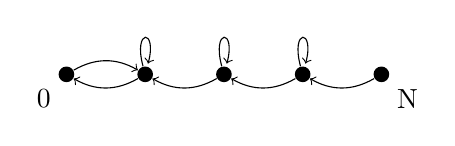
\begin{tikzpicture}[point/.style={circle, inner sep=2pt, fill=black}]
		\node[point, label=below left:0] (0) at (-2,0) {};
		\node[point] (1) at (-1,0) {};
		\node[point] (2) at (0,0) {};
		\node[point] (3) at (1,0) {};
		\node[point, label=below right:N] (4) at (2,0) {};
		
		\path[e/.style={bend left, ->}]
		(0) edge[e] (1)
		(1) edge[e] (0)
			edge[loop above] (1)
		(2) edge[e] (1)
			edge[loop above] (2)
		(3) edge[e] (2)
			edge[loop above] (3)
		(4)	edge[e]	(3);
		
	\end{tikzpicture}
\end{center}

se scambiamo 2 palline bianche tra le urne A e B, il numero delle palline bianche in A è invariato. Se la probabilità di rimanere nello stato è 0, allora il periodo deve essere 1  e possiamo usare il teorema ergodico. Intuitivamente, comunque, possiamo affermare che 

$$ u_s < \frac{\binom{N}{S}\binom{N}{N-S}}{\binom{2N}{N}} $$

e questa disuguaglianza dovrà soddisfare le equazioni. 

\paragraph{Teorema} Supponiamo S infinito, una sola classe di equivalenza aperiodica irriducibile. Supponiamo ci sia una distribuzione invariante $ u_s $, con $ 0 \le u_s \le 1 $:
$$ \sum_{s}u_s = 1 \qquad \forall s', u_{s'} = \sum_{s} u_s p_{s,s'} $$
Allora gli stati sono ricorrenti positivi. 
\\
\\
Dobbiamo far vedere che non sono ricorrenti nulli o transienti. Supponiamo per assurdo siano transienti.

La proprietà equivalente a essere transienti è la seguente:
$$ \sum_n p^{(n)}_{s,s} < + \infty $$ 
Questo implica in particolare che anche la probabilità di andare da uno stato qualunque, es. da $ s' $ a $ s $ con $ s' \ne s $ tende a 0:
$$ p_{s,s'} \underset{n\to \infty}{\longrightarrow} 0  $$
Possiamo scrivere l'equazione del rinnovamento; questa equazione deve tendere a 0::
$$ p_{s',s}^{(n)}  = \sum_{k=1}^{n} p^{(k)}_{s',s} p^{(n-k)}_{s,s} \underset{n \to \infty}{\longrightarrow} 0$$

Si può dividere in due parti:
$$ = \sum_{k=1}^{\frac{n}{2}} + \sum_{k=\frac{n}{2} + 1}^{n}$$
Si vede che non è possibile che esista una distribuzione invariante: se $ u_s $ è una distribuzione invariante, allora
$$ u_s = \sum_{s'}u_{s'} p_{s',s} $$
Ma questa si può iterare:
$$ = \sum_{s'}u_{s'} p^{(n)}_{s',s} $$
Se noi facciamo tendere $ n $ all'infinito, se $ s $ fosse uno stato transiente, la probabilità tenderebbe a 0; di conseguenza $ u_s = 0 $, e quindi $ u_s $ non sarebbe una distribuzione di probabilità.

Se gli stati fossero ricorrenti nulli, dal teorema ergodico abbiamo che $ p^{(n)}_{s',s} \to 1 $. Potremo usare lo stesso argomento. 

Quindi gli stati non possono essere ne transienti ne ricorrenti nulli: devono essere ricorrenti positivi. 

\section{Modello di coda}
In questo modello abbiamo dei clienti, che arrivano e vanno dagli sportelli dove vengono serviti. Il tempo che passano agli sportelli è aleatorio. Supponiamo che il tempo sia discreto. 

Uno sportello può contenere un cliente, gli altri clienti sono in coda. 

Definiamo $ p $ la \textbf{probabilità di arrivo di un cliente}, mentre $ q $ la probabilità di \textbf{fine del servizio}, $ 0 \le p \le 1 $ e $ 0 \le q \le 1 $. Gli arrivi dei clienti e la fine del servizio sono indipendenti. 

Questo è descritto da una catena di Markov in cui lo spazio degli stati è $ \mathbb{N} $: $ S = \mathbb{N} = \{0, 1, ...\} $, e ha una sola classe di equivalenza di periodo 1.

Ci chiediamo ora qual è la probabilità, partendo da 0, di rimanere nello stato 0 (ovvero che non ci sia nessun cliente e che non arrivi nessun cliente), e altre probabilità, con $ S = \mathbb{N} $:
$$ \begin{array}{ccc}
  p_{0,0} = 1-p & p_{1,1} = p\cdot q + (1-p) 1-q  & p_{1,2} = p(1-q) \\
  p_{0,1} = p & p_{1,0} = (1-p)q & 
\end{array} $$

$ p_{1,1} $ indica la probabilità che, dopo aver finito di servire un cliente ne arrivi uno nuovo; oppure di non finire di servire un cliente, e che non arrivi nessun nuovo cliente. 

In generale, per $ s \ge 1 $:
\begin{align*}
	p_{s,s} & = p\cdot q + (1-p) (1-q) & = r \\
	p_{s,s+1} & = p(1-q) & = d \\
	p_{s,s-1} & = q(1-p) & = l
\end{align*}

Questa passeggiata è ricorrente positiva? Se esiste una distribuzione invariante si, se non esiste o gli stati sono ricorrenti nulli oppure transienti. 

%2020-10-21

Vogliamo quindi vedere se gli stati sono ricorrenti o transienti, e nel primo caso se sono ricorrenti positivi o ricorrenti nulli. 

Vogliamo scrivere le equazioni per la distribuzione invariante. Definiamo $ u_i $ la distribuzione invariante, con $ i \in \mathbb{N} $:
\begin{align*}
	\sum_{i=0}^{\infty} u_i & = i \\
	u_0 & = u_0(1-p) + u_1 l \\
	u_1 & = u_0 p + u_1 r + u_r l \\
	u_s & = u_{s-1}d + u_s r + u_{s+1} l, \qquad \qquad s \ge 2 \\
	u_1 l & = u_0 p \\
	u_1(1-r-l) & = u_2 l \\
	u_1 d & = u_2 l \\	
	u_s d = u_{s+1} l
\end{align*}

Mettiamo insieme le equazioni:
$$ u_1 = u_0 \frac{p}{l} \qquad \qquad u_2 = u_1\frac{d}{l} \qquad \qquad u_{s+1} = u_s \frac{d}{l} $$
Riscritte in termini di $ u_0 $:
$$ u_2 = u_0 \frac{p}{l}\frac{d}{l} \qquad \qquad u_s = u_0 \frac{p}{l} \left(\frac{d}{l}\right)^{s-1} $$

Sapendo che $ \sum_{i=0}^{\infty} u_i = 1 $:

$$ u_0 \left( 1 + \frac{p}{l} + \frac{p}{l}\frac{d}{l} + \frac{p}{l} \left(\frac{d}{l}\right)^2 + ... \right) = 1 $$



L'equazione è possibile solo se questa serie:
$$ u_0 \left(1 + \frac{p}{l} \left( \sum_{j=0}^{\infty} \left(\frac{d}{l}\right)^j\right)\right) $$

è convergente; ma questa è una serie geometrica, ed è convergente per $ \frac{d}{l} < 1 $.

Andiamo a ricordare che cos'era $ d $:
$$ \begin{array}{cc}
d = p(1-q) & l = q(1-p) \end{array} $$

\begin{align}
	\frac{d}{l} < 1 & \Rightarrow d < l \\
	\Rightarrow & p(1-q) < q(1-p)
	\Rightarrow &	\frac{p}{1-p} < \frac{q}{1-q} % & p < q
\end{align}

Consideriamo ora la funzione $ \frac{x}{1-x} $; è una funzione strettamente crescente, quindi l'ultima disequazione scritta sopra è equivalente a
$$ p < q $$

Quindi la conclusione perché esista la distribuzione invariante è proprio $ p < q $. Se esiste la distribuzione invariante, gli stati sono \textbf{ricorrenti positivi}. 


Intuitivamente, essendo $ p $ è la probabilità di arrivo di un cliente e $ q $ la probabilità che un cliente vada via, se $ p < q $ l'afflusso dei clienti è minore della tendenza dei clienti a lasciare il sistema; questo fa sì che non si formi una coda lunga, perché il flusso degli arrivi è più piccolo del flusso delle partenze, e gli stati sono appunto ricorrenti positivi. 

Rimane da vedere il caso $ p \ge q $; ci sono due possibilità: gli stati sono \textbf{ricorrenti nulli} oppure \textbf{transienti}. 

Ci possiamo ricondurre al problema della rovina del giocatore: in quel caso è una passeggiata aleatoria in cui possiamo aumentare o diminuire di 1. Qui però c'è anche la possibilità di rimanere nello stesso stato all'istante successivo. 
Ma possiamo trascurare questi tempi e considerare solo quelli in cui c'è un cambiamento di stato per ricondurci al problema della rovina del giocatore. Partendo da uno stato, vogliamo calcolare la probabilità di andare a destra o a sinistra nel caso non rimaniamo nello stesso stato. Nel caso $ s \ge 1 $, definiamo $ \bar{p} $ la probabilità di andare nello stato successivo se non rimaniamo nello stesso stato:

$$ \bar{p}=\bar{p}_{s, s+1} = \frac{d}{1-r}$$

nel modello di coda questa probabilità è uguale a $ d $, ma condizioniamo al fatto di non rimanere nello stesso stato. Analogamente:
$$ 1-\bar{p}= \frac{l}{1-r} = \bar{p}_{s,s-1} $$
E nel caso dello zero:

$$ \bar{p}_{0,1} = 1 $$

Perché se partiamo dallo stato 0 e sappiamo che non rimaniamo nello stato, con probabilità 1 andiamo nello stato 1.

\begin{multicols}{2}
	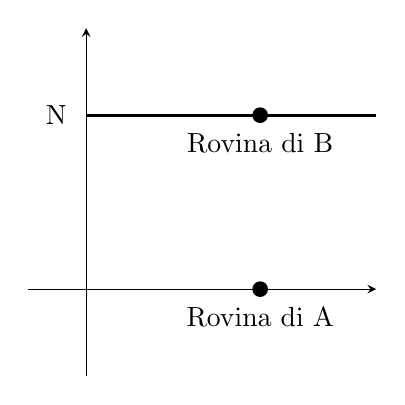
\begin{tikzpicture}
		\begin{axis}[axis lines = middle, ticks=none, width=6cm, height=6cm, ymin=-1, ymax=3, xmin=-1]
			\node[color=black, fill, circle, inner sep=2pt, label=below:{Rovina di A}] at (axis cs:3,0) {};
			\node[color=black, fill, circle, inner sep=2pt, label=below:{Rovina di B}] at (axis cs:3,2) {};
			\node[label=left:{N}] at (axis cs:0,2) {};
			\addplot[color=black, very thick, domain=0:5, samples=2]	
			{0*x + 2}; 
		\end{axis}
	\end{tikzpicture}
	\\
	\\
	Probabilità di rovina partendo da $S = 1- \frac{S}{N} $\\ 
	\\
	\\
	La probabilità tende a 1 per $ N \to \infty $
\end{multicols}

Quindi, se $ S = 1 $, siccome andremo a 0, dovremo per forza ripassar e per 1; gli stati sono ricorrenti. Inoltre sono ricorrenti nulli perché non c'è distribuzione di probabilità invariante . 

L'interpretazione è che la coda è lunga, ma ogni tanto si svuota. 
\\
\\
Un altro caso possibile è $ p = q $; in questo caso $ d = l $ e si ha che $ \bar{p} = \frac{1}{2} $. Nel caso della rovina del giocatore, quando le due probabilità sono uguali, la rovina del primo giocatore si ha quando si torna allo stato 0; questo implica che lo stato 0 è ricorrente. Sappiamo già però che non può essere ricorrente positivo (lo è nel caso $ p < q $); gli stati allora devono essere necessariamente ricorrenti nulli. 

Se $ p > q $, è come la passeggiata asimmetrica: $ d = \frac{p}{1-p} > l = \frac{q}{1-q} $ e $ \bar{p} > \frac{1}{2} $: la probabilità di andare a destra è maggiore della probabilità di andare a sinistra. C'è una probabilità positiva che il primo giocatore non si rovini, quindi che non torni a 0. Quindi in questo caso gli stati sono transienti. L'interpretazione quindi è che lo sportello si può vuotare un numero finito di volte, prima di allungarsi e non riuscire più a svuotarsi. 

\section{Reversibilità}
È una proprietà che possono possedere le catene di Markov. 

Supponiamo di avere una catena irriducibile ergodica aperiodica. Sia $ S $ il suo spazio degli stati; abbiamo una distribuzione invariante $ u_s $. Nella catena di Markov, la distribuzione di probabilità è $ X_0, X_1, X_2, ... $.

Se come distribuzione iniziale diamo $ u_s $, ai tempi successivi la distribuzione di $ X_1, X_2, ... $ è sempre uguale a $ u_s $.

Possiamo pensare la catena di Markov, anziché su $ \mathbb{N} $, sui numeri interi:
$$  ..., X_{-n}, X_{-n+1}, ..., X_{-1}, X_0, X_1, X_2, ... $$

Possiamo poi considerare un processo stocastico in cui scambiamo la direzione del tempo: $ Y_n = X_{-n} $.

Quello che si vede è che anche $ Y_n $ è una catena di Markov. 

Per vederlo, dobbiamo dimostrare che soddisfa le proprietà di Markov:
$$ P (Y_{n+1} = s' | Y_{n} = s, Y_{n-1} = s_{n-1}, ..., Y_0 = s_0) $$ 

Possiamo scriverlo usando la formula delle probabilità subordinate:
\begin{align*}
	& = \frac{P(Y_{n+1} = s' | Y_n = s, ..., Y_0 = S_0)}{P(Y_n = s, Y_{n-1} = s_{n-1}, ..., Y_0 = s_0)} \\ 
	& = \frac{P(X_0=s_0, X_{-1} = s_1, ..., X_{-n} = s, X_{-n-1} = s')}{P(X_0 = s_0, X_{-1} = s_1, ..., X_{-n} = s)} \\
	& = \frac{u_{s'}p_{s',s} p_{s,s_n}...p_{s_1, s_0}}{u_s p_{s,s_n}...p_{s_1, s_0}} \\
	& = \frac{u_{s'} p_{s',s}}{u_s} \qquad \begin{array}{c}
		\text{\small Questa probabilità non dipende da tutti gli stati} \\ 
		\text{\small precedenti, ma solo da quello immediatamente precedente} 
	\end{array} \\
	& = q_{s,s'}
\end{align*}

\textbf{Proprietà di reversibilità:} 
 la catena di Markov si dice reversibile se $ p_{s,s'} = q_{s,s'} $. 

Quindi se guardiamo la catena all'indietro è la stessa originaria in senso contrario. Equivalentemente:
$$ u_{s'} \cdot p_{s',s} = u_s \cdot q_{s,s'} $$
\\
\\
%TODO potrebbe andarci una sottosezione/paragrafo
Vediamo una condizione per mostrare che una catena di Markov è reversibile; questa tecnica dà anche un metodo per calcolare la distribuzione invariante (nel caso sia reversibile). 

Supponiamo $ s,s' \in S $; supponiamo, per ogni stato $ s $:
$$ \alpha_s > 0 : \sum_{s \in S} \alpha_s < + \infty, \qquad \alpha_s p_{s,s'} = \alpha_{s'}p_{s',s} $$ 

allora $ u_s = \frac{\alpha_{s}}{\sum_{s'} \alpha_{s'}} $ è una distribuzione invariante e la catena è reversibile. 

Dobbiamo far vedere anzitutto che è una distribuzione invariante; la condizione perché ciò avvenga è:
$$ \sum_{s} u_s p_{s,s'} = u_{s'} $$
Sia $ k = \frac{1}{\sum_{s'}\alpha_{s'}} $; $ u_s = k \cdot a_s $.
\begin{align*}
	\sum_{s} k\alpha_{s} p_{s,s'} & = \sum_{s} k \alpha_{s} p_{s',s} \\
	& = k \alpha_{s'} \\ 
	& = u_{s'} \qed
\end{align*}

$ p_{s',s} $ è una matrice di transizione, quindi la somma su $ s $ è 1. 

Quindi questa è una distribuzione invariante, e la catena di Markov è reversibile: 
\begin{align*}
u_s p_{s,s'} & = k \alpha_{s} p_{s,s'} \\
	& = k\alpha_{s'} p_{s',s} \\
	& = u_{s'} p_{s',s} 
\end{align*}

Quindi un modo per vedere se la catena di Markov è reversibile, e inoltre per calcolare la distribuzione invariante, è cercare una successione di numeri che verifichino la proprietà 
$$ u_s = \frac{\alpha_{s}}{\sum_{s'} \alpha_{s'}} $$

\paragraph{Esempio} Passeggiata aleatoria su intervallo $ [a, b] \subset \mathbb{Z} $ con condizioni simmetriche

$$ \begin{array}{cc}
	a+1 \le s \le b-1 & \\
	p_{s,s+1} = p & p_{s,s-1} = 1-p \\
	p_{a,a+1} = p & p_{a,b} = 1-p \\
	p_{b,a} = p & p_{b,b-1} = 1-p
\end{array}$$

Vogliamo cercare dei numeri tali che:
	$$ \alpha_{s}p-{s,s'} = \alpha_{s'} p_{s's,} $$
Supponiamo $ s' = s+1 $
\begin{align*}
	\alpha_{s} p & = \alpha_{s+1} (1-p) \\
	\alpha_{s+1} & = \frac{p}{1-p} \alpha_{s}
\end{align*}

Il numero degli stati è $ b-a+1 $; se itero queste relazioni:
$$ \alpha_a = \left(\frac{p}{1-p}\right)^{b-a+1}\alpha_a $$
Quindi $ \frac{p}{1-p})^{b-a+1} $ deve essere uguale a 1; ciò è vero solo se $ p = \frac{1}{2} $.

Se $ p = \frac{1}{2} $, allora $ \alpha_s = \alpha_a \forall s $
$$ u_s = \frac{1}{b+a+1}$$

La catena è reversibile e ho trovato la distribuzione invariante. 

Se $ p \ne \frac{1}{2} $, la passeggiata andrebbe più in senso orario o antiorario.
\\
\\
\\
Vediamo un criterio generale per la reversibilità. Supponiamo di avere una catena di Markov ergodica e aperiodica:
$$ p_{s,s'}^(n) \overset{n \to \infty}{u_{s'}} \qquad \text{distribuzione invariante} $$
Allora la catena di Markov è reversibile se e solo se $ \forall s_0, ..., s_n $:

$$ p_{s_0,s_1} \cdot p_{s_1, s_2} \cdot ... \cdot p_{s_{n-1}, s_n} \cdot p_{s_n , s_0} = p_{s_0 s_n} \cdot p_{s_n, s_{n-1}} \cdot ... \cdot p_{s_1, s_0} $$

Supponiamo sia reversibile.

\begin{align*}
	p_{s,s'} & = \frac{p_{s',s}}{u_s}\cdot u_{s'} \\
	& = p_{s_0 s_n} \cdot p_{s_n, s_{n-1}} \cdot ... \cdot p_{s_1, s_0} \\
	& = \left(\frac{p_{s_0, s_1}}{u_{s_1}}\cdot u_{s_0}\right) \cdot \left(\frac{p_{s_1, s_2}}{u_{s_2}}\cdot u_{s_1}\right) \cdot ...
\end{align*}

Gli $ u_{s_i} $ si semplificano. Questa è una condizione necessaria. Dobbiamo ora far vedere che è sufficiente. 

Supponiamo che la relazione sia soddisfatta.

\begin{align*}
	u_s p_{s,s'} & = \lim\limits_{n \to \infty} p_{s,s'}p_{s',s}^{(n)} \\
	& = \lim\lim\limits_{n \to \infty} p_{s,s'} \sum_{s_1, s_2, ..., s_{n-1}} p_{s',s_1} p_{s_1, s_2} ... p_{s_{n-1}, s} \\
	& = \lim\limits_{n \to \infty} \sum_{s_1, s_2, ..., s_{n-1}} p_{s,s_{n-1}} ... p_{s_1, s'}p_{s',s} \\
	& = \lim\limits_{n \to \infty} p_{s,s'}^{(n)} p_{s',s} \overset{\text{per ergodicità}}{=} u_{s'} p_{s',s} \qed
\end{align*}

Un esempio di applicazione di questo è il seguente: supponiamo di avere una catena di Markov irriducibile su un intervallo tale che
$$ p_{s,s'} = 0 \qquad \text{se } | s' - s | \ge 2 $$
Allora è reversibile. 



Questa catena quindi non può fare dei salti maggiori o uguali a 2; può rimanere ferma, andare a destra oppure a sinistra. 

Sappiamo che ci deve essere almeno uno stato ricorrente positivo. Siccome la catena è irriducibile, allora tutti gli stati sono così. 

Mostriamo che è irreversibile:
$$ s_1, ..., s_{n-1}, s' $$
$$ p_{s_1, s} \cdot p_{s_1, s_2} \cdot ... \cdot ??? \qquad \text{(I)}$$ %TODO
$$ p_{s,s'} \cdot p_{s', s_{n-1}} \cdot p_{s_2, s_1} \cdot p_{s_1, s} \qquad \text{(II)}$$

Devo vedere se i due prodotti sono uguali. 

In (I) ci saranno dei passaggi a destra, a sinistra e dei momenti in cui la catena rimane ferma. Siccome devo tornare allo stato di partenza, il numero dei passi a destra deve essere uguale al numero dei passi a sinistra. Per ogni coppia di stati vicini, alcuni andranno in un senso e altri nel senso contrario. 

%LEZIONE 27/10/2020 2020-10-27
%TODO è una nuova sezione?
\paragraph{Distribuzione invariante per il processo di coda} Dobbiamo cercare dei numeri $ \alpha_s $ tali che 
$$ \alpha_{s}p_{s,s'} = \alpha_{s'}p_{s',s} $$
$$ s \ge 1: \begin{array}{c}
	\alpha_{s}d = \alpha_{s+1}l \\
	\alpha_{s+1} = \ddfrac{\alpha_{s}d}{l}
\end{array} \qquad \qquad s = 0: \begin{array}{c}
	\alpha_{0}p = \alpha_{1} l \\
	\alpha_{1} = \alpha_{0}\ddfrac{p}{l}
\end {array} $$

Applichiamo lo stesso criterio per la passeggiata aleatoria (consideriamo solo gli spostamenti):
$$ s \ge 1: 
	\bar{\alpha}_{s-1} = \bar{\alpha}_s \ddfrac{\bar{p}}{1-\bar{p}} = \ddfrac{d}{l}
	\qquad \qquad s = 0: 
	\bar{\alpha}_{0} = \bar{\alpha}_{1} \ddfrac{l}{1-r}
$$

Le equazioni sono uguali a parte per il primo stato ($ s=0 $), quindi la distribuzione invariante non è uguale. 
\\
\\
Vediamo un altro esempio con il quale si può ricercare la distribuzione invariante, supponendo sia reversibile. 

Abbiamo un grafo:
\begin{multicols}{2}
	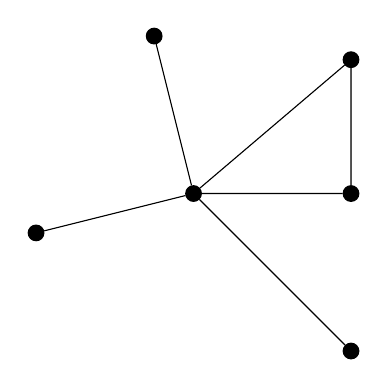
\begin{tikzpicture}
		\node[draw, circle, fill = black, inner sep = 2pt] (A) at (0,0)  {};
		\node[draw, circle, fill = black, inner sep = 2pt] (B) at (2,-2) {};
		\node[draw, circle, fill = black, inner sep = 2pt] (C) at (-2,-0.5) {};
		\node[draw, circle, fill = black, inner sep = 2pt] (D) at (-0.5,2) {};
		\node[draw, circle, fill = black, inner sep = 2pt] (E) at (2,1.7) {};
		\node[draw, circle, fill = black, inner sep = 2pt] (F) at (2,0) {};
		
		\path[draw, fill, black] 
			(A) -- (B)
	 		(A)	-- (C)
   			(A) -- (D)
			(A) -- (E)
			(A) -- (F)
			(E) -- (F);
	\end{tikzpicture}
	
	
	$ S = \{1,...,n\} $ (lo spazio degli stati sono i vertici del grafo)
	
	$ \forall i,j $ abbiamo una costante positiva $ v_{i,j} = v_{j,i} > 0 $.
	
	$ \{i,j\} $ è un arco del grafo.
\end{multicols}

Definiamo la catena di Markov in questo modo:
$$ p_{i,j} = \ddfrac{v_{i,j}}{\sum_{j'}v_{i,j'}} $$

Ci sono degli archi che attirano più di altri il passaggio. Cerchiamo una distribuzione invariante in modo che la catena di Markov sia reversibile:
\begin{align*}
	\alpha_{i}p_{i,j} & = \alpha_{j}p_{j,i} \\
	\alpha_{i}\ddfrac{v_{i,j}}{\sum_{j'}v_{i,j'}} & = 	\alpha_{j}\ddfrac{v_{j,i}}{\sum_{i'}v_{j,i'}} \\
	\ddfrac{a_j}{a_i} & = \frac{\sum_{i'}v_{j,i'}}{\sum_{j'}v_{i,j}}
\end{align*}

Devo scegliere $ k $ in modo che la somma faccia 1:
\begin{align*}
	\sum_{i}\alpha_{i} & = k\sum_{i}\sum_{j'}v_{i,j'} = 1 \\
	k & = \ddfrac{1}{\sum_{i}\sum_{j'}v_{i,j'}}
\end{align*}

In questo modo ho trovato la distribuzione invariante e ho dimostrato che è una catena di Markov reversibile. Se non riesco a risolvere l'equazione non è detto che non ci sia la distribuzione inversa, ma la catena di Markov non è reversibile. 

\section{Metodo Montecarlo basato sulle catene di Markov (MCMC)}
Il metodo Montecarlo è un metodo numerico usato per approssimare usando generatori di numeri casuali. Vediamo un esempio del metodo standard dove si vuole approssimare $\pi$:
\begin{multicols}{2}
	\begin{tikzpicture}
		\begin{axis}[axis lines = center, xtick={-1, 1}, ytick={-1, 1}, ymin = -1.5, ymax=1.5, xmax=1.5, xmin =-1.5, width=7cm, height=7cm]
		
			\draw[thin] (axis cs:0,0) circle [black, radius=1.8cm] ;	
			\draw[thin, black] (axis cs:1,1) -- (axis cs:1,-1) -- (axis cs:-1,-1) -- (axis cs:-1,1) -- (axis cs:1,1);

		\end{axis}
	\end{tikzpicture}
	
	L'area del cerchio è data da:
	$$ A = r^2\cdot \pi = \pi $$
	L'area del quadrato è data da:
	$$ B = (2r)^2 = 4 $$
	$$ \ddfrac{A}{B} = \frac{\pi}{4}$$
	
\end{multicols}

Se scegliamo un punto a caso la probabilità che cada dentro al cerchio è $\frac{\pi}{4}$. Consideriamo una serie di eventi $ E_1, E_2, ... $ (punti scelti a caso nel quadrato):
$$ E_i = (p_i \text{ appartiene al cerchio})$$

Per la legge dei grandi numeri
$$ \ddfrac{\sum_{i=1}^{N} E_i}{N} \simeq \ddfrac{\pi}{4} $$
Per $ N $ molto grande. 

Nel metodo Montecarlo basato su catene di Markov non abbiamo una successione indipendente, ma appunto una catena di Markov. 

Vediamo ora il metodo Montecarlo basato su catene di Markov. Supponiamo di avere un insieme $ S $ finito e una misura di probabilità 
$$ u_s = k\pi_s $$

$ k $ è la costante di normalizzazione. Se $ S $ è molto grande, calcolare $ k $ può essere quasi impossibile. Vogliamo approssimarlo in modo numerico. Per farlo, possiamo generare una catena di Markov ergodica reversibile con $ u_s $ come distribuzione invariante. 

Partiamo da una catena di Markov su $ S $ con probabilità di transizione $ q_{s,s'} $ irriducibile e tale che se $ q_{s,s'} > 0 $ anche $ q_{s',s} > 0 $:

\begin{align*}
	 p_{s,s'} & = \alpha_{s,s'}q_{s,s'} \qquad \text{ per } s' \ne s \qquad 0 \le \alpha_{s,s'} \le 1 \\
	 p_{s,s} & = q_{s,s} + \sum_{s'}(1 - \alpha_{s,s'})q_{s,s'} \\
	 \sum_{s'}p_{s,s'} & = 1
\end{align*}

Ora voglio scegliere $ s' $ in modo tale che la catena abbia come distribuzione invariante $ u_s $:
\begin{align*}
	u_s p_{s,s'} & = u_{s'}p_{s',s} \qquad s' \ne s \; \; \text{\tiny altrimenti la condizione è banalmente verificata} \\
	\pi_s p_{s,s'} & = \pi_{s'}p_{s',s} \qquad \qquad u_s = k\pi_s \\
	\pi_s \alpha_{s,s'}q_{s,s'} & = \pi_{s'}\alpha_{s',s}q_{s',s} \\		
	\ddfrac{\alpha_{s,s'}}{\alpha_{s',s}} & = \ddfrac{\pi_{s'}q_{s',s}}{\pi_s q_{s,s'}} \qquad \qquad \alpha_{s,s'} \le 1 , \; \;  \alpha_{s',s} \le 1
\end{align*}

Definiamo

\begin{align*}
	\alpha_{s,s'} & = \phi \left(\ddfrac{\pi_{s'} q_{s',s}}{\pi_s q_{s,s'}}\right) \\
	\alpha_{s',s} & = \phi \left(\ddfrac{\pi_{s} q_{s,s'}}{\pi_{s'} q_{s',s}}\right) 
\end{align*}

Che proprietà deve avere questa funzione?

\begin{enumerate}
	\item $ 0 \le \phi(x) \le 1 $
	\item $ \ddfrac{\phi(x)}{\phi\left(\frac{1}{x}\right)} = x $
\end{enumerate}

Se io prendo una certa funzione che ha queste proprietà e definisco delle quantità $ \alpha_{s,s'}, \alpha_{s',s} $ sulla quale la funzione è calcolata, allora la proprietà è soddisfatta. %TODO ho riascoltato ma non ho capito benissimissimo 
% quindi per definire una catena di Markov posso  ???

Esistono infinite scelte, ma una possibile scelta per $\phi$ è:
$$ \phi(x) = \min(1,x) $$
Supponiamo $ 0 < x \le 1 $; allora $ \phi(x) = x $ e $ \phi(\frac{1}{x}) = 1 $.

Se invece $ x > 1 $: 
\begin{align*}
	\phi(x) & = 1 \\
	\phi(\frac{1}{x}) & = \frac{1}{x} \\
	\frac{1}{\frac{1}{x}} & = 1
\end{align*}

Definiamo

$$ \alpha_{s,s'} = \min\left(\ddfrac{\pi_s q_{s,s'}}{\pi_{s'}q_{s,s'}}, 1\right)$$

\paragraph{Nota} Abbiamo definito $\phi$ in un certo modo, ma non è l'unico: un'altra possibile funzione è $ \phi(x) = \ddfrac{x}{1+x} $.

Vediamo ora un esempio di applicazione di questo metodo. 

\subsection{Algoritmo di Metropolis-Hastings}
\paragraph{Modello di Ising}
È usato per la meccanica statica, ma può essere applicato al riconoscimento delle immagini. 
$$ S = \{-1, 1\}^\Lambda \qquad \qquad \qquad \Lambda \subset \mathbb{Z}^2 $$

Ho un sottoinsieme di $ \mathbb{Z}^2 $ che posso vedere come un quadrato:

\begin{multicols}{2}
	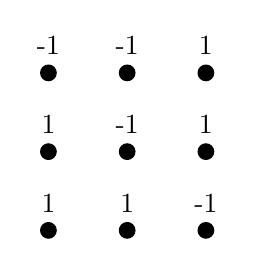
\begin{tikzpicture}
		\node[draw, circle, inner sep=2pt, label=1, fill=black] () at (0,0) {};
		\node[draw, circle, inner sep=2pt, label=1, fill=black] () at (0,1) {};
		\node[draw, circle, inner sep=2pt, label=-1, fill=black] () at (0,2) {};
		\node[draw, circle, inner sep=2pt, label=1, fill=black] () at (1,0) {};
		\node[draw, circle, inner sep=2pt, label=-1, fill=black] () at (1,1) {};
		\node[draw, circle, inner sep=2pt, label=-1, fill=black] () at (1,2) {};
		\node[draw, circle, inner sep=2pt, label=-1, fill=black] () at (2,0) {};
		\node[draw, circle, inner sep=2pt, label=1, fill=black] () at (2,1) {};
		\node[draw, circle, inner sep=2pt, label=1, fill=black] () at (2,2) {};
	\end{tikzpicture}
	\\
	\\
	Se per ognuno di questi punti assegno una quantità, ottengo una configurazione. 
	
	Definisco una misura:
	$$ u_s = k \exp \left[-j \sum_{<i,j>}s_i s_j\right] \qquad \qquad i \in \Lambda $$
\end{multicols}

$ <i,j>: \; i,j $ sono vicini, considero solo coppie di $ i,j $ vicini. 

Per calcolare $ k $ (la costante di normalizzazione) devo fare la somma di tutti i possibili $ s $, che sono: $ |s| = 2^{|\Lambda|} $

Se prendo un quadrato di lato 10, il numero di possibili configurazioni è $ 2^{100} $.

Quindi il problema risiede nel fatto che anche conoscendo il valore della probabilità, è difficile calcolare la costante di normalizzazione; in realtà abbiamo visto nel metodo Montecarlo con le catene di Markov è che la costante non ci serve.

Che funzione posso prendere per $ q_{s,s'} $? Una scelta potrebbe essere scegliere a caso un punto; se è uguale a 1, lo faccio diventare -1 e viceversa. 

Questa $ q $ verifica le proprietà che voglio: se la probabilità di andare da una configurazione all'altra è positiva, ovvero la configurazione si ottiene cambiando in un punto il valore da 1 a -1 o viceversa, è chiaro che anche quella in senso opposto è positiva: se da $ s $ potevo andare in $ s' $, da $ s' $ potevo andare a $ s $. Inoltre questa catena di Markov è irriducibile: se cambio uno alla volta i valori della configurazione posso passare da una configurazione all'altra.

\begin{align*}
	\pi_s & = \exp (j \sum_{<i,j>} s_i s_j) \\
	\alpha_{s,s'} & = \min \left( \frac{\pi_s q_{s,s'}}{\pi_{s'} q_{s',s}} , 1 \right) \\
\end{align*}

$\alpha_{s,s'}$ è diverso da 0 solo se $ q_{s,s'} > 0 $.%, cioè solo se $ s,s' $ sono definiti cambiando di 1. 

$$ \frac{\pi}{\pi_{s'}} = \frac{u_s}{u_{s'}} = \frac{\exp \left[ -j \sum_{<i,j>} s_i s_j
	 \right]}{ \exp \left[ -j \sum_{<i,j>} s_i' s_j' \right] } $$

So che $ s,s' $ sono uguali tranne in un punto. Quindi, tranne che per quel punto, tutte le coppie si cancellano. 

I vicini di un punto in 2 dimensioni sono 4, quindi rimane una somma di 4 termini.

Supponiamo ora di voler calcolare rispetto alla distribuzione invariante qual è la probabilità che un certo punto sia uguale a 1. Bisogna fare la somma delle probabilità di tutte le configurazioni tali che nel punto che sto considerando siano uguali a 1. Come posso approssimarlo usando il metodo Montecarlo? Faccio evolvere le configurazioni nella catena di Markov nel tempo e conto, come nel caso del cerchio, quante volte $ s_p = 1 $ (il mio punto valga 1). Quindi se faccio il rapporto tra quante volte il punto è stato uguale a 1 e il numero di volte che la catena di Markov è evoluta, questo rapporto tende con grande probabilità, per il tempo che tende all'infinito, al valore della probabilità che il punto sia uguale a 1. 

%TODO all'inizio del 28/10/2020 fa un recap dell'algoritmo di metropolis, non so se serva modificare/aggiungere qualcosa detto precedentemente

%Recap: 
L'algoritmo che abbiamo visto si chiama alg. di Metropolis-Hastings ed è appunto basato sul metodo di Monte Carlo basati sulle catene di Markov
Abbiamo visto anche il modello di Ising, dove possiamo applicare appunto l'algoritmo sopra citato. %(https://en.wikipedia.org/wiki/Ising_model#Metropolis_algorithm)
%LEZIONE 28/10/2020 2020-10-28

\subsection{Campionatore di Gibbs (Gibbs sampler)}
È un altro algoritmo basato sulle catene di Markov Monte Carlo. È una versione dell'algoritmo di Metropolis-Hastings. Supponiamo che l'insieme degli stati sia un prodotto cartesiano di $ n $ spazi: 
$$ S = X_1 \times ... \times X_n $$
$$ \underline{s} \in S \qquad \qquad \underline{s} = (x_1, ..., x_n) $$

Gibbs sampler è un caso particolare dell'algoritmo di Metropolis-Hastings; anche qui scegliamo a caso uno dei punti da 1 a $ n $ e ne cambiamo il valore; scegliamo un punto a caso: 
$ \underline{s} $; lo possiamo scrivere come una coppia $ \underline{s} = (\underbrace{s}_1, s_2) $, dove $ \underline{s}_1 $ è la configurazione in tutti gli altri punti, $ s_2 $ è la configurazione in quel punto. %TODO non ho capito esattamente cosa voglia dire

Da questa configurazione possiamo passare ad un'altra configurazione $ \underline{s}' = (\underline{s}_1, s_2') $ che è uguale in tutti gli altri punti, ma differisce solo nel punto scelto sopra. 

Qual è la probabilità di passare da $ s $ a $ s' $?
$$ q_{\underline{s}, \underline{s}'} = \frac{1}{n} P( s_2' | \underline{s}_1 )$$

Quindi vogliamo ottenere una catena di Markov che ha come distribuzione invariante $ k \pi(s) $. Partiamo dalla catena di Markov di riferimento che ha come probabilità di transizione $ q_{\underline{s}, \underline{s}'} $. Quando andiamo a fare il calcolo di $ \alpha_{s,s'} $:

$$ \alpha_{s,s'} = \min\left( \frac{\pi(\underline{s}' q_{\underline{s}', \underline{s}})}{\pi(\underline{s}) q_{s,s'}} , 1   \right) $$ 

osserviamo che 
$$ k\pi(s') q_{\underline{s}', \underline{s}} = k\pi(\underline{s}) q_{\underline{s}, \underline{s}'} $$

Questo perché

$$ k\pi(s) = k\pi(\underline{s}_1)P(s_2, \underline{s}_1) $$ 

e quindi 

$$ \alpha_{s,s'} = \min \left(\frac{\pi(s_1)P(s_2' | \underline{s}_1)}{\pi(s_1)P(s_2 | \underline{s}_1)}, 1\right) $$

$ q_{\underline{s}', s} $ a meno di un fattore è data da $ P(s_2 | \underline{s}_1) $ (e allo stesso modo, nel denominatore al posto di $ q_{s,s'} $ posso scrivere $ P(s_2' | \underline{s}_1) $); quindi $\alpha_{\underline{s},\underline{s'}} = 1$. %TODO ricontrolla apici/pedici

??? %TODO

\chapter{Catene di Markov con tempo continuo}

\section{Distribuzione esponenziale}

Nelle catene di Markov con tempo continuo assume importanza la \textbf{distribuzione esponenziale}. 

Questa distribuzione ha un parametro $\lambda > 0, \lambda \in \mathbb{R}$. 

Consideriamo una variabile aleatoria $ X $ con distribuzione esponenziale di parametro $\lambda$. La funzione di ripartizione ci dà la probabilità che $ X < x $:

$$ F_\lambda (X) = P(X < x) = 
\begin{cases}
	1 - e^{ - \lambda x} & \text{ se } x \ge 0 \\
	0 & \text{ se } x < 0
\end{cases} $$

La distribuzione esponenziale è continua. Dal punto di vista probabilistico, vuol dire che la probabilità che $ X $ sia esattamente uguale a un certo valore è 0. Se la funzione fosse continua, la probabilità sarebbe il salto che fa da un punto ??? %TODO

Introduciamo ora la \textbf{densità di probabilità} $ f_\lambda $:

\begin{align*}
	F_\lambda (x) & = \int_{-\infty}^{x} f_\lambda(y)dy \\
	f_\lambda (x) & = \begin{cases}
		\lambda e ^{-\lambda x} & \text{ se } x \ge 0 \\
		0 & \text{ se } x < 0
	\end{cases}
\end{align*}

La densità non è univocamente definita, potremmo cambiare un punto della funzione e l'integrale non cambierebbe. 

Se abbiamo una variabile aleatoria, possiamo calcolare l'attesa e la varianza. 

Supponiamo di avere $ X $ con distribuzione esponenziale di parametro $\lambda$. L'attesa è data da 

\begin{align*}
	P(X) & = \int_{-\infty}^{+\infty} x f_x(x) dx \\
	& = \int_{0}^{+\infty}x \lambda e ^{-\lambda x}dx \\
	& = \bigg[-xe^{-\lambda x} \bigg]_0^{+\infty} + \int_{0}^{+\infty} e ^{-\lambda x}dx  \\
	& = 0 + \frac{1}{\lambda}\int_{0}^{+\infty} \lambda e^{-\lambda x} dx \\
	& = \frac{1}{\lambda}\bigg[-e^{-\lambda x} \bigg]_0^{+\infty} \\
	& = \frac{1}{\lambda}
\end{align*}

La varianza è:
\begin{align*}
	\text{var}(X) & = P(X^2) - P(X)^2 \\
	\\
	P(X^2) & = \int_{-\infty}^{+\infty} x^2 f_\lambda(x) dx \\
	& = \int_{0}^{+\infty} x^2 \lambda e^{-\lambda x} dx \\
	& = \bigg[-x^2e^{-\lambda x} \bigg]_0^{+\infty} + 2\int_0^{+\infty} x e^{-\lambda x} dx \\
	& = 0 + \frac{2}{\lambda^2} \\
	\\
	\Rightarrow \text{var}(X) & = \frac{2}{\lambda^2} - \frac{1}{\lambda^2} = \frac{1}{\lambda^2}
\end{align*}

Lo \textbf{scarto quadratico medio} è $\sigma(X) = \sqrt{\text{var}(X)} = \ddfrac{1}{\lambda}$. %TODO controlla anche sopra che le X siano X e non x
Questa quantità è la grandezza con cui $ X $ si allontana dalla sua attesa. 

\subsection{Assenza di memoria}

La variabile aleatoria esprime un tempo aleatorio. In questo caso la distribuzione ha una proprietà detta \textbf{assenza di memoria}, collegata alla proprietà di Markov. 

Supponiamo di avere $ X $ con distribuzione esponenziale di parametro $\lambda$. Supponiamo $ x > 0, y > 0 $.

$$ P(X > x + y | X > x) $$

L'interpretazione della probabilità appena enunciata è la seguente: sapendo che $ X > x $, ovvero: sapendo che al tempo $ x $ il fatto $ X $ non si è ancora verificato, ci chiediamo quale sia la probabilità che non si verifichi al tempo $ x+y $:

$$ P(X > x + y | X > x) = \frac{P(X>x+y)}{P(X > x)}$$

perché dobbiamo fare l'intersezione di due eventi, ma $ P(X>x+y) < P(X>x) $

\begin{align*}
	& = \frac{1 - F_\lambda (x+y)}{1-F_\lambda(x)} \\
	& = \frac{1- (1-e^{-\lambda(x+y)})}{1-(1-e^{\lambda x})} \\
	& = \frac{e^{-\lambda(x+y)}}{e^{-\lambda x}} \\
	& = e^{-\lambda y} \\
	& = P(X > y)
\end{align*}

Interpretazione: se al tempo $ x $ non si è ancora verificato l'evento, qual è la probabilità che si verifichi dopo un ulteriore tempo $ y $? È la stessa cosa che chiedersi direttamente se l'evento si verifica dopo il tempo $ y $, come se ripartisse dall'inizio. 
\\
\\
\\
Vediamo altre proprietà. Supponiamo di avere due tempi indipendenti $ X, Y $ con distribuzioni esponenziali di parametri rispettivamente $\lambda_1, \lambda_2$. Consideriamo
$$ Z = \min(X, Y) $$.

Qual è la distribuzione di $ Z $? $ Z $ avrà ancora distribuzione esponenziale di parametro $ \lambda_1 + \lambda_2 $. Consideriamo un $ x > 0 $. Calcoliamo

\begin{align*}
	P(Z < x) & = 1 - P( > Z) \\
	& = 1 - P(\min(X, Y) > x) \\
	& = 1 - P((X > x)(Y > x)) \\
	& = 1 - P(e^{-\lambda_1 x} e^{-\lambda_2 x}) \\
	& = 1 - e^{-(\lambda_1 + \lambda_2)x}
\end{align*}

Chiediamoci ora $ P(X < Y) $ (nota: possiamo chiederci anche $ P(X > Y) $, ma $ P(X=Y) $ è 0 perché essendo la distribuzione continua la probabilità che assuma un certo valore è 0):

\begin{align*}
	& = \int_{0}^{+\infty} (1- e^{-\lambda_1 y}) \lambda_2 e^{-\lambda_2}y dy \\
	& = \int_{0}^{+\infty} \lambda_2 e^{-\lambda_1 y} dy -\lambda_2 \int_{0}^{+\infty} e^{-(\lambda_1 + \lambda_2)y} dy \\
	& = 1 - \frac{\lambda_2}{\lambda_1 + \lambda_2} \\
	& = \frac{\lambda_1}{\lambda_1 + \lambda_2}
	& \Rightarrow P(Y < X) = \frac{\lambda_1}{\lambda_1 + \lambda_2}
	\\
	\\
	& P(Y < X) + P(X < Y) = 1 %TODO controlla che Y < X non sia Y < x e viceversa
\end{align*}

Possiamo estenderlo al caso di $ n $ variabili aleatorie indipendenti $ X_1, X_2, ..., X_n $ di parametri $ \lambda_1, \lambda_2, ..., \lambda_n $:

$$ Z = \min(X_1 + ... + X_n) $$

Possiamo fare il minimo tra $ X_1 $ e $ X_2 $, poi il minimo con $ X_3 $ etc. 
$ Z $ ha una distribuzione esponenziale di parametro $ \lambda_1 + \lambda_2 + ... + \lambda_n $ e 
\begin{align*}
	P(Z = X_i) & = P(X_i < \min(X_1, ..., X_{i-1}, X_{i+1}, ..., X_n)) \\
	& = \frac{\lambda_i}{\lambda_1 + \lambda_2 + ... + \lambda_n}
\end{align*}

\subsection{Tasso di rischio} %TODO è una sottosezione?
Quando abbiamo una variabile aleatoria con una distribuzione esponenziale si considera una funzione detta \textbf{tasso di rischio}. %TODO negli appunti c'è scritto turard rate che non esiste

Sia $ X $ una variabile aleatoria con densità $ f(x), \; x > 0 $ e $ f(x) = 0 $ per $ x < 0 $.

Consideriamo $ P(t \le X \le t+1 | X > t) $; il tasso di rischio $ r(t) $ è:

$$ r(t) = \lim\limits_{\Delta \to 0} \frac{P(t \le X \le t+1 | X > t)}{\Delta}$$ %TODO che cacchio è delta

Che relazione c'è tra la densità di probabilità e il tasso di rischio?

$$ r(t) = \lim\limits_{\Delta \to 0} \frac{\int_{t}^{t + \Delta} f(x)dx }{(1 - F(t))\Delta}$$ 

Siccome $\Delta$ tende a 0, l'integrale è calcolato nel punto $ t $:

$$ = \frac{f(t)}{1 - F(t)} $$

Osservazione:
\begin{align*}
	r(t) & = -\frac{\partial}{\partial t} \log (1 - F(t)) \\
	& = - \frac{-f(t)}{1 - F(t)} \\
	& = \frac{f(t)}{1 - F(t)}
\end{align*}

Siccome $ F(0) = 0 $ e $ \log(1 - F(0)) = 0 $ possiamo scrivere che 
\begin{align*}
	\log(1 - F(t)) & = -\int_{0}^{t} r(s) ds \\
	1 - F(t) & = \exp \left( - \int_{0}^{t} r(s)ds \right) \\
	F(t) & = 1 - \exp \left( - \int_{0}^{t} r(s)ds \right)
\end{align*}

Questa è la formula che ci permette di calcolare la funzione di ripartizione per una variabile aleatoria sapendo il tasso di rischio. Se il tasso di rischio è pari a $\lambda$:
$$ r(s) = \lambda \qquad \qquad \qquad F(t) = 1 - e^{-\lambda t}$$ 

\subsection{Distribuzione iperesponenziale}

Partendo dalla distribuzione esponenziale possiamo ottenere un'altra distribuzione che si ottiene facendo una somma di tante distribuzioni esponenziali: supponiamo di avere $ X_1, X_2, ..., X_n $ variabili aleatorie indipendenti con distribuzione esponenziale di parametri $ \lambda_1, ..., \lambda_n $ rispettivamente. 

Supponiamo di avere una variabile aleatoria $ X $ indipendente da $ X_1, ..., X_n $.

$$ P(X = j) = p_j \qquad \qquad j = 1, ..., n $$

$ X_T $ è iperesponenziale.

\begin{align*}
	P(X_T > t) & ??? \\ %TODO
	\\
	P(X_T) & = \sum_{j=1}^{n} P(X_T > t | t = j) P (T = j) \\
	& = \sum_{j = 1}^{n} e ^{-\lambda_j t} p_j
\end{align*}

Questa non ha la proprietà di assenza di memoria e non è una distribuzione esponenziale. 


%TODO 3/11/2020 hai perso l'inizio

Qual è il tasso di rischio di questa? %TODO esprimiti in modo meno rozzo

$$ r(t) = \frac{\sum_{i = 1}^{n} p_i \lambda_i e^{-\lambda_i t}}{\sum_{i = 1}^{n} p_i e^{-\lambda_i t}} $$

Il tasso di rischio non è costante. Vogliamo vedere cosa succede al limite. 

Supponiamo che $\lambda_1$ sia il minimo dei $\lambda_i, \lambda_i = \lambda_1 + ... + i + 1$ %TODO controlla sia corretto

$$ r(t) = \sum_{i = 1}^{n} p_i(\lambda_i e ^{(-\lambda_i - \lambda_1) t } \underset{t \to \infty}{\longrightarrow} \lambda_1) $$
$$ ??? $$ %TODO controlla anche sopra

La distribuzione esponenziale decade più lentamente delle altre. ??? %TODO

Comunque non è costante, dipende dal tempo. 

Vediamo qual è la somma di due variabili indipendenti con distribuzione esponenziale. Presentiamo prima un esempio nel caso discreto. Supponiamo di avere due variabili $ X, Y $ indipendenti con distribuzione di Poisson di parametri rispettivamente $\lambda_1, \lambda_2$. Sia $ Z = X + Y $. Qual è la distribuzione di $ Z $? Dobbiamo vedere qual è la probabilità che $ Z $ sia uguale ad un certo valore. 
\begin{align*}
	P(Z = u) & = \sum_{k = 0}^{n} P(X = k)P(Y = n-k) & n \ge 0 \\
	& = \sum_{k=0}^{n} \frac{\lambda_1^k e^{-\lambda_1}} {k!} \frac{\lambda_2^{n-k} e^{-\lambda_2}}{(n-k)!} \\
	& = \frac{e^{-(\lambda_1 + \lambda_2)}}{n!} \sum_{k=0}^{n} \underbrace{\binom{n}{k} \lambda_1^k \lambda_2^{n-k}}_{\text{binomio di Newton}} \\
	& = \frac{(\lambda_1 + \lambda_2)^n}{n!} e^{-(\lambda_1 + \lambda_2)}
\end{align*}

Vediamo ora il caso continuo. $ X $ e $ Y $ sono due variabili aleatorie indipendenti con densità $ f(t), g(t) $ rispettivamente. Vogliamo analizzare $ Z = X + Y$. Sia $ l $ la densità di $ Z $. 

\begin{align*}
	h(t) & = \int f(u) g(t-u) du ??? \\%TODO
	& = f * g(t) \qquad \qquad \text{ convoluzione di } f \text{ e } g
\end{align*}

La \textbf{convoluzione} è un'operazione che si può fare in generale e che date due funzioni ne restituisce una. 

Proprietà della convoluzione: 
\begin{enumerate}
	\item proprietà commutativa: $ f * g = g*f $
	\item bilinearità: $ f * (ag + bh ) = af * g + bf * h $ ??? %TODO
\end{enumerate}

Vogliamo applicare la convoluzione per studiare la somma di due variabili indipendenti con distribuzione esponenziale di parametro $ \lambda $: $ Z = X + Y $. La densità di $ X $ e $ Y $ è $ g_\lambda $. Calcoliamo la densità di $ Z $:
\begin{align*}
	h(t) & = g_\lambda * q_\lambda(t) \\
	& = \int g_\lambda(u) g_\lambda(t-u) du
\end{align*}

La densità esponenziale è positiva se ??? %TODO
è positiva, quindi se $ u $ è negativa è 0 e se $ t-u $ è negativa è 0: %TODO eh????

\begin{align*}
	& = \int_{0}^{t} \lambda e ^{-\lambda u} \lambda e^{-\lambda(t-u)} du \\
	& = \lambda^2 e^{-\lambda t} \int_{0}^{t} du \\
	& = \lambda^2 t e^{-\lambda t} & t \ge 0
\end{align*}

\subsection{Distribuzione di Erlanger} %TODO è scritto bene? possiamo considerarlo una sottosezione?
In generale cosa succede se facciamo la somma di $ n $ variabili aleatorie $ X_1, ..., X_n $ indipendenti, con distribuzioni esponenziali di parametro $\lambda$? 

Supponiamo $ Z = X_1 + ... + X_n $; $ Z $ ha densità $ h(t) $ con $ t > 0 $:

$$ h(t) = \frac{\lambda^n t^{n-1}}{(n-1)!} e^{-\lambda t} $$

Questa è chiamata distribuzione di Erlang di parametri $ (\lambda, n) $.

È possibile dimostrare l'uguaglianza soprastante per induzione. 

Supponiamo sia vera fino a $ n-1 $. Sappiamo che $ Z = X_1 + ... + X_n $; possiamo riscriverla come 
$ Z = (X_1 + ... + X_{n-1}) + X_n $

Siccome $ X_1, ..., X_n $ sono indipendenti, anche la somma evidenziata dalle parentesi tonde è indipendente da $ n $ e possiamo usare la convoluzione:

\begin{align*}
	h(t) & = \int_{0}^{t}\frac{\lambda^{n-1} u^{n-2}}{(n-2)!} e^{-\lambda u} \lambda e^{-\lambda(t-u)} du \\
	& = \frac{\lambda^n}{(n-2)!}e^{-\lambda t} \int_{0}^{t} u^{n-2} du \\
	& = \frac{\lambda^n}{(n-2)!} e^{-\lambda t} \frac{t^{n-1}}{n-1} \\
	& = \frac{\lambda^n t^{n-1}}{(n-1)!} e^{-\lambda t} ??? %TODO controlla da (n-1)!
\end{align*}

La distribuzione di Erlang, a differenza della distribuzione esponenziale, non ha la proprietà di assenza di memoria. Però posso rappresentarla come una somma di variabili aleatorie indipendenti. 

Vediamo ora il caso di $ n $ variabili aleatorie con parametri $ \lambda_1, ..., \lambda_n $ tutti diversi tra loro. Iniziamo studiando la somma tra due variabili $ X $ e $ Y $.

Sia $ Z = X + Y $ e $ h(t) $ la densità di $ Z $:
\begin{align*}
	h(t) & = \int g_{\lambda_1}(u) g_{\lambda_2}(t-u) du \\ %TODO i \lambda sono pedici di g?
	& = \int_{0}^{t} \lambda_1e^{-\lambda_1 u} \lambda_2e^{-\lambda_2(t-u)} du \\
	& = \lambda_1\lambda_2e^{-\lambda_2 t} \int_{0}^{t}e^{-u(\lambda_1-\lambda_2)} du \\
	& = \lambda_1\lambda_2e^{-\lambda_2 t} \bigg[\frac{e^{-u(\lambda_1-\lambda_2)}}{\lambda_2 - 
		\lambda_1}\bigg]^{t}_0 \\
	& = \frac{\lambda_1\lambda_2 e^{-\lambda_2 t}}{\lambda_2 - \lambda_1}e^{-(\lambda_1 - \lambda_2)t} + \frac{\lambda_1\lambda_2}{\lambda_1-\lambda_2}e^{-\lambda_2 t} \\
	& = \frac{\lambda_2}{\lambda_2 - \lambda_1} \lambda_1 e^{-\lambda_1 t} + \frac{\lambda_1}{\lambda_1 - \lambda_2}\lambda_2 e^{-\lambda_2t} \\
	\Rightarrow g_{\lambda_1} * g_{\lambda_2} & = \frac{\lambda_2}{\lambda_2 - \lambda_1} g_{\lambda_1} + \frac{\lambda_1}{\lambda_1-\lambda_2}g_{\lambda_2} %TODO i \lambda sono pedici di g?
\end{align*}

Consideriamo ora effettivamente $ n $ distribuzioni esponenziali $ X_1, X_2, ..., X_n $ indipendenti con parametri $ \lambda_1, ..., \lambda_n $ diversi tra loro. Bisogna fare una convoluzione di $ n $ parametri, nell'ordine che si preferisce. 

??? %TODO

Mi basta il coefficiente. 

$$ \begin{array}{ccc} %TODO controlla che i lamba siano effettivamente apici
 \text{ Convoluzione con } & g_{\lambda_1}: & \frac{\lambda_1}{\lambda_1 - \lambda_i} \\
 & g_{\lambda_2} : & \frac{\lambda_2}{\lambda_2  - \lambda_1} \\
 & ... & \\
 & g_{\lambda_n}: & \frac{\lambda_n}{\lambda_n - \lambda_i}
\end{array}$$

%TODO ora sugli appuniti c'è la roba che ho appena scritto ma in orizzontale, è importante ricopiarla?

La densità di $ X_1 + ... + X_n $ è:
$$ h(t) = \sum_{i = 1}^n \prod_{j \ne i}^{n} \frac{\lambda_j}{\lambda_j - \lambda_i} g_{\lambda_i}$$
Sembra analoga alla distribuzione iperesponenziale, ma non è così perché i coefficienti non sono necessariamente tutti positivi. Infatti il denominatore ha la differenza $ \lambda_j - \lambda_i $, quindi può assumere valori negativi. Questa distribuzione si chiama \textbf{ipoesponenziale.} %TODO la mettiamo in una sezione?

Il fattore di rischio non è costante. Cosa succede mandando il tempo all'infinito? Supponiamo $\lambda_1$ sia il più piccolo di tutti: $\lambda_1 = \min(\lambda_1, ..., \lambda_n)$

$$ \prod_{i \ne 1, j\ne 1}^{n} \left(\frac{\lambda_j}{\lambda_j - \lambda_i}\right) g_{\lambda_1} ??? $$ %TODO

Tasso di rischio:
$$ r(t) \frac{\sum_{i=1}^{n}\prod_{j\ne i}^{n} \left(\frac{\lambda_j}{\lambda_j - \lambda_i}\right)g_{\lambda_i}}{\sum_{i=1}^{n}\prod_{j\ne i}^{n} \left(\frac{\lambda_j}{\lambda_j - \lambda_i}\right) e^{-\lambda_i t}} ??? $$%TODO

\begin{align*}
	\lambda_1 & = \min(\lambda_1, ..., \lambda_n) \\
	& r(t) \underset{t \to \infty}{\longrightarrow} \lambda_1
\end{align*}

\chapter{Processo di Poisson}
Fa parte di una famiglia di processi detti processi di conteggio, un tipo di processo che descrive il numero di volte in cui si verifica un certo fatto al variare del tempo: $ N_t, t \ge 0 $ indica quante volte si è verificato un fatto (es. decadimento radioattivo, arrivo di un cliente allo sportello...) dal tempo 0 al tempo $ t $.

\paragraph{Proprietà dei processi di conteggio}
\begin{enumerate}
	\item $ N_0 = 0 $;
	\item $ N_t $ ha valori naturali;
	\item $ N_t $ è non decrescente (quindi può rimanere uguale).
\end{enumerate}

Il processo di Poisson con parametro $\lambda$ è un processo di conteggio $ N_t $ con in più le seguenti proprietà:
\begin{enumerate}
	\item per $ 0 \le t_1 \le t_2 $, $ N_{t_2} - N_{t_1} $ (numero di fatti verificatisi tra $ t_1 $ e $ t_2 $) ha distribuzione di Poisson di parametro $\lambda(t_2 - t_1)$;
	\item ha incrementi indipendenti.
\end{enumerate}

L'ultimo punto vuol dire che se si prendono tanti intervalli disgiunti $ (0, t_1], (t_1, t_2], ..., (t_{n-1}, t_n] $  con $ 0 \le t_1 < t_2 < ... < t_n $, allora $ N_{t_1}, N_{t_2} - N_{t_1}, ..., N_{t_n} - N_{t_{n-1}} $ sono indipendenti.

Osservazione di compatibilità: se prendo $ (0, t_1 ], (t_1, t_2], ..., (0, t_2] $:
$$ N_{t_2} - N_0 = (N_{t_2} - N_{t_1}) + (N_{t_1} - N_0) $$

Queste distribuzioni (di parametri rispettivamente $\lambda(t_2 - 0),\lambda(t_2 - t_1),\lambda(t_1 - 0) $) sono indipendenti. 

Supponiamo di prendere $ u_1, ..., u_n $ indipendenti con distribuzioni esponenziali di parametro $\lambda$. Immaginiamo che $ u_1, ..., u_n $ descrivano il tempo d'arrivo di clienti ad uno sportello. Allora
$$ T_k = u_1 + ... + u_n $$

ovvero $ T_k $ è il tempo dell'arrivo del cliente k-esimo. Posso descrivere un processo di conteggio (quanti clienti sono arrivati entro il tempo $ t $?)

$$ N_t = \max \{k | T_k \le t \}, \qquad \qquad T_k \le t \le T_{k+1} $$

Allora $ N_t $ è un processo di Poisson di parametro $\lambda$.

Quanto vale quindi $ P(N_t = k) $?

\begin{align*}
	P(N_t = k) & = P(T_k \le t < T_{k+1}) \\
	& = P((T_k \le t) \ (T_{k+1} \le t)) \\
	& = P(T_k \le t) - P(T_{k+1} \le t)
\end{align*}
\\
\\
\\
\hrule\vfill
%TODO 2020-11-04 hai perso l'inizio!
Possiamo dire che


$$ P(X_k \le t) - P (X_{k+1} \le t) = \int_{0}^{t} \frac{\lambda^k s^{k-1}}{(k-1)!} e^{-\lambda s} ds - \int_{0}^{t} \frac{\lambda^{k+1} s^{k}}{k!} e^{- \lambda s} ds $$
Integro per parti:
\begin{align*}
	& = \lambda^k \bigg[\frac{s^k}{k!} e^{-\lambda s}\bigg]_0^{t} + \int_{0}^{t} \frac{\lambda^{k+1} s^{k}}{k!} e^{- \lambda} ds - \int_{0}^{t} \frac{\lambda^{k+1} s^{k}}{k!} e^{- \lambda s} ds \\
	& = \frac{\lambda^k t^k}{k!} e^{-\lambda t}
\end{align*}

Ma questa è la probabilità del processo di Poisson ??? %TODO

Adesso devo verificare l'indipendenza: ??? %TODO
intervalli separati sono indipendenti.

\begin{center}
	\begin{tikzpicture}
		\draw (0,0) -- (10,0);
		\draw (4,-0.15) -- (4,0.15);
		\draw (6,-0.15) -- (6,0.15);
		\node[label=below:u] (A) at (4,0) {} ;
		\node[label=below:t] (B) at (6,0) {} ;
	\end{tikzpicture}
\end{center}

Prendiamo l'intervallo tra 0 e $ u $; ci chiediamo quanto vale
$$ P(N_t - N_u = k | N_s, s \le u) $$

??? %TODO

$$ \frac{\lambda(t-u)^k}{k!} e^{-\lambda(t-u)} $$

Questo rapporto tra distribuzione esponenziale e processo di Poisson ci permette di trovare un metodo per simulare il processo di Poisson.

Consideriamo una successione di ??? %TODO

Come si fa a generare una successione di variabili aleatorie con distribuzione esponenziale? Si usa questo fatto: sia $ Z $ una variabile con distribuzione uniforme in $ [0,1] $ e sia $ F $ la funzione di ripartizione dell'esponenziale:
$$ F(x) = \begin{cases}
	1 - e^{-\lambda x} & \text{se } x \ge 0 \\
	0 & \text{se } x < 0
\end{cases} $$

$ F $ è una funzione strettamente crescente. Posso considerare la funzione inversa $ F^{-1} $, e quello che si vede è che $ F^{-1}(Z) = W $ è una variabile aleatoria con distribuzione esponenziale di parametro $\lambda$. 

Esempio:

\begin{align*}
	P(W \le x & = F^{-1})(Z \le x) \\
	& = P(Z \le F(x)) \\
	& = F(x)
\end{align*}

In questo caso è facile anche calcolare l'inversa:
\begin{align*}
	x & = F^{-1}(y) \\
	F(x) & = y \\ %TODO ricontrolla y e Y etc.
	y & = 1 - e^{-\lambda x} \\
	e^-{-\lambda x} & = 1 - y \\
	-\lambda x & = \log(1-y) \\
	x & = - \frac{1}{\lambda} \log (1-y)
\end{align*}

Se prendo una variabile aleatoria $ U $ con distribuzione uniforme su $ [0,1] $ e definisco $ W $:
$$ W = \frac{1}{\lambda} \log(1 - U) $$
$ W $ è una distribuzione esponenziale di parametro $\lambda$.

Abbiamo visto il caso di una sola variabile; se vogliamo generare una successione di variabili $ U_1, U_2, ... $ indipendenti con distribuzioni uniformi in $ [0,1] $ definisco $ W_1, W_2, ... $ nel seguente modo:

$$ W_i = \frac{1}{\lambda} \log(1 - U_i) $$

Osservazione: in base alla definizione di processo di Poisson è un conteggio a valori interi non decrescenti. %TODO che cosa?

In linea di principio un processo di Poisson potrebbe fare salti maggiori di 1, in realtà la probabilità che accada è 0. 

Consideriamo un intervallo $ [0,t] $ e dividiamolo in intervalli di lunghezza $\frac{1}{2^N}$.

Qual è la probabilità che in uno di questi intervalli il processo di Poisson faccia un salto più grande di 1? Siccome ??? %TODO
 questo è uguale alla probabilità che nel primo salto non faccia salti più grandi di 1, elevato al numero degli intervalli:
\begin{align*}
	(P(N_{\frac{1}{2}N} \le 1))^{2^N} & = (P(N_{\frac{1}{2}N} = 0) + P(N_{\frac{1}{2}N} = 1) )^{2^N} \\
	& = ( e^{-\frac{\lambda}{2^N}} + \frac{\lambda}{2^N}e^{-\frac{\lambda}{2^N}}  )^{2^N} \\
	& = e^{-\lambda}(1 + \frac{\lambda}{2^N})^{2^N} \\
	\\
	\lim\limits_{N \to \infty} e^{-\lambda}(1 + \frac{\lambda}{2^N}) & = 1
\end{align*}

??? %TODO
Quindi non ci sono salti più grandi di 1.
??? %TODO
Quindi o non ha salti oppure ha tutti salti di grandezza 1.

\section{Decomposizione di un processo di Poisson}
È un'altra proprietà dei processi di Poisson. Supponiamo di avere un processo di Poisson di parametro $\lambda$ che descrive gli arrivi dei clienti ad un supermercato (quanti clienti sono arrivati prima di un tempo $ t $). Dividiamo i clienti in due categorie, ad esempio maschi e femmine. Il cliente è in una certa categoria, ad esempio "maschi", con probabilità $ p $ ed è nell'altra categoria con probabilità $ 1-p $. È come se ogni volta che arriva un cliente tirassimo una moneta, se esce testa finisce nella prima categoria, se esce croce nella seconda. 

Possiamo allora scrivere il nostro processo come due processi di conteggio:
$$ N_t = N_t^{(1)} + N_t^{(2)} $$

$ N_t^{(1)} $ e $ N_t^{(2)} $ sono due processi di Poisson indipendenti. 

Vogliamo calcolare ora:

\begin{align*}
	P(N_t^{(1)} = k_1, N_t^{(2)} = k_2) & = P(N_t^{(1)} = k_1, N_t^{(2)} = k_2 | N_t = k_1 + k_2) P(N_t = k_1 + k_2) \\
	& = p \binom{k_1 + k_2}{k_1} p^{k_1} (1-p)^{k_2} - \frac{(\lambda t)^{k_1 + k_2}}{(k_1 + k_2)!} e^{-\lambda t} \\
	& = \frac{(\lambda p t)^{k_1}}{k_1!} \frac{\big[ \lambda(1-p)t \big]^{k_2}}{k_2!} e^{-\lambda p t} e^{-\lambda(1-p) t} \\
	& = \frac{(\lambda p t)^{k_1}}{k_1!} e^{-\lambda p t} \frac{\big[ \lambda(1-p) t \big]^{k_2}}{k_2 !} e^{-\lambda (1-p) t}
\end{align*}

$ N_t^{(1)} $ è processo di Poisson di parametro $\lambda p$

$ N_t^{(2)} $ è processo di Poisson di parametro $\lambda(1-p)$

In questo modo abbiamo mostrato per un solo intervallo che sono indipendenti %TODO what
, dobbiamo ancora verificare che gli incrementi su intervalli separati siano indipendenti.

Ma siccome partiamo già da variabili aleatorie indipendenti, otterremo ancora ??? %TODO

Questo si può generalizzare nella decomposizione in $ n $ processi di Poisson: consideriamo

$$ P_1, P_2, ..., P_n \qquad \qquad P_1 + P_2 + ... + P_n  = 1 \qquad 0 \le p_i \le 1 $$
$$ N_t = N_t^{(1)} + ... + N_t^{(n)} $$

I processi $ N_t^{(1)}, ..., N_t^{(n)} $ sono anche loro di Poisson indipendenti di parametri rispettivamente $ \lambda_{p_1}, ..., \lambda_{p_n} $.

Lo stesso argomento si può mostrare al contrario: supponiamo di avere $ N_t^{(1)}, ..., N_t^{(n)} $ processi di Poisson indipendenti di parametri $ \lambda_{1}, ..., \lambda_{n} $. Definiamo:
$$ N_t = N_t^{(1)} + ... + N_t^{(n)} $$

Allora $ N_t $ è è processo di Poisson di parametro $ \lambda = \lambda_{1} + ... + \lambda_{n} $.

Supponiamo $ N_t $ sia un processo di Poisson di parametro $ \lambda = \lambda_{p_1} + ... + \lambda_{p_n} $; definiamo 
$$ p_1  = \frac{\lambda_1}{\lambda_1 + ... + \lambda_{n}}, ... , p_n = \frac{\lambda_{n}}{\lambda_{1} + \lambda_{n}}$$
$ N_t^{(1)}, ..., N_t^{(n)} $ sono indipendenti di parametro $\lambda_{p_i} = \lambda_{i}$

\section{Definizione equivalente di processo di Poisson}
Processo di conteggio con incrementi indipendenti 
$$ P(N_{t + h} = N_t) = 1 - \lambda h t + o(t) $$
$$ P(N_{t + h} = N_t + 1) = \lambda h + o(h) $$
??? uniforme in $ t $ %TODO

Cioè anziché ??? %TODO
$ o(h) $: infinitesimo di ordine superiore ad $ h $, ovvero quantità tale che:
$$ \lim\limits_{h \to 0} \frac{o(h)}{h} = 0 $$

Vogliamo mostrare che le due definizioni sono equivalenti. 

Qual è la probabilità di nessun incremento?
\begin{align*}
	P(N_{t+h} = N_t) & = e^{-\lambda h} \\
	& = 1 - \lambda h + o(h)
\end{align*}

Incremento di 1?
\begin{align*}	
	P(N_{t+h} = N_t + 1) & = \lambda h e^{-\lambda h } \\ 
	& = \lambda h (1 - \lambda h + o(h)) \\
	& = \lambda h - \lambda^2 h^2 + o(h^2) \\
	& = \lambda h + o(h)
\end{align*}

Incremento $ k \ge 2 $?

\begin{align*}	
	P(N_{t+h} = N_t + k) & \le 1 - P(N_{t+h} = N_t) - P(N_{t+h} = N_t + 1) \\
	& = 1 - (1 - \lambda h - o(h)) - \lambda h - o(h) \\
	& = o(h)
\end{align*}

Quindi la probabilità di fare un salto più grande di 2 è un infinitesimo di ordine superiore a $ h $. 

Il processo di Poisson soddisfa queste condizioni. ??? %TODO
Per concludere la dimostrazione che le due definizioni sono equivalenti, dobbiamo mostrare anche l'altro verso dell'implicazione, cioè ??? %TODO

\begin{align*}
	P(N_{t+h} = 0) & = P(N_t = 0) P(N_{t+h} - N_t = 0) \\
	\\
	P(N_{t+h} = 0) - P(N_t = 0) & = P(N_{t+h} - N_t = 0 - 1 )P(N_t = 0) \\
	\\
	u_t & = P(N_t = 0) \\
	\\
	u_{t+h} - u_t & = 0 \\
	& = ((1 - \lambda h + o(h)) - 1 ) u_t \\
	\frac{u_{t+h} - u_t}{h} & = \lambda u_t + \frac{o(h)}{h} \\
	\\
	\lim\limits_{h \to 0} u'_t & = \lambda u_t & u_0 = 1
\end{align*}

$$ 	??? ke^{-\lambda t} \qquad \qquad k = 1$$
$$ u_t = e^{-\lambda t} \qquad \qquad P(N_t = 0) e^{-\lambda t} $$

Questo corrisponde al processo di Poisson. Devo farlo vedere anche per valori diversi.

Consideriamo $ P(N_{t+h} = k), k \ge 1 $
Si può verificare in due modi:
$$ P(N_{t+h} = k) = P(N_t = k) P(N_{t+h} - N_t = 0) $$
Oppure
$$ P(N_{t+h} = k) = P(N_t = k-1)P(N_{t+h} -N_t = 1) + o(h) $$
??? %TODO

$$ P(N_{t+h} = k) - P(N_t = k) = -(\lambda h + o(h)) P(N_{t} = k) + P(t = k - 1)(\lambda h + o(h)) + o(h) $$

Definiamo $ U_k^{(t)} = P(N_{t} = k) $

\begin{align*}
	\frac{u_{t+h}^{(t)}  - u_t^{(k)} }{h} & = -\lambda u_t^{(k)} + \frac{o(h)}{o} + \lambda_{u_t}(k-1) + o(h) \\
	u_t^{(k)} & = -\lambda_{u_t}^{(k)} + \lambda_{u_t}^{(k-1)} & u_t^{(0)} = e^{-\lambda t}
\end{align*}

Verifico ??? %TODO
$$ u_t^{(k)} = \frac{(\lambda t)^k}{k!} e^{-\lambda t} $$

Deriviamo:
$$ u_t'^{(k)}= \frac{\lambda k (\lambda t)^{(k-1)}}{k!} e^{-\lambda t} -\lambda\frac{(\lambda t)^k}{k!} e^{-\lambda t} $$
La soluzione di questa equazione differenziale è quella data dalla soluzione del processo di Poisson. 

%TODO 2020-11-10

\section{Distribuzione condizionata dei punti di salto}
Sia $ T $ il primo punto di salto. Vogliamo calcolare $ P( a < T \le b | N_u = 1) $, con $ 0 \le a < b \le u $. Sapendo che al tempo $ u $ c'è stato un solo salto (il processo di Poisson è uguale a 1), qual è la probabilità che ci sia un salto in $ (a,b] $?

Vogliamo mostrare che $ P( a < T \le b | N_u = 1) = \frac{b-a}{u} $.

Sia $ N_T $ un processo di Poisson con parametro $\lambda$:

\begin{align*}
	P( a < T \le b | N_u = 1) & = \frac{P( a < T \le b | N_u = 1)}{P(N_u = 1)} \\
	& = \frac{P(N_a = 0, N_b - N_a = 1, N_u - N_b = 0)}{P(N_u = 1)} \\
	& = \frac{ \cancel{e^{-\lambda a}} (\bcancel{\lambda} (b-a)) \cancel{e^{-\lambda(b-a)}} \cancel{e^{-\lambda(u-b)}}  }{(\bcancel{\lambda} u) \cancel{e^{-\lambda u}}} \\
	& = \frac{b-a}{u}
\end{align*}

La stessa cosa è dimostrabile nel caso di $ n $ salti. Vediamo per esempio il caso $ n = 2 $. 

Siano $ T_1, T_2 $ i primi due salti. Consideriamo due intervalli $ (a,b] $ e $ (c,d] $ con $ 0 \le a < b < c < d \le u $.

Vogliamo calcolare:

$$ P(a < T_1 \le b, c < T_2 \le d | N_u = 2) $$

Ovvero qual è la probabilità che ci siano due salti:

\begin{align*}
	& = \frac{P(N_a = 0, N_b - N_a = 1, N_c - N_b = 0, N_d - N_c  = 1, N_u - N_d  = 0)}{N_u = 2} \\
	& = \frac{  \cancel{e^{-\lambda a}} (\bcancel{\lambda}(b-a)) \cancel{e^{-\lambda(b-a)}} e^{-\lambda(b-c )}    (\bcancel{\lambda}(d-c)) \cancel{e^{-\lambda(d-c)}} \cancel {e^{-\lambda(u-d)}}  } {\frac{(\bcancel{\lambda }u)^2}{2} \cancel{e^{-\lambda u}}} \\ %TODO qualcosa non torna con la roba che si semplifica
	& = 2 \frac{(b-a)(d-c)}{u^2}
\end{align*}

Possiamo visualizzare $ T_1 $ e $ T_2 $ come punti del piano:
\begin{center}
	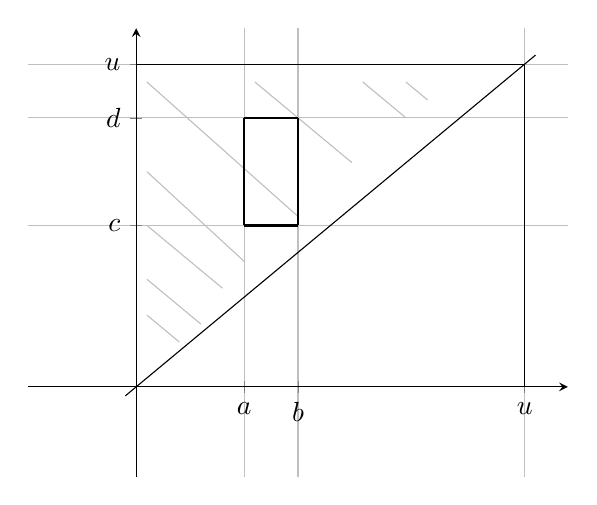
\begin{tikzpicture}
		\begin{axis}[axis lines = middle, grid, xtick={1,1.5,3.6}, xticklabels={$ a $,$ b $, $ u $}, ytick={1.8,3,3.6}, yticklabels={$ c $, $ d $, $ u $}, xmin = -1, ymin = -1, xmax = 4, ymax = 4]
		
		\draw[black] (axis cs: 3.6,0) --(axis cs: 3.6,3.6);
		\draw[black] (axis cs: 0,3.6) --(axis cs: 3.6,3.6);
		
		\addplot[black, tiny, domain=-0.1:3.7] {x+0};
		\draw[lightgray] (axis cs:0.4,0.5) -- (axis cs:0.1, 0.8);
		\draw[lightgray] (axis cs:0.6,0.7) -- (axis cs:0.1, 1.2);
		\draw[lightgray] (axis cs:0.8,1.1) -- (axis cs:0.1, 1.8);
		\draw[lightgray] (axis cs:1,1.4) -- (axis cs:0.1, 2.4);
		\draw[lightgray] (axis cs:1.5,1.9) -- (axis cs:0.1, 3.4);
		\draw[lightgray] (axis cs:2,2.5) -- (axis cs:1.1, 3.4);
		\draw[lightgray] (axis cs:2.5,3) -- (axis cs:2.1, 3.4);
		\draw[lightgray] (axis cs:2.7,3.2) -- (axis cs:2.5, 3.4);
	
		\draw[black, thick] (axis cs: 1,1.8) -- (axis cs: 1.5, 1.8);
		\draw[black, thick] (axis cs: 1,1.8) -- (axis cs: 1, 3);
		\draw[black, thick] (axis cs: 1,3) -- (axis cs: 1.5, 3);
		\draw[black, thick] (axis cs: 1.5,3) -- (axis cs: 1.5, 1.8);
			
		\end{axis}
	\end{tikzpicture}
\end{center}

%TODO spiega meglio come hai creato il grafico

La probabilità che si trovi nel rettangolo è proporzionale al rapporto tra l'area del rettangolo e l'area totale. In generale, siano $ T_1, T_2, ..., T_n $ i primi $ n $ salti di un processo di Poisson $ N_T $ di parametro $\lambda$. Dati $ 0 \le a_1 < b_1 \le a_2 < b_2 \le ... \le b_{n-1} \le a_n < n $ allora %TODO ricontrolla < e <=
$$ P(a_1 < T_1 \le b_1, ..., a_n < T_n \le b_n | N_u = n) = \frac{\prod_{i=1}^{n} (b_i - a_i)}{\frac{n^n}{n!}}$$

La produttoria sarebbe il volume di un simplesso in $ n $ dimensioni. È uniforme nella regione in cui $ 0 \le T_1 < T_2 < ... < T_n \le u $

\section{Processo di Poisson non omogeneo}
??? %TODO
L'afflusso dei clienti in un negozio non è omogeneo: solitamente non c'è lo stesso numero dei clienti in ogni fascia oraria. 

Questo porta ad una generalizzazione del processo di Poisson, per l'appunto il processo di Poisson non omogeneo. 

Il parametro non è più \textit{costante} $\lambda$, ma è una \textbf{funzione} $\lambda(t)$. Assumiamo che $\lambda(t)$ sia una funzione continua e illimitata. $\lambda(t)$ è detta \textit{intensità}. Se prendiamo $\lambda(t)$ costante, questo corrisponderà al processo di Poisson omogeneo. 

??? \paragraph{Caratterizzazione infinitesimale} %TODO 
$ N_t $
\begin{enumerate}
	\item è un processo di conteggio
	\item incrementi indipendenti
	\item $ P(N_{(t+h)} - N_{(t)} = 1) = \lambda(t) h + o(h) $
	\item $ P(N_{(t+h)} - N_{(t)} = 0) = 1 - \lambda(t) h + o(h) $
\end{enumerate}

$ o(h) $ indica una qualsiasi quantità tale che $ \lim\limits_{h \to 0} \frac{o(h)}{h} = 0 $, ovvero una quantità che tende a 0 più rapidamente di $ h $, per $ h $ che tende a 0. 

Partendo dalla caratterizzazione infinitesimale, possiamo ottenere delle equazioni differenziali come nel caso omogeneo:

$$ u_t^{(k)} = P(N_t = k) $$
$$ \text{derivate prime: } \begin{cases}
	u_t'^{(0)} & = -\lambda_t u_t^{(0)} \\
	u_t'^{(k)} & = -\lambda_t u_t^{(k-1)} - \lambda_tu_t^{(k)} \;, \qquad k \ge 1
\end{cases} $$

Risolviamo le equazioni. Sia $\Lambda(t) = \int_{0}^{t} \lambda_s ds$; allora:
\begin{align*}
	u_t^{(0)} & = e^{-\Lambda(t)} \\
	u_t^{(k)} & = \frac{(\Lambda(t))^k}{k!} e^{-\Lambda(t)} 
\end{align*}
Infatti 
\begin{align*}
	\frac{\partial}{\partial t} u_t^{(0)} & = -e^{-\Lambda(t)} \lambda_t \\
	& = -\lambda_t u_t^{(0)} \\
	P(N_t = k) & = \frac{(\Lambda(t))^k}{k!} e^{-\Lambda(t)}
\end{align*}

Nel caso particolare del processo omogeneo $\Lambda(t)$ = $\lambda_t$.
\\
\\
Ora, supponiamo di partire da un tempo $ t_1 $, con $ t \ge t_1 $:
$$ P(N_t - N_{t_1} = k) = \frac{(\Lambda(t) - \Lambda(t_1))^k}{k!} e^{-(\Lambda(t) - \Lambda(t_1))} $$

Anche qui nel caso $\lambda_t \equiv \lambda$ (caso omogeneo) $ \Lambda(t) - \Lambda(t_1) = \lambda(t - t_1) $
\\
\\
%TODO facciamo una sottosezione o qualcos'altro?
Vediamo ora la definizione equivalente di un processo di Poisson:
\begin{enumerate}
	\item è un processo di conteggio
	\item incrementi indipendenti
	\item $ P(N_{t_2} - N_{t_1} = k) $, con $ t_1 < t_2 $, è Poisson di parametro $\Lambda(t_2) - \Lambda(t_1)$
\end{enumerate}
Se $\lambda_t \equiv \lambda$, allora $\Lambda(t) = \lambda t$ %TODO è \lambda t oppure t va al pedice/tra parentesi/altro?

È facile verificare che questa definizione soddisfa le condizioni infinitesimali:
\begin{align*}
	P(N_{???} - N_t = 0) & = e^{-\Lambda(t+h) - \Lambda(t)} \\ %TODO
	e^{-\int_{t}^{t+h} \lambda_s ds} \\
	e^{-\lambda_t h + o(h)} \\
	\\
	P(N_{(t+h)} - N_t = 1 ) & = \Lambda(t+h) - \Lambda(t) e^{-(\Lambda(t+h) - \Lambda(t))} \\
	& = \lambda_t h + o(h)
\end{align*}

Quindi le due definizioni sono equivalenti. 

\paragraph{Esempio} Supponiamo di avere un negozio aperto 9 ore, dalle 8 alle 17. Modelliamo l'apertura come un processo non omogeneo.

$$ \begin{array}{cc}
	\lambda_t = s + st & 0 \le t \le 3 \\
	\lambda_t = 20 & 3 \le t \le 5 \\
	\lambda_t = 20 - 2(t-s) & 5 \le t \le 9
\end{array}
$$
Intensità del flusso di clienti al negozio:
\begin{center}
	\begin{tikzpicture}
		\begin{axis}[axis lines = left, xtick = {9,11, 13, 17}, xmin = 8.5, xmax = 17.5, ymin = 0, ymax = 10, ytick = {0}]
			\draw[black] (axis cs: 9,0) -- (axis cs: 9,0.5);
			\draw[black] (axis cs: 9, 0.5) -- (axis cs: 13,5);
			\draw[black] (axis cs: 13,5) -- (axis cs: 17,3.7);
			\draw[black] (axis cs: 17,3.7) -- (axis cs: 17,0);
		\end{axis}
	\end{tikzpicture}
\end{center}

Supponiamo di voler calcolare l'attesa del numero dei clienti dalle 10 alle 12. Siccome calcoliamo il tempo a partire dalle 8, %TODO what
corrisponde a $ N_4 - N_2 $, distribuzione di Poisson di parametro $\Lambda(4) - \Lambda(2)$:
\begin{align*}
	\Lambda(4) - \Lambda(2) & = \int_2^4 \lambda t dt \\
	& = \int_{2}^{3} (5 + 5t) dt + \int_{0}^{4} 2 dt
\end{align*}

$\Lambda(4) - \Lambda(2)$ dà non solo l'attesa, ma anche la varianza.

\paragraph{Esempio} 
Consideriamo un sistema di coda in tempo continuo. Per definire un sistema di code usiamo la notazione $M/G/\infty$, dove $ M $ indica il processo di arrivo dei clienti (nel nostro caso il processo di Poisson: $ M $ sta per \textit{memorless}, perché legato alla distribuzione esponenziale che ha la proprietà dell'assenza di memoria); $ G $ indica la distribuzione del tempo di servizio del cliente allo sportello; nel nostro caso è \textit{generale}, ovvero non facciamo particolari assunzioni. $\infty$ vuol dire che ci sono infiniti sportelli.

Questo quindi non è "veramente" un processo di coda perché non si formano mai delle code, essendoci infiniti sportelli. 

Ci chiediamo qual è la distribuzione dei clienti che sono allo sportello e quella dei clienti andati via al tempo $ t $. 

Sia $ N_t $ il numero totale dei clienti giunti fino al tempo $ t $. Questa è una distribuzione di Poisson di parametro $\lambda$. Possiamo scrivere

$$ N_t = N_t^{(1)} + N_t^{(2)}$$

Con $ N_t^{(1)} $ i clienti già serviti, $ N_t^{(2)} $ i clienti agli sportelli.

Supponiamo che il tempo di servizio sia una variabile aleatoria con densità $ g(t) $. La funzione di ripartizione è:

$$ G(t) = \int_{0}^{t} g(s) ds $$
Sia 
$$ \mu = \int_0^{\infty} t g(t) dt < + \infty $$
Ovvero, il tempo di servizio ha attesa finita. 

Se un cliente arriva in un certo tempo $ s $, qual è la probabilità che sia ancora nel sistema al tempo $ t $? Chiamiamo questa probabilità $ p_s $:
$$ p_s = \int_{0}^{t-s} g(u) du $$

Gli arrivi dei clienti che rimangono fino al tempo $ t $ si possono vedere come un processo di Poisson non omogeneo; $\lambda$ è l'intensità di arrivo ed è fissa, non è la probabilità che rimanga fino al tempo $ t $. 

$ N_t^{(1)} $ è Poisson con parametro $\lambda \int_{0}^{t} p_s ds$

Ricordando che $ G(t) = \int_{0}^{t} g(s) ds $:
$$ \lambda\int_{0}^{t} p_s ds = \lambda\int_{0}^{t} G(t-s) ds $$

Sia $ z = t - s $:
$$ = \lambda\int_{0}^{t} G(z) ds $$

$ N_t^{(2)} $ è analogo (è Poisson con parametro $\lambda \int_{0}^{t} (1 - G(z) dz)$) %TODO ricontrolla se è dz o ds

Sia ora $ M_t $ il numero dei clienti usciti da 0 a $ t $. Anche questo è un processo di Poisson di parametro $\lambda_t$, con $\lambda_t \underset{t \to \infty }{\longrightarrow} \lambda$.

%TODO 2020-20-11
Supponiamo di avere $ N_t $ omogeneo di parametro $\lambda$. Supponiamo che $ p(t) $ sia una funzione continua, con $ 0 \le p(t) \le 1 $.

Allora possiamo generare un processo di Poisson non omogeneo $\bar{N}_t$ con intensità $\lambda_t = \lambda p(t)$. 

Quando si verifica un arrivo con probabilità $ p(t) $ lo accettiamo, e lo rifiutiamo con probabilità $ 1 - p(t) $ ??? %TODO

Si vede facilmente che questo ha le proprietà di un processo di Poisson non omogeneo. 

\paragraph{Esempio: processo di coda } $ M/G/\infty $ %TODO non è l'esempio precedente?

Sia $ N_t $ il numero dei clienti presenti nel sistema al tempo $ t $. Se un cliente arriva al tempo $ s < t $, qual è la probabilità che sia ancora nel sistema al tempo $ t $? Il cliente sarà ancora allo sportello se il tempo di servizio è maggiore di $ t - s $. 

$ \bar{N}_s $ sarà un processo di Poisson non omogeneo di intensità $\lambda_s$ = $\lambda p(s)$, dove $ p(s) = 1 - G(t-s) $; $ G $ è la ripartizione del tempo di servizio.

$ 1 - G(t - s) $ è la probabilità che il tempo di servizio sia maggiore di $ t - s $:

$$ 1 - G(t-s) = \int_{t-s}^{\infty} g(z) dz $$

Qual è la distribuzione del numero dei clienti $ \bar{N}_t $ che sono ancor presenti al tempo $ t $?

$ \bar{N}_t $ è una distribuzione di Poisson non omogeneo di parametro $\Lambda(t)$:

\begin{align*}
	\Lambda(t) & = \int_{0}^{t}\lambda_s ds \\
	& = \lambda \int_{0}^{t} (1 - G(t-s)) ds
\end{align*}

Facciamo un cambio di variabile: $ u = t-s $
$$ = \lambda\int_{0}^{t}( 1 - G(u)) du $$

Cosa succede se $ t $ tende infinito? L'integrale tende a 
$$ \lambda \int_0^{\infty} ( 1 - G(u)) du $$
Ma questa è l'attesa del tempo di servizio (moltiplicato per $\lambda$):
\begin{align*}
	\int_{0}^{+\infty} ( 1 - G(u)) du  & = \cancel{\bigg[ u( 1 - G(u)) \bigg]_0^{+\infty}} + \int_{0}^{+\infty} ug(u) du \\
	& = \mu
\end{align*}

Intuitivamente, il parametro del processo di Poisson (che è anche uguale all'attesa del numero dei clienti) è tanto più grande sia se faccio crescere $\lambda$ (arrivano più clienti), oppure se l'attesa del tempo di servizio è grande (i clienti) rimangono più tempo).

Vediamo un'altra proprietà dei processi di Poisson non omogenei: siano $ N_t^{(1)} $ e $ N_t^{(2)} $ due processi di Poisson non omogenei di intensità $\lambda_t^{(1)}$ e $ \lambda_t^{(2)} $ rispettivamente, e indipendenti. Allora

$$ N_t = N_t^{(1)} + N_t^{(2)} $$

è un processo di Poisson non omogeneo di intensità $ \lambda_t = \lambda_t^{(1)} + \lambda_t^{(2)} $.

Si può dimostrare usando una delle due caratterizzazioni del processo di Poisson, in questo caso useremo la seconda. 

Consideriamo $ t_1 < t_2 $ e consideriamo l'incremento $ N_{t_2} - N_{t_1} $:
$$ N_{t_2} - N_{t_1} = (N_{t_2}^{(1)} - N_{t_1}^{(1)}) + (N_{t_2}^{(2)} - N_{t_1}^{(1)}) $$
Il primo membro dell'addizione è Poisson di parametro $\Lambda_1(t_2) - \Lambda_1(t_1)$, il secondo è Poisson di parametro $ \Lambda_2(t_2) - \Lambda_2(t_1) $

$$ \Lambda_1(t) = \int_{0}^{t} \lambda_s^{(1)} ds \qquad \qquad \Lambda_2(t) = \int_{0}^{t} \lambda_s^{(2)} ds $$

%TODO manca un passaggio temo

$ N_{t_1} - N_{t_2} $ è Poisson di parametro $\Lambda(t_2) - \Lambda(t_1)$

$$ \Lambda_t = \int_{0}^{t} \lambda_s ds \qquad \qquad \lambda_s = \lambda_t^{(1)} + \lambda_t^{(2)} \qed$$

La stessa cosa si può dimostrare al contrario: sia $ N_t $ un processo di Poisson con densità $\lambda_{t}$ continua e limitata. Se $\lambda_{t} = \lambda_t^{(1)} + \lambda_t^{(2)}$, allora $ N_t = N_t^{(1)} + N_t^{(2)} $, dove $ N_t^{(1)}, N_t^{(2)} $ sono processi di Poisson indipendenti con intensità $\lambda_t^{(1)}, \lambda_t^{(2)}$ rispettivamente e $ 0 \le \lambda_t^{(1)}, 0 \le \lambda_t^{(2)} $ continui. 

Come costruisco $ N_t^{(1)} $ e $ N_t^{(2)} $? Prendiamo l'intervallo $ (t, t+h] $ e chiediamoci quanto vale 
$$ P(N_{t+h}^{(1)} - N_t^{(1)} = 1 | N_{t+h} - N_t = 1)  $$
Ovvero sapendo che c'è un salto nel processo $ N_t $ qual è la probabilità che ci sia anche in $ N_t^{(1)} $?

\begin{align*}
	P(N_{t+h}^{(1)} - N_t^{(1)} = 1| N_{t+h} - N_t = 1) & = \frac{P(N_{t+h}^{(1)} - N_t^{(1)}= 1) P(N_{t+h} - N_t = 1)}{P(N_{t+h} - N_t = 1)} \\
	& = \frac{(\Lambda_1(t+h) - \Lambda_1(t))e^{-(\Lambda_{1}(t+h) - \Lambda_1(t))}e^{-(\Lambda_2(t+h) - \Lambda_2(t))} }{(\Lambda(t+h) - \Lambda(t)) e^{-(\Lambda(t+h) - \Lambda(t))}} \\
	& = \frac{(\lambda_t^{(1)} h + o(h)) \cancel{e^{-(\lambda_t^{(1)}h + o(h))}} \cancel{e^{-(\lambda_t^{(1)}(h) +o(h))}} }{ (\lambda_t^{(1)} + \lambda_t^{(2)} ) \cdot h \cdot o(h) \cdot \cancel{ e^{-(\lambda_t h + o(h))} } }
	\\
	\\
	\uparrow h \to 0 \qquad  & \qquad \frac{\lambda_t^{(1)}}{\lambda_t^{(1)} + \lambda_t^{(2)}}
\end{align*}

Si può generalizzare al caso di $ n $ processi di processi non omogenei indipendenti. 

??? %TODO

$ N_t $ Poisson di intensità 1

??? %TODO

Torniamo al processo di coda $ M/G/\infty $. Sia $ \bar{N}_t $ il processo di conteggio delle uscite dal sistema. Vogliamo mostrare che questo è un processo di Poisson non omogeneo. Consideriamo un incremento $ \bar{N}_{t_2} - \bar{N}_{t_1} $, con $ t_1 < t_2 $.

$ \bar{N}_{t_2} - \bar{N}_{t_1} $ è il numero dei clienti usciti dal sistema nell'intervallo di tempo $ (t_1, t_2] $. Affinché un cliente esca in questo intervallo, occorre che sia arrivato in un certo istante $ s $, con $ s \le t_2 $ e il suo tempo di servizio deve essere compreso tra $ t_2 - s $ e $ t_1 - s $.

La probabilità che il tempo di servizio sia compreso in quell'intervallo è dato da $ [G(t_2 - s) - G(t_1 - s)] $.

Quindi posso contare i clienti andati in quell'intervallo con 
$$ \lambda[G(t_2 - s) - G(t_1 - s)] ???$$ %TODO

$ \bar{N}_{t_2} - \bar{N}_{t_1} $ ha distribuzione di Poisson di parametro $\lambda \int_{0}^{\infty} (G(t_2 - s) - G(t_1 - s)) d s$

L'altra cosa che devo verificare è che gli incrementi su intervalli disgiunti siano indipendenti. Questo si può vedere come una decomposizione: considero $ k $ intervalli $ I_1, ..., I_k $. Il tempo d'uscita del cliente deve corrispondere ad uno degli intervalli ??? %TODO

Qual è l'intensità di questo processo di Poisson?
$ \bar{N}_{t+h} - \bar{N}_{t} $ è Poisson con parametro:
\begin{align*}
	\lambda \int_{0}^{+\infty}(G(t-s+h) - G(t-s)) ds \\
	& = \frac{\lambda\int_{0}^{+\infty} (g(t-s)h + o(h)) ds }{h} \\
	& = \Lambda(t+h) - \Lambda(t) ??? // %TODO
	\\
	\lambda\int_{0}^{t}g(t-s)ds & = \lambda\int_{0}^{t} g(u)du \\
	& = \lambda G(u)
\end{align*}

$ G(t) = \int_{0}^{t} g(s) ds $ funzione di ripartizione del tempo di servizio. 

Se $ t \to \infty, \quad G(t) \to 1 $

$ \lambda_t = \lambda G(t) \to \lambda $

Per $ t $ grande il processo di Poisson per le uscite è pari a quello delle entrate. Intuitivamente ha senso, perché tutti i clienti che entrano poi escono, quindi le uscite devono corrispondere alle entrate. 

\section{Processi di Poisson composti (compound Poisson process)}
Supponiamo di avere $ N_t $ processi di Poisson di parametro $\lambda$. Supponiamo di avere una successione di variabili aleatorie indipendenti e identicamente distribuite $ X_1, X_2, ... $ con $ P(X_i) = \mu $ ??? %TODO

Allora definiamo
$$ Y_t = \sum_{i = 1}^{N_t} X_i $$

$ Y_t $ è aleatorio in 2 punti: sommiamo un numero aleatorio di elementi, che sono a loro volta variabili aleatorie. Se $ N_t = 0, Y_t = 0 $.

Un esempio è il seguente: consideriamo una polizza di assicurazione; $ N_t $ è un processo di conteggio che conta il numero di incidenti verificatisi fino al tempo $ t $. $ X_i $ rappresenta il premio che deve pagare la compagnia per l'incidente $ i $. Qual è l'attesa di $ Y_t $?

$$ P(Y_t) = P(P(Y_t | N_t )) $$

\begin{align*}
	??? P(Y_t | N_t) & = \mu N_t \\ %TODO
	P(Y_t) & = P(\mu N_t) \\
	& = \mu P(N_t) \\
	& = \mu \lambda t
\end{align*}

Qual è la varianza di $ Y_t $? C'è una formula analoga che dice che 
$$ \text{var} (Y_t) = P(\mathrm{var}(Y_t | N_t)) + \mathrm{var}((P(Y_t | N_t)))$$

Quanto vale $ P(Y_t | N_t ) $? è $ N_t \mu $

Quanto vale $ \mathrm{var}(Y_t | N_t) $? Supponiamo che $\mathrm{var}(X_i) = \sigma^2$
$$ \mathrm{var}(Y_t | N_t) = N_t \sigma^2 $$
Allora
$$ \mathrm{var}(y_t) = \lambda t \sigma^2 + \lambda t \mu = \lambda t (\sigma^2 + \mu) $$

%TODO 2020-11-17 hai perso l'inizio

\begin{align*}
	\text{var}(Y) & = P((Y-P(Y))^2) \\
	 & = P(P((Y-P(Y))^2 | X ))\\
	 & = P(P(((Y-P(Y|X)) + P((Y|X) - P(X))^2 ) | X))  \\
	 & = P(???) \\ %TODO
	 \text{DP} & = P(\text{var}(Y|X)) + \text{var}(P(Y|X)) \\
	 \\
	 \text{DP} & = 2P(P((Y - P(Y-X)) (P(Y|X) - P(X)|X) )) \\%TODO negli appunti c'è una parentesi in più
	 & = 2P((P(Y|X) -P(X)) P((Y-P(Y|X)) (X)  ) ) \\ %TODO negli appunti mancano due parentesi 
	 & = 0
\end{align*}

Dove DP è il doppio prodotto. Quindi abbiamo ottenuto che 
$$ \text{var}(Y) = \text{var}(P(Y|X)) + P(\text{var}(Y|X)) $$

Vogliamo applicare questa formula al processo di Poisson composto:
$$ Y_t = \sum_{k = 1}^{N_t} X_k $$ 
riscriviamo:
\begin{align*}
	\text{var}(Y_t) & = P(P(Y_t | N_t)) \\
	& = P(N_t \mu) \\
	& = \mu P(N_t) \\
	& = \lambda t \mu\\
	& ??? %TODO
\end{align*}

con $\lambda = P(X_1)$ e $ N_t $ processo di Poisson di parametro $\lambda$.
Quindi 
\begin{align*}
	\text{var}(Y_t) & = P(\text{var}(Y_t | N_t)) + \text{var}(P(Y_t | N_t)) \\
	& = P(N_t \sigma^2) + \text{var}(N_t \mu) & \sigma^2 = \text{var}(X_1) \\
	& = \lambda t \sigma^2 + \mu^2 \lambda t \\ %TODO l'altra volta ha scritto male, non ha scritto \mu^2 ma solo \mu!
	& = \lambda t(\sigma^2 + \mu^2) \\
	\text{var}(X_1)	 & = P((X_1)^2) - \mu^2 \\
	\sigma^2 & = P((X_1)^2) - \mu^2 \\
	P((X_1)^2) & = \mu^2 + \sigma^2
\end{align*}

Questo è ??? %TODO

Vediamo alcuni esempi di processi di Poisson composti. Supponiamo un evento sportivo; arriva un pullman con delle persone ??? %TODO

Oppure un supermercato dove arrivano dei clienti con un processo di Poisson e ogni cliente fa una certa spesa, che può essere una variabile aleatoria ??? %TODO
Il valore dell'importo dei clienti da 0 a $ t $ si può vedere come un processo di Poisson composto. 

Supponiamo ci sia una migrazione di famiglie che arrivano da una certa area. Le famiglie arrivano con un tasso $\lambda = 2$ (ovvero, in media arrivano 2 famiglie alla settimana).
Le famiglie possono avere dimensioni (e rispettive probabilità di avere quella dimensione):
$$ 
\begin{array}{cccc}
	1 & 2 & 3 & 4 \\
	\frac{1}{6} & \frac{1}{3} & \frac{1}{3} & \frac{1}{6}
\end{array}
$$

Qual è l'attesa e la varianza del numero di individui $ Y $ che arrivano in 5 settimane?

Sia $ X_1 $ la variabile aleatoria che rappresenta il numero di individui della prima famiglia che arriva. 
\begin{align*}
	P(X_1) & = \frac{1}{6} + \frac{2}{3} + \frac{3}{3} + \frac{4}{6} = \frac{\overset{5}{\cancel{15}}}{\underset{2}{\cancel{\,6\,}}} \\
	P(Y) & = \lambda t P(X_1) \\
	& = 2 \cdot 5 \cdot \frac{5}{2}\\
	\\
	P((X_1)^2) & = \frac{1}{6} + \frac{4}{3} + \frac{9}{3} + \frac{16}{6} = \frac{48}{6} = 8 \\
	\text{var}(Y) & = \lambda t P((X_1)^2) \\
	& = 2\cdot 5 \cdot 8	
\end{align*}

%TODO questo esempio è sul ROSS. 

Vediamo un esempio con le code; consideriamo un sistema di coda $ M/G/1 $, ovvero gli arrivi sono un processo di Poisson, abbiamo una distribuzione $ G $ per il tempo di servizio e abbiamo un solo sportello. 

Qual è l'attesa del tempo $ B $ in cui lo sportello rimane occupato? Sia $ S $ il tempo di servizio del primo cliente se $ N(S) = 1 $, dove $ N(S) $ è il numero dei clienti che arrivano nel tempo da $ S $ durante il tempo $ S $. %TODO eh? riscrivilo in italiano comprensibile

Se $ N(S) = 1 $ (ovvero, se durante il tempo di servizio del primo cliente arriva un solo cliente), possiamo scrivere il tempo di occupazione come
$$ B = S + B_1 $$
Dove $ B_1 $ è ??? %TODO

La distribuzione di $ B_1 $ è uguale a quella di $ B $. In generale, se $ N(S) = n $:
\begin{align*}
	B & = S + \sum_{i = 1}^{n} B_i \\
	P(B|S) & = S + P(\sum_{i=1}^{N(S)} B_i | S)
\end{align*}

$\sum_{i=1}^{N(S)}B_i$ è un processo di Poisson composto. 

$$ P(B|S) = S + P(\sum_{i=1}^{N(S)} B_i(S)) $$

$ N(S) $ è un processo di Poisson di parametro $\lambda$ (è il processo degli arrivi dei clienti). 

\begin{align*}
	\text{var}(B|S) & = \text{var}(\sum_{i=1}^{N(S)} B_i | S) \\
	\text{var}(B|S) & =  \lambda S P(B^2) \\
	P(B) & = P(P(B|S)) \\
	& = (1 + \lambda P(B)) P(S) \\
	P(B) & = \frac{P(S)}{1 - \lambda P(S)} \qquad \text{con }\lambda P(S) < 1 \\
	\\
	\text{var}(B) & = \text{var}(P(B|S)) + P(\text{var}(B|S)) \\
	& = (\ + \lambda P(B))^" \text{var}(\rho) + \lambda P(S) P(B^2) \\
	& = (1 + \lambda P(B))^2 \text{var}(S) + \lambda P(S) \text{var}(B) + \lambda P(S)	 P(B^2)
\end{align*}

Sostituendo all'ultima formula $ P(B) $ precedentemente calcolato:

$$ \text{var}(B) = \frac{\text{var}(S) + \lambda P(\rho)}{(1 - \lambda P(S))^2} \qquad \text{con } \lambda P(S) < 1 $$ %TODO ricontrolla sto \rho
\vspace{1cm}
\hrule
\vspace{1cm}
Nel caso di variabili aleatorie che assumono valori infinitamente numerabili, in un processo di Poisson composto possiamo decomporre il processo di Poisson in una somma di processi di Poisson.

Sia $ Y_i = \sum_{i=1}^{\infty} X_i $. Supponiamo che i valori possibili degli $ X_i $ siano una successione finita o un'infinità numerabile $\alpha_i, i \in \{1, ..., n\}$ oppure $ i \in \mathbb{N} $.

Supponiamo $ P(X_i = \alpha_j) = p_j $.

Diciamo che si ha un arrivo di tipo $ j $ quando la corrispondente variabile aleatoria vale $ \alpha_{j} $. 

Sia $ N_t^{(j)} $ il processo di conteggio che conta gli arrivi di tipo $ j $. Allora possiamo scrivere:
$$ Y_t = \sum_{j} \alpha_{j} N_t^{(j)} $$

$ N_t^{(j)} $ è un processo di Poisson con intensità $\lambda p_j$ (perché quando si ha un arrivo, la probabilità che sia di tipo $ j $ è data appunto da $ p_j $). 

Ci chiediamo: quanto vale $ P(Y_t) $?
$$ P(Y_t) = \sum_{j}\alpha_{j} p_j \lambda t$$
$\alpha_{j} p_j$ è l'attesa di una delle variabili aleatorie (perché hanno tutte la stessa attesa), diciamo $ X_1 $:
$$ = \lambda t P(X_1) $$

Invece, siccome $ Y_t = \sum_{j} \alpha_{j} N_t^{(j)} $, gli $ N_t^{j} $ sono indipendenti, quindi:
\begin{align*}
	\text{var}(Y_t) & = \sum_{j} \alpha_j^2 \text{var}(N_t^{(j)}) \\
	& = \sum_{j} \alpha_j^2\lambda t p_j \\
	& = \lambda t \sum_{j} \alpha_j^2 p_j \\
	& = \lambda t p((X_1)^2)
\end{align*}

Abbiamo quindi ottenuto che $ Y_t $ si può scrivere come 
$$ Y_t = \sum_j \alpha_j N_t^{(j)} $$
Dove $ N_t^{(j)} $ sono processi di Poisson indipendenti con intensità $\lambda p_j$.
\vspace{1cm}
\hrule
\vspace{1cm}
Rimane un'ultima nozione da dare sui processi di Poisson composti: la somma di due processi di Poisson composti indipendenti è ancora un processo di Poisson composto. Supponiamo di avere $ X_t, Y_t $ composti indipendenti, con intensità $\lambda_1$ e $\lambda_2$ e funzioni di ripartizione $ F_1 $ e $ F_2 $, rispettivamente. 

Sia $Z_t = X_t + Y_t$. $ Z_t $ è un processo di Poisson composto con tasso $\lambda_1 + \lambda_{2}$ e funzione di ripartizione $ F $ data da:
$$ F(x)  = \frac{\lambda_1}{\lambda_1 + \lambda_{2}} F_1(x) + \frac{\lambda_{2}}{\lambda_{1} + \lambda_{2}}F_2(x)
$$

\section{Processi di pura nascita (pure birth processes)}
Abbiamo visto che un modo per caratterizzare il processo di Poisson è dire che il tempo tra gli arrivi è dato da $ T_1 = u_1, T_2 = u_2, ... $ con $ u_1, u_2, ... $ una successione di variabili aleatorie indipendenti con distribuzione esponenziale di parametro $\lambda$, e $\lambda$ il parametro del processo di Poisson.

Supponiamo ora che le variabili $ u_i $ abbiano parametri non necessariamente uguali. Queste variabili rappresentano sempre il numero di arrivi, ma si possono interpretare anche in termini ad esempio di crescita di una popolazione di cellule, dove contiamo quante sono le cellule che si duplicano in un tempo $ t $; %TODO controlla se ci sono apici/pedici per t
 si vede che i tempi tra due duplicazioni hanno distribuzione esponenziale, ma dipende da $ i $: ovvero più è grande la popolazione, più il tempo è grande. Questi processi si chiamano \textbf{processi di pura nascita}. 
 
 \paragraph{Esplosione} Se i $\lambda_{i}$ crescono troppo velocemente, la popolazione può crescere all'infinito in un tempo finito. 
 
 %TODO 2020-11-18
 %TODO hai perso l'inizio
 \begin{align*}
 	P_0(t+h) & = P(U_0 > t+h) \\
 	& = P(U_0 > t) P(U_0 > t+h | U_0 > t) \\
 	& = -e^{-\lambda_0 h} \\
 	& = 1 - \lambda_0 h + o(h)
 	P(t+h) - P_0(t) & = P_0(t)(1 - \lambda h - 1 + o(h)) \\
 	& = -P_0(t)\lambda_0 h \\
 	\frac{P_0(t+h) -P_0(t)}{h} & = -\lambda_0 P_0(t) +\frac{o(h)}{h}
 \end{align*}
 
 Se mandiamo $ h $ a 0, il rapporto incrementale tende alla derivata:
 $$ P_0'(t) = -\lambda_0 P_0(t) $$

La stessa cosa possiamo farla in generale:

\begin{align*}
	P_k(t+h) & = P \\
	& = P(N_{t+h} = k) =
\end{align*}

Può succedere in due modi:
\begin{itemize}
	\item $ P_k(t) $ è la probabilità che, al tempo $t$, $ N_t = k $; bisogna che $ U_k > h $, e quindi scriveremo nell'equazione $ P_k(t)(1 - e^{-\lambda_k h}) $
	\item oppure al tempo $ t $ eravamo in $ k-1 $ e la variabile $ U_{k-1} < k $, che ci da il membro $ - P_{k-1}(t) (\lambda_{k-1} h + o(h) ) $
\end{itemize} %TODO ricontrolla, c'è un frame dove mette tutto a fuoco

Mettendo tutto insieme:

\begin{align*}
	& = P_k(t)(1 - e^{-\lambda_k h}) - P_{k-1}(t) (\lambda_{k-1} h + o(h) ) + o(h) \\
	\frac{	P_k(t+h) - P_k (t)}{h} & = -\lambda_k P_k(t) + \frac{o(h)}{h} + \lambda_{k-1}P_{k-1}(t) \\
	& = o(h) & k \ge 1
\end{align*}

Facendo tendere $ h $ a 0 otteniamo la derivata:
$$ P_k'(t) = -\lambda_k P_k( ???) $$ %TODO

$$ P_0(0) = 1 \qquad \qquad P_0(t) = e^{-\lambda_0 t} $$

Fenomeno dell'esplosione:
$$ ??? \qquad \qquad P(N_t \le n)$$ %TODO

Sia $ \mu_n(t) = 1 - S_n(t) + P(N_t > n) $ e sia $\mu(t) = \lim\limits_{n \to \infty} \mu_n(t)$; quando $ n $ cresce, questa probabilità decresce:
$$ \lim\lim\limits_{n \to \infty} \mu_n(t) = \underset{n}{\inf} \mu_n(t) $$
 è la probabilità che ci sia stata un'esplosione ??? di $ t $ %TODO

??? %TODO

\begin{align*}
	S_n'(t) & = ??? P_0(t) \\ %TODO
	& = \lambda_0P_0(t) + ... + \lambda_nP_{n-1}(t) - \lambda_n P_n(t) \\
	& = -\lambda_nP_n(t)
\end{align*}

Ricordando che $ \mu_n(t = 1 - S_n(t)) $:
\begin{align*}
	S_n'(t) = - \mu_n' (t) \\
	\mu_n'(t) & = -\lambda_nP_n(t)
\end{align*}

Siccome $\mu_n(0) = 0$, posso dire che:
$$ \mu_n(t) = \lambda_n \int_{0}^{t}p_n(s) ds \qquad \text{ oppure } \qquad \int_{0}^{t}P_n(s)ds = \frac{\mu_n(t)}{\lambda_n} $$
\begin{align*}
	\int_{0}^{t} S_n(t)ds  & = \int_{0}^{t}P_0(s) + ... + P_n(s) ds \\
	& = \frac{\mu_0(t)}{\lambda_0} + ... + \frac{\mu_n(t)}{\lambda_n}
\end{align*}

Supponiamo che $ \sum_{k=0}^{n} \frac{1}{\lambda_k} = +\infty $:
$$ \sum_{k=0}^{n} \frac{1}{\lambda_k} = +\infty > \mu_(t) (\frac{1}{\lambda_0 + ... + \frac{1}{\lambda_n}})$$

Ricordando che $ S_n(t) = 1 - \mu_n(t) $, se facciamo tendere $ n $ all'infinito nell'integrale precedente, otteniamo che 
$$ \sum_{0}^{t} (1 - \mu(t)) dt > \mu(t) (\frac{1}{\lambda_0 + ... + \frac{1}{\lambda_n}}) $$

Se la serie fosse divergente, tendendo all'infinito andremo all'infinito, ma la disuguaglianza non sarebbe possibile, a meno che $ \mu(t) = 0 \Rightarrow \mu(t) = 0 $ %TODO o qualcosa del genere, riascolta

Consideriamo ora un altro caso. Supponiamo che $ \sum_{k=0}^{m} \frac{1}{\lambda_n} = \infty $ ??? %TODO

$$ \text{\texttt{somma dopo int precedente}} \le \frac{1}{\lambda_0} + \frac{1}{\lambda_1} + ... + \frac{1}{\lambda_n} $$ %TODO

\texttt{int precedente} %TODO
 lo posso ora riscrivere come $ \int_0^t 1 - \mu_0 (t) dt $

 Quindi posso scrivere:
$$ \sum_0^t (1 - \mu(s) d(s)  \le \sum_{k=0}^\infty \frac{1}{\lambda_k} < \infty $$ %TODO Le parentesi non sono bilanciate

Ma dev'essere vero per ogni tempo $ t $; quindi $ \mu_s > 0 $, per qualche $ s $. Perché se $\mu_s = 0$ per ogni $ s $, allora $\sum_{0}^{t}(-\mu_s d(s)) = t$, quindi $ t\le \sum_{k=0}^{\infty}\frac{1}{\lambda_k} $. Ho supposto che la serie è finita, quindi potrei prendere un $ t $ abbastanza grande per cui la disuguaglianza non vale %TODO è disuguaglianza?

Quando i $\lambda_k$ crescono abbastanza rapidamente allora abbiamo l'esplosione. Nel caso del proceso di Poisson, i $\lambda_i$ sono tutti uguali a $\lambda$:

$$ \sum_{i=0}^{\infty} \frac{1}{\lambda_i} = \sum ??? $$ %TODO

%TODO come ci colleghiamo alla cosa sotto?

Nel processo di Yule $\lambda_i = i\cdot \lambda, \; i \ge 1$
$$ \sum_{i=1}^\infty \frac{1}{\lambda_i} = \frac{i=1}{\infty} \frac{1}{\lambda} = \frac{1}{\lambda} \sum_{i=1}^\infty \frac{1}{i} = +\infty$$

I $\lambda_i$ crescono ma non abbastanza per provocare un'esplosione; per quella dovremmo avere ad esempio $\lambda_i = 1$ ??? %TODO

$$ ??? \Rightarrow \text{ esplosione} $$ %TODO

Quando abbiamo esplosione il processo non è definito ??? %TODO
 
\chapter{Catene di Markov con tempo continuo} %TODO boh, è una sezione? un capitolo? un esempio?
Numero finito o infinità numerabile ??? %TODO

$ S $ spazio degli stati, finito o numerabile

$\rho_s$ è la distribuzione iniziale:
$$ s \in S \qquad 0 \le \rho_s \le 1 \qquad \sum_{s} \rho_s = 1 $$
Probabilità di transizione $ p $:
$$ \forall t > 0, p_{s,s'}(t)  $$

Nel caso del tempo continuo, il tempo $ t $ può essere arbitrariamente piccolo ??? %TODO

Che condizioni deve soddisfare $ p_{s,s'}(t) $?

\begin{enumerate}
	\item $ 0 \le P_{s,s'}(t) = 1 $
	\item $ \forall s \sum_{s,s'} P_{s,s'}(t) = 1 $
	\item Equazioni di Chapman-Kolmogorov:
	
	Se $ t_1 > 0, t_2 > 0 $:
	
	$$ p_{s,s'}(t_1 + t_2) = \sum_{s''}^{s,s''} (t_1) p_{s'',s}(t_2) $$
\end{enumerate}

Posso ora definire una catena di Markov. Sia $ X_t $ la catena di Markov, $ \forall t > 0 $ variabili aleatorie a valori in $ S $ %TODO eh??

Se assegno $ t_0 = 0 < t_1 < t_2 < ... < t_n $ allora

\begin{align*}
	P(X_0 = 0, X_{t_1} = S_1, ..., X_{t_n} = S_n) ) & = p_{s_0} p_{s_0, s_1}(t_1) p_{s_1, s_2}(t_2 - t_1) ... p_{s_{n-1}, s_n} (t_n - t_{n-1}) \\
	P(X_0 = s_0 ???) & = p_{s_0} p_{s_0, s_2}(t_2) ... p_{s_{n_1} , s_n} (t_n - t_{n-1}) %TODO
\end{align*}

D'altra parte 
$$ \sum_s p_{s_0, s_1}(t_1) p_{s_0, s_2}(t_2 - t_1) = p_{s_0, s_2}(t_2) $$
applicando le equazioni di Chapman-Kolmogorov.

Le due condizioni servono a far sì che ??? %TODO

\paragraph{Esempio} Processo di Poisson di parametro $\lambda > 0 $

Sia $ S = \mathbb{N} $ e la distribuzione iniziale $ \rho_0 = 1, \rho_s = 0 $ per $ s \ge 1 $.

$$ p_{s,s'}(t) = \begin{cases}
	\frac{(\lambda t)^{s'-s} e^{-\lambda t}}{(s'-s)!}, & s' \ge 0 \\
	0, & s' < 0
\end{cases} $$

Questa è la probabilità degli incrementi; la probabilità di avere un incremento ha la distribuzione di Poisson di parametro $\lambda(t)$, dove $ t $ è l'intervallo ??? %TODO credo, l'ho inventato

Devo verificare le equazioni di Chapman-Kolmogorov:
\\
$ t_1 > 0, t_2 > 0 $
$$ \sum_{s'' \in \mathbb{N}} p_{s,s'} (t_1) p_{s,s''} (t_2) $$

Se $ s' < s $, la sommatoria è pari a 0.

Se $ s' \ge s $, la sommatoria è pari a 

$$ \sum_{s \le s'' \le s'} p_{s,s''}(t_1) p_{s'',s'}(t_2) $$

Facciamo un cambio di variabile: $ k_1 = s'' - s, \; k_2 = s' - s'' $

$$ \sum_{k_1 = 0}^{s'-s} \frac{(\lambda t_1)^{k_1}}{k_1 !} e^{-\lambda t_1} \frac{(\lambda t_2)^{s' - s - k_1}}{(s' - s - k_1) !} e^{-\lambda(t_2 - t_1)} = \frac{\lambda(t_2 - t_1)}{(s'-s)!} e^{-\lambda(t_1 + t_2)} ??? $$ %TODO

??? %TODO

 \vspace{1cm}
 \hrule
 \vspace{1cm}

%TODO 2020-11-24 cioè l'hai già fatta, ma devi capire come si lega alla parte precedente
 Vogliamo introdurre in generale i processi di Markov con tempo continuo. In generale, è difficile specificare la probabilità di transizione (perché dovremo specificarla per tutti i tempi positivi); c'è un modo equivalente però. In questa formulazione si chiama processo di tipo esponenziale. Sono basati sul fatto che nelle catene di Markov con tempo continuo il tempo che rimaniamo in uno stato è una distribuzione esponenziale. 
 
 Sia $ S $ lo spazio degli stati, $ \rho_s $ la distribuzione iniziale: $ \sum_{\rho_s} = 1 $
 $$ \forall s \in S, v_s > 0 $$
 $$ \forall s,s' \quad s' \ne s \quad \exists a_{s,s'} \qquad (\text{nota: nel Ross è } p_{s,s'}) $$
 $$ a_{s,s'} \ge 0 \qquad \sum_{s'} a_{s,s'} = 1 $$

Quindi è una probabilità di transizione, ma è definita quando $ s' \ne s $. L'interpretazione è la seguente: nel processo di tipo esponenziale, $ v_s $ è il parametro della distribuzione esponenziale del tempo in cui rimaniamo nello stato $ s $. Partiamo quindi dallo stato iniziale $ s $ con distribuzione $\rho_s$; poi rimaniamo nello stato con distribuzione che dipende dal parametro $ v_s $. Quando scade il tempo, passiamo dallo stato $ s $ allo stato $ s' $ con probabilità $ a_{s,s'} $. Poi rimaniamo nello stato $ s' $ con tempo esponenziale di parametro $ v_{s'} $ e così via. \\
\\
I casi che abbiamo già visto, ovvero il processo di Poisson e i processi di pura nascita, sono casi particolari: nel processo di Poisson, $ v_s \equiv \lambda_{i} $ (i $ v_s $ sono tutti uguali ai $\lambda_{i}$) e la matrice $ a_{s,s'} $ è definita così:

$$ a_{s,s+1} = 1 \qquad a_{s,s'} = 0, \; s' = s $$ %TODO rincontrolla s' = s

E la distribuzione iniziale è: 
$$ \rho_s = 1 \qquad \rho_s = 0, \; s \ne 0 $$ 

Nei processi di pura nascita invece abbiamo che $ v_s = \lambda_ s $ (per ogni stato $ s $ abbiamo un $\lambda_{s}$ diverso); la matrice di transizione è la stessa:

$$ a_{s,s+1} = 1 \qquad a_{s,s'} = 0, \; s' \ne s+1 $$ 

In generale, quando abbiamo un processo di tipo esponenziale se $ v_s \le C \; \forall s$, allora non si può verificare l'esplosione. 

\paragraph{Esempio} Vediamo il modello esponenziale più semplice possibile, quello con spazio degli stati di dimensione 2: $ S = \{0,1\} $; avremo due costanti $ v_0 $ e $ v_1 $.

$$ a_{0,1} = 1 \qquad a_{1,0} = 0 $$

Supponiamo di partire dallo stato 0:
$$ \rho_0 = 1 \qquad \rho_1 = 0 $$

Questa potrebbe essere ad esempio la descrizione di un macchinario: per un certo periodo è nello stato di funzionamento (stato 0), poi passa in uno stato di inattività per riparazione (stato 1), poi torna nello stato di funzionamento etc. 

\paragraph{Esempio} Nota: nel Ross è l'esempio del negozio del lustrascarpe. 

Sia $ S = \{0,1,2\} $. Immaginiamoci un negozio di un lustrascarpe dove inizialmente non ci sono clienti (stato 0); i clienti arrivano con una distribuzione di Poisson di parametro $\lambda$, si passa poi nello stato in cui le scarpe vengono pulite (stato 1) e infine in quello in cui vengono lucidate (stato 2):

\begin{multicols}{2}
	$$ \begin{array}{ccc}
		\rho_0 = 1 & \rho_s = 0 & s \ne 0 \\
		v_0 = \lambda & v_1 = \mu_1 & v_2 = \mu_2 \\
		a_{0,1} = 1 & a_{1,2} = 1 & a_{2,0} = 1
	\end{array} $$
	\\
	\\
	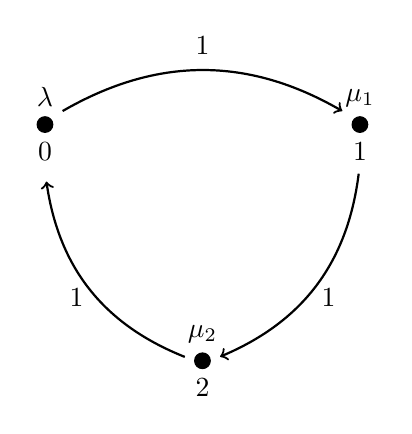
\begin{tikzpicture}
		\node[] (0) at (7,3.5) {};
		\node[draw=black, circle, inner sep=2pt, fill=black, label=below:{0}, label=above:{$ \lambda $}] (1) at (5,3) {};
		\node[] (A) at (5,2.4) {};
		\node[] (B) at (5.1, 3.1) {};
		
		\node[draw=black, circle, inner sep=2pt, fill=black, label=below:1, label=above:{$ \mu_1$}] (2) at (9,3) {};
		\node[] (C) at (8.9, 3.1) {};
		\node[] (D) at (9, 2.5) {};

		\node[draw=black, circle, inner sep=2pt, fill=black, label=below:2, label=above:{$ \mu_2 $}] (3) at (7,0) {};
		\node[] (E) at (7.1, 0) {};
		\node[] (F) at (6.9, 0) {};
		
		\node[] (X) at (5.4,0.8) {1};
		\node[] (Y) at (8.6,0.8) {1};
		\node[] (Z) at (7, 4) {1};
		
		\path []
		(B) edge[thick, bend left, ->] (C)
		(D) edge[thick, bend left, ->] (E)
		(F) edge[thick, bend left, ->] (A);
		
		
	\end{tikzpicture}
\end{multicols}

Quello che è interessante chiedersi è, se facciamo passare molto tempo, qual è la percentuale di tempo in cui nel negozio c'è un cliente e quella in cui non c'è nessun cliente (nel negozio può rimanere al massimo un cliente alla volta).

Torniamo ai processi di pura nascita. Sia $ S $ lo spazio degli stati:

$$ \forall s \in S, \quad v_s > 0 $$
$$ \forall s,s' \in S \quad s' \ne s \quad a_{s,s'} $$
$$ \sum_{\begin{array}{c}
	s' \in S \\ 
	s' \ne s
	\end{array}} a_{s,s'} = 1$$

Sia $\rho_s$ la distribuzione iniziale. Possiamo far vedere che un processo di tipo esponenziale corrisponde ad una catena di Markov omogenea continua. Il motivo di questa corrispondenza risiede nella proprietà dell'assenza di memoria della distribuzione esponenziale. \\
\\
Gli esempi visti fin'ora fanno parte di una classe di processi esponenziali detti \textbf{processi di nascita e morte} dove $ S = \mathbb{N} $ oppure $ S = [O, M] \in \mathbb{N} $. Per i processi di pura nascita, per ogni stato abbiamo due parametri: $\lambda_0, \forall s \ge 1 \lambda_s, \mu_s$

I processi di pura nascita sono un caso particolare dove $\mu_s = 0$.

Per ogni stato abbiamo due tempi esponenziali, uno di parametro $\lambda_s$ e uno di parametro $\mu_s$. Consideriamo il più piccolo tra $\lambda_{s}$ e $\mu_s$; se è $\lambda_{s}$, andremo nello stato $ s+1 $, altrimenti $ s-1 $. Nel caso dello stato 0 abbiamo solo $\lambda_0$, perché non ci sono stati con indice negativo. 

Se voglio descriverlo come processo esponenziale, avremo che $ v_0 = \lambda_0 $, $ s > 1 $ e $ v_s = \lambda_s + \mu_s $ perché se ci troviamo nello stato 0, il tempo che rimaniamo nello stato sarà $\lambda_0$; altrimenti, il tempo esponenziale che rimaniamo nello stato sarà il minimo tra $\lambda_s$ e $ \mu_s $. Ma noi abbiamo visto che se abbiamo due variabili con distribuzione esponenziale indipendente, il più piccolo dei due ha una distribuzione esponenziale che è pari alla somma dei parametri ($ \lambda_s +\mu _s $). 

Infine, la probabilità che tra i due il minimo sia $\lambda_s$ è dato da $\frac{\lambda_s}{\lambda_s + \mu_s}$; questo caso e il caso in cui $\mu_s$ sia il minimo tra i due sono riassunti nelle formule sottostanti:

$$ a_{s,s+1} = \frac{\lambda_s}{\lambda_s + \mu_s} \qquad a_{s,s-1} = \frac{\mu_s}{\lambda_s + \mu_s} \qquad a_{0,1} = 1$$

Anche nei processi di nascita e morte si può verificare esplosione. Se i $\lambda_s$ sono tutti maggiorati da una costante, non si può avere esplosione, e nemmeno se i $\lambda_i$ crescono come $ s $, ovvero $\lambda_s = s \cdot \lambda$ (quindi crescono linearmente con una qualche costante $ s $). %TODO cioè non ho capito se si può verificare epslosione o meno

Vediamo qual è l'attesa del tempo con cui possiamo andare da uno stato all'altro. Sia $ T_s $ il tempo per andare da $ s $ a $ s+1 $. 

Consideriamo l'attesa di $ T_s $, $ P(T_s) $:
$$ P(T_0) = \frac{1}{\lambda_0}$$
Consideriamo il caso generale $ s \ge 1 $; definiamo $ I_s $:
$$ I_s = \begin{cases}
	0, & \text{ se da } s \text{ passiamo a } s-1 \\
	1, & \text{ se da } s \text{ passiamo a } s+1 \\
\end{cases}$$
\begin{align*}
	P(T_s | I_s = 1) & = \frac{1}{\lambda_s + \mu_s} \\
	P(T_s | I_s = 0) & = \frac{1}{\lambda_s + \mu_s} + P(T_{s-1}) + P(T_s) 
\end{align*}

Se $ I_s = 1 $, allora passiamo allo stato $ s+1 $.

Se invece $ I_s = 0$, vuol dire che passiamo allo stato $ s-1 $; per tornare allo stato $ s+1 $, siccome possiamo fare solo salti di 1, dovremo prima tornare allo stato $ s $ e poi andare allo stato $ s+1 $.

Il tempo per andare dallo stato $ s $ allo stato $ s' $, con $ s' > s $:
$$ T_s + T_{s+1} + ... + T_{s'+1} $$
Quindi possiamo scrivere infine l'attesa di $ T_s $:
\begin{align*}
	P(T_s) & = P(T_s | I_s = 0)P(I_s = 0) + P(T_s | I_s = 1)P(I_s = 1) \\
	& = \frac{\lambda_s}{\lambda_s + \mu_s}\frac{1}{\lambda_s + \mu_s} + \frac{\mu_s}{\lambda_s + \mu_s} \left( - \frac{1}{\lambda_s + \mu_s} P(T_{s-1}) + P(T_s) \right) \\
	& = \frac{1}{\lambda_s + \mu_s} + \frac{\mu_s}{\lambda_s + \mu_s}\left(P(T_{s-1}) + P(T_s) \right) \\
	P(T_s)\left(1 - \frac{\lambda_s}{\lambda_s + \mu_s} \right) & = \frac{1}{\lambda_s + \mu_s} + \frac{\mu_s}{\lambda_s + \mu_s} P(T_{s-1}) \\
	P(T_s) & = \frac{1}{\lambda_s} + \frac{\mu_s}{\lambda_s} P(T_{s-1})
\end{align*}

Siccome $ P(T_0) = \frac{1}{\lambda_0}$, posso calcolare induttivamente (grazie alla formula sopra) tutte le attese di $ T_s $

\paragraph{Esempio} Vediamo un processo di nascita e morte con $\lambda_s = \lambda$ e $\mu_s = \mu$; questo corrisponde ad un processo di coda $ M/M/1 $, dove $\lambda$ è il parametro di Poisson degli arrivi e $ \mu $ è il parametro del tempo di servizio. Supponiamo $\mu \ne \lambda$:

$$ P(T_0)  = \frac{1}{\lambda} \qquad P(T_s) = \frac{1}{\lambda} + \frac{\mu}{\lambda} P(T_{s-1})$$

\begin{align*}
	P(T_1) & = \frac{1}{\lambda} + \frac{\mu}{\lambda} \frac{1}{\lambda} \\
	p(T_2) & = \frac{1}{\lambda} + \frac{\mu}{\lambda}\left( \frac{1}{\lambda} + \frac{\mu}{\lambda}\frac{1}{\lambda} \right)\\
	P(T_1) & = \frac{1}{\lambda} \left( 1 + \frac{\mu}{\lambda} \right) \\
	P(T_2) & = \frac{1}{\lambda} \left(1 + \frac{\mu}{\lambda} + \left(\frac{\mu}{\lambda}\right)^2 \right) \\
	... & \\
	P(T_s) & = \frac{1}{\lambda} \left( \frac{1 - \left(\ddfrac{\mu}{\lambda}\right)^{s+1}}{1 - \ddfrac{\mu}{\lambda}} \right) \\
	& = \frac{1 - \left(\ddfrac{\mu}{\lambda}\right)^{s+1}}{\lambda - \mu}
\end{align*}

Se $\lambda = \mu$:

$$ P(T_s) = \frac{1}{\lambda}(s+1) $$

Per andare da $ s $ a $ s' $, l'attesa sarà
$$ T_s + T_{s+1} + T_{s'-1} $$

%TODO 2020-11-25
L'esempio del lustrascarpe non è un processo di nascita e morte, perché ??? %TODO

Vediamo un processo di nascita e morte che modella la crescita (e decrescita) di una popolazione.

\subsection{Modello di crescita lineare con immigrazione}
In questo modello gli individui possono replicarsi: da un individuo se ne genera un altro, oppure morire. Il tempo dello sdoppiamento è un esponenziale di parametro $\lambda$, il tempo di morte è un esponenziale di parametro $\mu$. 

Ci interessa ??? %TODO

C'è però anche un afflusso di individui dall'esterno (dati dall'immigrazione); $\theta$ è il tempo associato con l'immigrazione. 

Sia lo spazio degli stati $ S = \mathbb{N} $. 

Sia $\mu_n = m\cdot \mu$ %TODO è m\cdot\mu oppure n\cdot\mu?
 e $\lambda_n = n\cdot \lambda + \theta$.
 
 Se abbiamo $ n $ individui, a ogni individuo sarà associato un tempo esponenziale (il tempo della morte). Quando un individuo muore, la popolazione diminuirà di 1 al minimo dei tempi associato agli individui. Il minimo tra $ n $ variabili aleatorie con distribuzione esponenziale è pari a ?? %TODO
 
 Quindi ? %TODO
 parametro del minimo è $ n\mu $. Analogo per $\lambda n$: ... %TODO
 
 Definiamo $ X_t $ la variabile aleatoria che descrive il numero totale degli individui. Sia $ M(t) $ l'attesa di $ X_t $: $ M(t) = P(X_t) $.
 
 Fissato un certo $ i \in \mathbb{N} $, la distribuzione iniziale sarà $ \rho_i = 1, \rho_s = 0 s\ne i $: all'inizio la popolazione comprende $ i $ individui. 
 
 Per calcolare $ M(t) $ usiamo un'equazione differenziale:
 
	$$ M(t+h) = P(X_{t+h}) = P(P(X_{t+h} | X_t))$$
	$$ X_{t+h} = \begin{cases}
		X_t + 1, & \text{con probabilità } (\theta + \lambda X_t)h + o(h) \\
		X_t-1, & \text{con probabilità } (\mu X_t)h + o(h) \\
		X_t, & \text{con probabilità } 1 - (\theta + X_t(\lambda + \mu)) + o(h)
	\end{cases} $$ %TODO quando aumentiamo di 1???
	
La probabilità di passare in uno stato più di 1 è un infinitesimo di ordine superiore ??? %TODO

\begin{align*}
	M(t+h) - M(t) & = P(P(X_{t+h} | X_t )) - M(t) \\
	& = \bar{P(X_t)} + (\theta + (\lambda - \mu)) P(X_t)) + o(h) - \bar{P(X_t)} \\ %TODO parentesi non bilanciate
	& = \theta + (\lambda - \mu)) M(t) + \frac{o(h)}{h} %TODO parentesi non bilanciate
\end{align*}

Facendo tendere $ h $ a 0 calcoliamo la derivata:
$$ M(t) = (\lambda - \mu) M(t) + \theta $$

La condizione iniziale è $ M(0) = i $; per risolvere l'equazione differenziale introduciamo una funzione $ h $:

\begin{align*}
	h(t) & = (\lambda - \mu)M(t) + \theta \\
	h'(t) & = (\lambda - \mu)M'(t) \\
	& = (\lambda - \mu)^2 M(t) + (\lambda - \mu)\theta \\
	& = (\lambda - \mu)((\lambda - \mu)M(t) + \theta) \\
	& = (\lambda - \mu)h(t) \\
	\frac{h'(t)}{h(t)} & = \lambda - \mu \\
	\Rightarrow \frac{\partial \log(h(t))}{\partial t} & = \lambda - \mu
\end{align*}

Supponiamo $ \lambda \ne \mu $:
$$ \log(h(t)) = (\lambda - \mu)t + c $$
Sia $ e^c = k $:
\begin{align*}
	 h(t) & = K e^{(\lambda - \mu)t} \\
	 \Rightarrow (\lambda - \mu)M(t) + \theta & = Ke^{(\lambda - \mu)t}
\end{align*}
Mi rimane da calcolare $ K $; sapendo che $ M(0) = i$:
\begin{align*}
	(\lambda - \mu)i + \theta & = k \\
	\Rightarrow M(t) & = \frac{(\lambda - \mu)i + \theta}{\lambda - \mu} \cdot e^{(\lambda - \mu)t} - \frac{\theta}{\lambda - \mu}
\end{align*}

Se $ \lambda = \mu $:
$$ h'(t) = (\lambda - \mu)h(t) = 0 $$

Se la derivata di $ h $ è 0, allora $ h $ sarà pari a una costante:

\begin{align*}
	h(t) & = ct + d \\
	\Rightarrow M(t) & = \theta t + i
\end{align*}

Nel caso $\mu = \lambda$ quindi la popolazione cresce linearmente con l'immigrazione, nell'altro caso cresce se $ \lambda > \mu $ la crescita è esponenziale, altrimenti si stabilizza e cresce grazie all'immigrazione. Può avvenire l'esplosione? No, perché in questo caso le costanti crescono ??? %TODO

Abbiamo calcolato solo l'attesa del numero di individui; possiamo calcolare però le probabilità di transizione, tornando ai modelli di pura nascita.

\subsection{Modello di pura nascita}
$ S = \mathbb{N} ??? \mu_0 = \mu_1 = ... = \mu_n = 0 $ %TODO

Sia $ s \in \mathbb{N} $; sia $ T_s $ il tempo di permanenza nello stato $ s $. $ T_0, T_1, ... $ sono esponenziali di parametro $\lambda_s$ e sono indipendenti. 

Vogliamo calcolare $ P_{i,j}(T): $

$$ P_{i,j}(T) = (X_t = j | X_0 = i) \qquad \qquad j \ge i $$

Nel caso dei processi di pura nascita lo stato può solo crescere, quindi la probabilità di andare da $ j $ a $ i $ con $ i < j $ è 0. 

$$ P_{i,j}(t) = P(T_i > t) = e^{-\lambda_i t} $$

Se $ i < j $: 
\begin{align*}
	P_{i,j}(t) & = P(T_i + Y_{i+1} + ... + T_j > t_1, T_i + ... + T_{j-1} \le t) \\
	& = P((T_i + T_{i+1} + ... + T_j > t) - (T_i + T_{i+1} + ... + T_{j-1} > t))
\end{align*}

Il secondo evento è più piccolo del primo, è contenuto nel primo

$$ = P(T_i + T_{i+1} + ... + T_j > t) - P(T_i + T_{i+1} + ... + T_{j-1} > t) $$

Supponiamo $\lambda_s \ne \lambda_{s'}$, per $ s \ne s' $

$$ = \sum_{k=1}^{j} e^{-\lambda_k t} \prod_{\begin{array}{c}
	r \ne k \\ %TODO controlla sia \ne
	r = i
	\end{array}}^{j} \frac{\lambda_r}{\lambda_r - \lambda_k} - \sum_{k=1}^{j-1} e^{-\lambda_k t} \prod_{\begin{array}{c}
	r \ne k \\ %TODO controlla sia \ne
	r = i
	\end{array}}^{j-1} \frac{\lambda_r}{\lambda_r - \lambda_k}$$

In questo caso c'è la possibilità che ci sia esplosione:
$$ \sum_j P_{i,j}(t) < 1 \qquad \qquad ???$$ %TODO

\paragraph{Processo di Yule} Un caso particolare è il processo di Yule, in cui $\lambda_j = j\lambda$ con $\lambda > 0$.

Lo spazio degli stati non parte da 0: $ S = \{1,2,3...\} $

In questo caso non c'è esplosione: se i $\lambda_j$ crescono linearmente,

$$ \sum_j^{\infty} \frac{1}{\lambda_j} = 1 \qquad \qquad ??? = +\infty$$ %TODO

\section{Equazioni di Kolmogorov}

Vediamo ora come si può impostare in generale il calcolo della probabilità di transizione per le catene di Markov con tempo continuo. ?? %TODO
 Si può dimostrare che deve soddisfare le equazioni in avanti di Kolmogorov e le equazioni all'indietro di Kolmogorov. 

Partiamo da un processo di tipo esponenziale:

?? %TODO

$ q:{s,s'} $ è detta intensità della transizione da $ s $ a $ s' $.

$$ P_{s,s'}(h) = q_{s,s'}h + o(h) $$

$ 1 - e^{-v_s h} $ è la probabilità che il tempo esponenziale sia minore di $ h $. 

Quando scade questo tempo ??? %TODO

Quindi 

\begin{align*}
	(1 - e^{-v_s h})a_{s,s'} + o(h) & = (v_s h + c(h)) a_{s,s'} + o(h) \\ %TODO controlla parentesi
	& = v_s a_{s,s'} h + o(h) & = q_{s,s'} h + o(h)
\end{align*}

Vogliamo ottenere delle equazioni che sono soddisfatte dalle probabilità di transizione.

\subsection{Equazioni all'indietro di Kolmogorov (Kolmogorov backward equation)}

Consideriamo un intervallo $ [0, t+h] = [0, h] \cup [h, t+h] $. %TODO controlla sia o oppure 0

Consideriamo la probabilità

$$ P_{s,s'} (t+h) = \sum_{s''} P_{s,s''}(h)P{s'', s'}(t) $$

Possiamo approssimare questa probabilità:

\begin{align*}
	& = \sum_{s'' \ne s} (q_{s,s''}h + o(h))P_{s'',s'}(t) + P_{s,s}(h) \\
	& = \sum_{s'' \ne s} ... + \underbrace{e^{-v_s h} + o(h)}_{1 - v_s h + o(h)}\\ %TODO
	& = \sum_{s'' \ne s} ... + (1 - v_s h + o(h))P_{s,s'}(t) %TODO
\end{align*}

Voglio scrivere un'equazione differenziale ??? %TODO

Considero 

$$ \frac{P_{s,s'}(t+h) - P_{s,s'}(t)}{h} = \frac{-v_s h + o(h)}{h} P_{s,s'}(t) + \frac{\sum_{s'' \ne s} (q_{s,s''} h + o(h)) }{h} P_{s'',s'}(t) $$

Per calcolare la derivata, facciamo tendere $ h $ a 0:

\begin{align*}
	\underset{h \to 0}{\longrightarrow} \qquad & -v_s P_{s,s'}(t) + \sum_{s' \ne s}(t) + \sum_{s' \ne s} q_{s,s''} - P_{s'',s'}(t) \\
	\frac{\partial}{\partial t} P_{s,s'}(t) = & -v_s P_{s,s'}(t) + \sum_{s'' \ne s} q_{s,s''} P_{s'',s'}(t) 
\end{align*}

$ \frac{\partial}{\partial t} P_{s,s'}(t) $ è l'equazione di Kolmogorov all'indietro. Queste equazioni collegano tra loro le probabilità di transizione con lo stesso punto di arrivo. 

\paragraph{Esempio} $ S = \{0,1\} $; abbiamo $ v_0, v_1 $
$$ \begin{array}{cc}
 	q_{0,1} = v_0 & q_{1,0} = v_1 \\
 	a_{0,1} = 1 & a_{1,0} = 1
\end{array} $$

\begin{align*}
	\frac{\partial}{\partial t} P_{0,1}(t) & = -v_0 P_{0,1}(t) + v_0 P_{1,0}(t) \\
	\frac{\partial}{\partial t} P_{0,0}(t) & = -v_0 P_{0,0}(t) + v_0 P_{1,0}(t) 
\end{align*} 

%TODO 2020-12-1
Un modo per vedere le equazioni all'indietro è rappresentando la catena di Markov con un grafico:
\begin{center}
	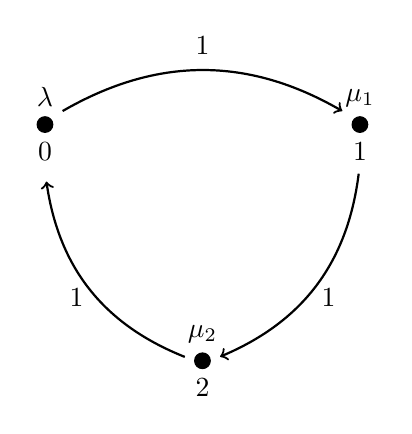
\begin{tikzpicture} %TODO rincontrolla grafico
		\node[] (0) at (7,3.5) {};
		\node[draw=black, circle, inner sep=2pt, fill=black, label=below:{0}, label=above:{$ \lambda $}] (1) at (5,3) {};
		\node[] (A) at (5,2.4) {};
		\node[] (B) at (5.1, 3.1) {};
		
		\node[draw=black, circle, inner sep=2pt, fill=black, label=below:1, label=above:{$ \mu_1$}] (2) at (9,3) {};
		\node[] (C) at (8.9, 3.1) {};
		\node[] (D) at (9, 2.5) {};
		
		\node[draw=black, circle, inner sep=2pt, fill=black, label=below:2, label=above:{$ \mu_2 $}] (3) at (7,0) {};
		\node[] (E) at (7.1, 0) {};
		\node[] (F) at (6.9, 0) {};
		
		\node[] (X) at (5.4,0.8) {1};
		\node[] (Y) at (8.6,0.8) {1};
		\node[] (Z) at (7, 4) {1};
		
		\path []
		(B) edge[thick, bend left, ->] (C)
		(D) edge[thick, bend left, ->] (E)
		(F) edge[thick, bend left, ->] (A);
	\end{tikzpicture}
\end{center}

Ad ogni stato è associato $ v_1 $ ??? %TODO

Le frecce sono ??? %TODO

Ad ogni freccia possiamo associare l'intensità $ q_{i,j} $

Le equazioni all'indietro si ottengono così:

$$ P_{s,s'}'(t) = -v_sP_{s,s'} + \sum_{s''\ne s} q_{s,s''} P_{s'',s}(t)$$

Guardiamo il grafico ??? %TODO

Vediamo l'esempio più semplice, quello in cui $ S = \{0,1\} $; sia $ s' = 0 $. Abbiamo $ v_0 = \lambda, v_1 = \mu $. Abbiamo anche che $ q_{0,1} = \lambda, q_{1,0} = \mu $.

Le equazioni all'indietro sono:
\begin{align*}
	P_{0,0}'(t) & = \lambda[P_{1,0}(t) - P_{0,0}(t)] \\
	P_{1,0}'(t) & = \mu [P_{0,0}(t) - P_{1,0}(t) ] \\
	\frac{d}{dt} [\mu P_{0,0}(t) + \mu P_{0,0}'(t) + \lambda P_{1,0}'(t) ] & = 0 \\
	\lambda P_{1,0}(t)] & = \mu P_{0,0}(t) + \lambda P_{1,0}(t) = c \\ %TODO ricontrolla
	\mu P_{0,0}(0) + \lambda P_{1,0}(0) & = c \\
	\mu \cdot 1 + \lambda \cdot 0 & = c \\
	\Rightarrow c & = \mu
\end{align*}

$ \mu P_{0,0}(t) + \lambda P_{1,0}(t) $ è uguale ad una costante $ c $ perché non cambia nel tempo; quanto vale $ c $? Per scoprirlo abbiamo posto $ t = 0 $.

Quindi abbiamo che 

\begin{align*}
	\lambda P_{0,0}(t) + \mu P_{0,0}(t) & = \mu \\
	\lambda P_{1,0}(t) & = \mu(1 - P_{0,0}(t)) \\
	P_{0,0}'(t)\mu & = [1 - P_{0,0}(t)] - \lambda P_{0,0}(t) \\
	& = \mu - (\mu + \lambda) P_{0,0}(t)
\end{align*}

Definiamo 

$$ h(t) = P_{0,0}(t) - \frac{\mu}{\mu + \lambda}$$

\begin{align*}
	h'(t) & = \mu - (\mu - \lambda)(h(t) + \frac{\mu}{\mu + \lambda}) \\
	& = -(\mu + \lambda)h(t) \\
	\frac{h'(t)}{h(t)} & = -(\mu + \lambda) \\
	& = \frac{\partial}{\partial t} \log(h(t)) \\
	\log h(t) & = -(\mu + \lambda)t + c \\
	h(t) & = K e^{-(\mu + \lambda)t}
\end{align*}

Quando vale $ K $?

\begin{align*}
	h(t) & = P_{0,0}(t) - \frac{\mu}{\mu + \lambda} \\
	h(0) & = P_{0,0}(0) - \frac{\mu}{\lambda + \mu} \\
	& = \ - \frac{\mu}{\mu + \lambda} \\
	& = \frac{\lambda}{\lambda + \mu} \\
	h(t) & = \frac{\lambda}{\mu + \lambda}e^{(-\mu + \lambda)t} \\
	P_{0,0}(t) & = \frac{\lambda}{\mu + \lambda}e^{-(\mu + \lambda)t} + \frac{\mu}{\mu + \lambda} \\
	\lambda P_{0,0}(t) & = \mu - (\mu + \lambda) P_{0,0}(t) \\
	P_{1,0} (t) & = \frac{\mu}{\lambda} - \frac{(\mu + \lambda)}{\lambda} \left(\frac{\lambda}{\mu + \lambda} e^{-(\mu + \lambda)t} + \frac{\mu}{\mu + \lambda}\right) \\
	& = \frac{\mu}{\mu + \lambda}e^{-(\mu + \lambda)t} + \frac{\mu}{\mu + \lambda}
\end{align*}

Facciamo tendere $ t $ all'infinito:

$$ P_{0,0}(t) \to \frac{\mu}{\mu + \lambda} \quad \text{ e } \quad P_{1,0}(t) \to \frac{\mu}{\mu + \lambda}$$

Quindi se facciamo passare molto tempo le probabilità di andare nello stato 0 sia partendo da 0, sia partendo da 1, tendono allo stesso limite. 

Per quel che riguarda $ P_{0,1}(t) $ e $ P_{1,1}(t) $ non occorre rifare i calcoli, perché è come se si scambiassero di nome gli stati e quindi basta scambiare $\mu$ e $\lambda$:

\begin{align*}
	P_{1,1}(t) & = \frac{\mu}{\mu + \lambda} e^{-(\mu + \lambda)t} + \frac{\lambda}{\lambda + \mu} \\
	P_{0,1}(t) & = \frac{\lambda}{\mu + \lambda} e^{-(\mu + \lambda)t} + \frac{\lambda}{\lambda + \mu}
\end{align*}

Se $ t \to \infty $:

$$ P_{0,1}(t) \to \frac{\lambda}{\mu + \lambda} \quad \text{ e } \quad P_{1,1}(t) \to \frac{\lambda}{\mu + \lambda}$$

Si può vedere che questo valore è anche la percentuale di tempo che la catena di Markov si trova nello stato 1. %TODO riascolta

\subsection{Equazioni in avanti di Kolmogorov (Kolmogorov forward equations )}
Consideriamo un intervallo di tempo $ (0, t+h] $. 

Nelle equazioni all'indietro di Kolmogorov abbiamo diviso l'intervallo da 0 a $ h $; qui dividiamo in due intervalli $ (0, t] $ e $ (t, t+h] $. 

\begin{align*}
	P_{s,s'}(t+h) & = P_{s,s'}(t) P_{s',s'}(h) + \sum_{s'' \ne s} P_{s,s''}(t)P_{s'',s'}(h) \\ %TODO rincontrolla
	P_{s',s'}(h) & = 1 - v_{s'} h + o(h) \\
	P_{s'',s'}(h) & = q_{s'',s'}h + o(h) \\
	\frac{P_{s,s'}(t+h) - P_{s,s'}(t)}{h} & = \frac{(-v_{s'} h + o(h))}{h}P_{s,s'}(t) + \frac{\sum_{s'' \ne s'}(q_{s'',s'} h + o(h) ) }{h} P_{s,s''}(t)
\end{align*}

È legittimo passare al limite? Nei casi che vedremo questo passaggio è sempre legittimo; facciamo tendere $ h $ a 0: %TODO riascolta

$$ P_{s,s'}'(t) = -v_{s'} P_{s,s'}(t) + \sum_{s'' \ne s' } q_{s'',s'}P_{s,s''}(t) $$

Anche di questa equazione si può dare un'interpretazione grafica. 

A differenza delle equazioni all'indietro, questa collega tra loro ??? %TODO
teniamo fisso il punto di partenza. Sulle altre invece tenevamo fermo il punto di d'arrivo. 

\begin{align*}
	P_s(t) & = P(X_t = s) \\
	& = \sum \rho_{s'} P_{s',s}(t) \\
	\frac{\partial}{\partial t}P_s(t) & = \sum_{s'} \rho_{s'} \frac{\partial}{\partial t} P_{s',s}(t) \\
	P_s'(t) & = -v_s P_s(t) + \sum_{s'}P_{s'}(t) q_{s',s}
\end{align*}

\paragraph{Esempio }Vediamo ora il caso più semplice in cui $ S = \{0,1\} $:
$$ \begin{array}{c}
	v_0 = \lambda = q_{0,1} \\
	v_1 = \mu = q_{1,0}
\end{array} $$

\begin{align*}
	P_{0,0}'(t) & = -\lambda P_{0,0}(t) + \mu P_{0,1}(t) \\
	P_{0,1}'(t) & = -\mu P_{0,1}(t) + \lambda P_{0,1}(t)
\end{align*}

\begin{align*}
	P_{0,0}(t) + P_{0,1}(t) & = 1 \\
	P_{0,1}(t) & = 1 - P_{0,0}(t) \\
	P_{0,0}'(t) & = - \lambda P_{0,0}(t) + \mu(1 - P_{0,0}(t)) \\
	P_{0,0}'(t) & = -(\lambda + \mu)P_{0,0}(t) + \mu
\end{align*}

Definiamo 

$$ h(t) = P_{0,0}(t) + \frac{\mu}{\lambda + \mu} $$

\begin{align*}
	h'(t) & = -(\lambda + \mu)(h(t) + \frac{\mu}{\lambda + \mu}) + \mu \\
	& = -(\lambda + \mu) h(t) \\
	h(t) & = Ke^{-(\lambda + \mu)t} \\
	h(t) & = \frac{\mu}{\lambda + \mu} + \frac{\lambda}{\lambda + \mu}e^{-(\lambda + \mu)t} \\
	P_{1,1}(t) & = 1 - P_{0,0}(t) \\
	& = \frac{\lambda}{\lambda + \mu} - \frac{\lambda}{\lambda + \mu} e^{-(\lambda + \mu)t} \\
	P_{1,1}(t) & = \frac{\lambda}{\lambda + \mu} + \frac{\mu}{\lambda + \mu}e^{-(\lambda + \mu)t} \\
	P_{1,0}(t) & = \frac{\mu}{\lambda + \mu} - \frac{\mu}{\lambda + \mu}e^{-(\lambda + \mu)t} \\
	P_{0,0}(t) + P_{0,1}(t) & = 1 \\
	P_{1,0}(t) + P_{1,1}(t) & = 1
\end{align*}

\subsubsection{Esempio - Processi di pura nascita}

$$ S = \mathbb{N} \qquad \qquad \begin{array}{cc}
	v_s = \lambda_s & a_{s,s+1} = 1 \\
	q_{s,s+1} = \lambda_s
\end{array}$$

Fissiamo $ \bar{s} $ stato di partenza; quali sono le equazioni in avanti?

\begin{align*}
	P_{\bar{s},s}'(t) & = -\lambda_s P_{\bar{s},s}(t) + \lambda_{s-1P_{\bar{s},s-1}(t)} \\
	P_{\bar{s},\bar{s}}'(t) & = -\lambda_{\bar{s}} P_{\bar{s},\bar{s}}(t) \\ %TODO riascolta perché non possiamo riscrivere \bar{s} - 1
	P_{\bar{s},\bar{s}}(t) & = Ke^{-\lambda_{\bar{s}}t} \\
	& = e^{-\lambda_{\bar{s}} t}
\end{align*}

$ K $ deve essere uguale a 1 perché ??? %TODO

$$ P_s(t) = P_{\bar{s},s}(t) $$

Supponiamo $ s > \bar{s} $; allora:

\begin{align*}
	P_s'(t) & = -\lambda_s P_s(t) + \lambda_{s-1}P_{s'-1}(t) \\ %TODO controlla non ci sia un \rho
	P_s'(t) + \lambda_s P_s(t) & = \lambda_{s-1} P_{s-1}(t) \\
\end{align*}

Osserviamo che 
\begin{align*}
	\frac{\partial}{\partial t}(e^{-\lambda_s t} P_s(t)) & = \lambda_s e^{\lambda_s t} P_s(t) + e^{\lambda_s t}P_s'(t) \\
	e^{-\lambda_s(t)} \frac{\partial}{\partial t}(\partial t)(e^{\lambda_s t}P_s(t)) & = \lambda_{s-1} P_{s-1}(t) \\
	\frac{\partial}{\partial t}(e^{\lambda_s t} P_s(t)) & = \lambda_{s-1}e^{\lambda_s t} P_{s-1}(t) \\
	e^{\lambda_s t}P_s(t) & = P_s(0) + \int_{0}^{t} \lambda_{s-1}e^{\lambda_s u} P_{s-1}(u) du \\
	P_s(t) & = P_s(0) e^{\lambda t} + e^{-\lambda t} \int_0^t \lambda_{s-1} e^{\lambda_s u} P_{s-1}(u)du \\
	P_s(t) & = P_{\bar{s}, \bar{s}}(t) \\
	& = e^{-\lambda_{\bar{s}} t}
\end{align*}

Possiamo ottenere tutti i valori delle probabilità di transizione. 

Un caso particolare è il processo di Yule, in questo caso $ S = \mathbb{N} \setminus \{0\} $: è sempre un processo di pura nascita ma non consideriamo lo stato 0; parte infatti da 1, con $\lambda_s = s\cdot \lambda$. Se lo pensiamo come un processo di una popolazione, ad ogni individuo è associato un tempo esponenziale di parametro $\lambda$ e, allo scadere del tempo, l'individuo si sdoppia. Allo stato $ k $ ci sono $ k $ individui. Se consideriamo un intervallo $ h $ ??? %TODO
dobbiamo fare il minimo tra due variabili \texttt{etc. riascolta} %TODO

Si può dimostrare che 
$$ p_{1,s}(t) = e^{-\lambda t}(1 - e^{-\lambda t})^{s-1} $$

La dimostrazione può avvenire in vari modi. ?? %TODO

Equazioni di Kolmogorov in avanti:

\begin{align*}
	P_{1,1}(0) & = 1 \\
	P_{1,s}'(t) & \overset{?}{=} -s \lambda P_{1,s}(t) + (s-1)\lambda P_{1,s-1}(t)
\end{align*}

Non sappiamo se l'uguaglianza vale, dobbiamo verificare che soddisfi le equazioni in avanti di Kolmogorov. 

%2020-12-2

Quindi calcoliamo la derivata:

\begin{align*}
	P_{1,s}'(t) & = \lambda e^{-\lambda t }(1 - e^{-\lambda t})^{s-1} + \lambda e^{-\lambda t} e^{-\lambda t}(s-1)(1-e^{-\lambda t})^{s-2}  + \lambda e^{-\lambda t(1 - (1- e^{-\lambda t}))} \\ %TODO ricontrolla
	& = -\lambda s e^{-\lambda t}(1 - e^{-\lambda t})^{s-1} + ??? \lambda t(1 -\lambda t)^{s-2} %TODO
\end{align*}

Questa è la soluzione partendo da 1; qual è la soluzione partendo da un altro stato? In generale:

\begin{align*}
	P_{s,s'} & = \binom{s'-1}{s-1}e^{-s\lambda t} (1 - e^{-\lambda t})^{s'-s} \\
	P_{1,s'}(t) & = e^{-\lambda t} (1 - e^{-\lambda t})^{s'-1}
\end{align*}

L'ultima equazione è la distribuzione geometrica; la distribuzione geometrica infatti è del tipo $ (1-p)^{k-1} $, con $ p,k = 1, 2, ... $. È collegata con lo schema di Bernoulli. Quindi quella soprastante è una distribuzione geometrica con $ p = e^{-\lambda t} $.

Facciamo ora un'\textbf{osservazione}, collegata all'interpretazione del processo di Yule come processo di popolazione: $ P_{s,s'}(t) $ vuol dire che la popolazione all'inizio ha $ s $ individui, e ci stiamo chiedendo qual è la probabilità che al tempo $ t $ abbia $ s' $ individui. $ P_{s,s'}(t) $ si può vedere come la somma del numero di individui che discende dagli $ s $ iniziali, ovvero la somma di $ s $ variabili aleatorie indipendenti con distribuzione geometrica di parametro $ e^{-\lambda t} $.

La distribuzione geometrica è la distribuzione nel tempo del primo successo; se invece anziché la prima vediamo la $ s $-esima volta, questo tempo lo possiamo suddividere come la somma di $ s $ variabili aleatorie indipendenti: bisogna vedere qual è il tempo in cui dobbiamo aspettare per la prima volta ??? %TODO

Qual è la probabilità che fino al tempo $ s-1 $ abbiamo avuto $ s-1 $ successi? È la distribuzione binomiale:

$$ \binom{s'-1}{s-1}e^{-(s-1)\lambda t}(1-e^{-\lambda t})^{s'-s}e^{-\lambda t} = \binom{s'-1}{s-1} e^{-s\lambda t}(1-e^{-\lambda t})$$

Questo verifica le equazioni di Kolmogorov in avanti. 

%TODO mia domanda

Vediamo ora quando convergono ??? %TODO

Supponiamo che da $ P_{s,s'}(t) $ converga per $ t \to \infty $ per tutti gli $ s $; Come ottengo il limite? %TODO in che senso

$$ \lim\lim\limits_{t \to \infty} P_{s,s'}(t) = P_{s'} $$ %TODO il secondo è P o p?

Scriviamo le equazioni in avanti:

$$ P_{s,s'}'(t) = -v_{s'} P_{s,s'}(t) + \sum_{s'' \ne s'}q_{s'',s} P_{s.s''}(t) $$

Supponiamo che le probabilità convergano. Allora 

$$ \underset{t \to \infty}{\longrightarrow} -v_{s'}p_{s'} + \sum_{s'' \ne s} q_{s'',s'}p_{s''} $$

Affinché converga, questa quantità deve essere uguale a 0. Infatti, supponiamo per assurdo che sia un valore diverso da 0. Allora potrebbe tendere a un valore ??? %TODO

??? sistema equazioni lineari ??? %TODO

?? caso più semplice %TODO

Sia $ S = \{0,1\} $, $ \bar{s} $ lo stato di partenza; le equazioni in avanti sono:

\begin{align*}
	P_{\bar{s},0}'(t) & = -\lambda P_{\bar{s},0}(t) + \mu P_{\bar{s},1}(t) \\
	P_{\bar{s},1}'(t) & = -\mu P_{\bar{s},1}(t) + \lambda P_{\bar{s},0}(t)) %TODO parentesi non bilanciate
\end{align*}

Siamo interessati solo al limite a cui tendono: %TODO ?? sicuri?

$$
\begin{cases}
	0 = -\lambda p_0 + \mu p_1 \\
	0 = -\mu p_1 + \lambda p_0 \\
	p_0 + p_1 = 1
\end{cases}
$$

\begin{multicols}{2}
	\begin{align*}
	p_1 & = 1-p_0 \\
	0 & = \lambda p_1 + \mu(1 - p_0) \\
	p_0 & = \frac{\mu}{\lambda + \mu} & p_1 = \frac{\lambda}{\lambda + \mu}
	\end{align*}
	\\
	\\
	\\
	?? %TODO
	\\
	distribuzione stazionaria
	\\
	??
\end{multicols}

Vediamo ora un esempio di distribuzione stazionaria e proviamo a calcolarla ?? %TODO

La distribuzione stazionaria è come un punto di equilibrio ?? %TODO 

Nei processi di nascita e morte non è detto ?? %TODO

Nei processi di pura nascita non c'è ?? %TODO

\paragraph{Esempio - Negozio di pulitura di scarpe} Sia $ S = \{0,1,2\} $

$$ \begin{array}{cccc}
	v_0 = \lambda & v_1 = \mu_1 & v_2 = \mu_2 & ?? \\
	a_{0,1} = 1 & a_{1,2} = 1 & a_{2,0} = 1 \\
	q_{2,0} = \mu_2 & q_{0,1} = \lambda & q_{1,2} = \mu_1
\end{array} $$

\begin{align*}
	\bar{P}_{\bar{s},0}(t) & = -\lambda P_{\bar{s}, 0}(t) + \mu_2 P_{\bar{s},2}(t) \\
	{P}_{\bar{s},1}'(t) & = -\mu_1 P_{\bar{s}, 1}(t) + \lambda P_{\bar{s},0}(t) \\
	{P}_{\bar{s},2}'(t) & = -\mu_2 P_{\bar{s}, 2}(t) + \mu_1 P_{\bar{s},1}(t)
\end{align*}

$$ 
	\begin{cases}
		-\lambda p_0 + \mu_2 p_2 = 0 \\
		-\mu_1 p_1 + \lambda p_0 = 0 \\
		-\mu_2 p_2 + \mu_1 p_1 = 1 \\
		p_0 + p_1 + p_2 = 1
	\end{cases}
$$

Abbiamo 4 equazioni e 3 incognite ??? %TODO

\paragraph{Esempio}

Abbiamo $ M $ macchine e 1 riparatore. Quando una macchina si guasta, viene messa in riparazione. Se c'è già una macchina in riparazione, si forma una coda. 

Prendiamo come stato il numero delle macchine in funzione; ??? %TODO

Il tempo di riparazione è un esponenziale di parametro $\mu$. Lo spazio degli stati è $ \{0, ..., M\} $. Supponiamo ci siano $ s $ macchine in funzione; le macchine in riparazione saranno $ M - s $. 

Il tempo della riparazione è $ v_s $. 

$$ \begin{array}{cc}
	v_s = s\lambda + \mu \; , & s \le M-1 \\
	s_M = M \lambda \; , & s = M
\end{array} $$

Quando scade $ v_s $, qual è la probabilità di andare nello stato $ s+1 $ e qual è la probabilità di andare nello stato $ s-1 $?

Sia $ s \le M-1 $:

\begin{align*}
	a_{s,s+1} & = \frac{\mu}{s\lambda + \mu} \\
	a_{s,s-1} & = \frac{s\lambda}{s\lambda + \mu} \\
	a_{M, M-1} & = 1 \\
	q_{s,s+1} & = \mu \\
	q_{s,s-1} & = s\lambda
\end{align*}

Sia $ s = M $:
\begin{align*}
	q_{M, M-1} & = M\lambda 
\end{align*}

$$ 	p_0, p_1, ..., p_m  $$ %TODO ???
$ 	s \le M-1 $:
\begin{align*}
	-p_s(\mu  +s\lambda) & = \mu p_{s-1} + (s+1)\lambda p_{s+1} 
\end{align*}
$ 	s = M $:
\begin{align*}
	-p_M M \lambda & = p_{M-1} \mu 
\end{align*}

$ 	p_0 + p_1 + ... + p_M < 1 $

\paragraph{Esempio}
Abbiamo visto esempi con un numero finito di stati; vediamo un esempio con un numero infinito di stati. Supponiamo di avere una coda $ M/M/1 $ (processo di nascita e coda ??? %TODO
dove gli arrivi sono un processo di Poisson di parametro $\lambda$, il tempo di servizio è un processo di Poisson di parametro $\mu$ e infine c'è un solo sportello. 

Prendiamo come stato il numero totale dei clienti nel sistema; quindi $ S = \mathbb{N} $. 

Prendiamo come distribuzione iniziale
$$ \rho_0 = 1$$
ovvero all'inizio non c'è nessun cliente. 

Mentre siamo nello stato $ 0 $, quando avviene il cambiamento di stato? È possibile solo se arriva un nuovo cliente; i clienti arrivano con processo di Poisson di parametro $\lambda$:
$$ v_0 = \lambda $$
$$ a_{0,1} = 1 $$

Se invece $ s \ge 1 $, un cambiamento di stato può avvenire in due modi: arriva un nuovo cliente oppure finiamo di servire un cliente. È il minimo tra due variabili esponenziali di parametri $\lambda$ e $\mu$:

\begin{align*}
	v_s & = \lambda + \mu \\
	a_{s,s+1} & = \frac{\lambda}{\lambda + \mu} & \text{il minimo corrisponde a } \lambda \\
	a_{s, s-1} & = \frac{\mu}{\lambda + \mu} & \text{il minimo corrisponde a } \mu \\
	q_{0,1} & = \lambda \\ 
	q_{s,s+1} & = \lambda \\
	 q_{s,s-1} & = \mu
\end{align*}
%TODO c'è qualcosa tipo vs * a_{s,s+1} in piccolo

Vogliamo vedere se c'è una distribuzione stazionaria e calcolarla. 

\begin{center}
	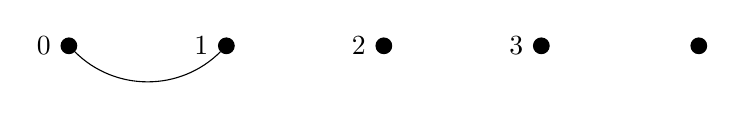
\begin{tikzpicture}
		\node[draw, circle, inner sep=2pt, fill=black, label=left:0] (0) at(-4, 0) {};
		\node[draw, circle, inner sep=2pt, fill=black, label=left:1] (1) at(-2, 0) {};
		\node[draw, circle, inner sep=2pt, fill=black, label=left:2] (2) at(0, 0) {};
		\node[draw, circle, inner sep=2pt, fill=black, label=left:3] (3) at(2, 0) {};	
		\node[draw, circle, inner sep=2pt, fill=black] (4) at(4, 0) {};	
		
		\draw[black] (0) to[out=-45,in=-135] (1) ;
	\end{tikzpicture}
\end{center}











\backmatter
% bibliography, glossary and index would go here.



\end{document}